\documentclass[UTF8]{ctexart}
\usepackage{amsmath, fancyhdr,geometry,tikz,pgfplots,tkz-euclide,setspace,graphicx}
\pagestyle{fancy}
\rhead{Academic Party 2.0 beta}
\geometry{left = 3.18cm, right = 3.18cm, top = 2.54cm, bottom = 2.54cm}
\renewcommand{\headrulewidth}{0.1pt}
\renewcommand{\footrulewidth}{0.1pt}
\title{Calculus BC}
\author{Academic Party 2.0 beta}
\begin{document}
\maketitle
\tableofcontents
\section{Limits}
\subsection{Limit at a Point}
\subsubsection{Definition of Limits}
\paragraph{探索}
如果你面前摆着一盘比萨,你会非常愿意把头伸过去闻它的味道。你的鼻子离比萨越近,你闻到的香味就越浓——但是注意!你的鼻子可不能碰到那个比萨,不然别人就甭吃了... 

我们可以把你和比萨的距离vs.你闻到的比萨的香味写成一个最简单的函数:
\begin{center}
\begin{tabular}{c|c|c|c|c}
\hline
你和比萨的距离,$x$ & 10 & 8 & 5& 3 \\
\hline
比萨的香味,$f(x)$ & 5 & 6 & 7 & 8\\
\hline
\end{tabular}
\end{center}

你可以看出来,你离比萨\underline{\hbox to 5mm{}}(越远/越近),你闻到的比萨味道\underline{\hbox to 5mm{}}(越小/越大)。

但是你就是说“小爷我任性,就是想把鼻子贴在比萨上闻味儿”,可是旁边又有10个彪形大汉对着你虎视眈眈,声称只要你的鼻子敢碰到比萨上就把你揍成比萨。

怎么办?

聪明的你想出了一个办法:我们可以来猜啊!

根据上面的那个表格,我们可以猜测,如果函数$f(x)$图像不是变化的非常剧烈的话,在你和比萨的距离等于0的时候,比萨的香味应该是\underline{\hbox to 5mm{}}。

但是靠这么猜我们依然是很心慌的,因为我们不知道$f(x)$图像在最后一刻是不是会“抽风”...?保险起见,我们把我们的鼻子进一步向比萨靠近。。。
\begin{center}
\begin{tabular}{c|c|c|c|c}
\hline
你和比萨的距离,$x$  & 1 & 0.1 & 0.01& 0.001 \\
\hline
比萨的香味,$f(x)$ & 8.52 & 8.71 & 8.94 & 8.992\\
\hline
\end{tabular}
\end{center}

根据上面的那个表格,我们可以猜测,如果函数$f(x)$图像不是变化的非常剧烈的话,在你和比萨的距离等于0的时候,比萨的香味应该是\underline{\hbox to 5mm{}}。

用数学的话语来说,我们可以这么讲:当函数自变量$x$\textcolor{red}{approaches to}0的时候,函数值$x$\textcolor{red}{approaches to}\underline{\hbox to 5mm{}},这个数字就是$x$ approaches to 0时的\textcolor{red}{limit}。
The limit of $f(x)$, as x approaches $a$, equals $L$.

用数学符号来表示,可以表示为\[{\lim_{x\to 0}} f(x) = 9\]

\paragraph{游戏}
1.针对以下函数和函数表格,填写函数在某点的limit

\[f(x) = \frac{x^2-1}{x-1}\]
\begin{center}
\begin{tabular}{c|c|c|c|c}
\hline
$x$  & 0.9 & 0.99 & 0.999& 0.9999 \\
\hline
$f(x)$ & 1.9 & 1.99 & 1.999 & 1.9999\\
\hline
\end{tabular}
\end{center}
\[{\lim_{x\to 1}} f(x) = \underline{\hbox to 5mm{}}\]


2.针对以下函数和函数表格,填写函数在某点的limit

\[f(x) = \frac{x-1}{x^2-1}\]
\begin{center}
\begin{tabular}{c|c|c|c|c}
\hline
$x$  & 0.5 & 0.9 & 0.99& 0.999 \\
\hline
$f(x)$ & 0.667 & 0.526 & 0.503 & 0.500\\
\hline
\end{tabular}
\end{center}
\[{\lim_{x\to 1}} f(x) = \underline{\hbox to 5mm{}}\]

3.针对以下函数和函数表格,填写函数在某点的limit

\[f(x) = x^2-x+2\]
\begin{center}
\begin{tabular}{c|c|c|c|c}
\hline
$x$  & 1.9 & 1.95 & 1.99& 1.995 \\
\hline
$f(x)$ & 3.71 & 3.853 & 3.97 & 3.985\\
\hline
\end{tabular}
\end{center}
\[{\lim_{x\to \underline{\hbox to 5mm{}}}} f(x) = \underline{\hbox to 5mm{}}\]

4.针对以下函数和函数表格,填写函数在某点的limit

\[f(x) = x^2-x+2\]
\begin{center}
\begin{tabular}{c|c|c|c|c}
\hline
$x$  & 2.1 & 2.05 & 2.01& 2.005 \\
\hline
$f(x)$ & 4.31 & 4.153 & 4.03 & 4.015\\
\hline
\end{tabular}
\end{center}
\[{\lim_{x\to \underline{\hbox to 5mm{}}}} f(x) = \underline{\hbox to 5mm{}}\]

\subsubsection{left-hand Limits and right-hand Limits}
\paragraph{发现}
对于这个表格来说:
\begin{center}
\begin{tabular}{c|c|c|c|c}
\hline
$x$  & 1.9 & 1.95 & 1.99& 1.995 \\
\hline
$f(x)$ & 3.71 & 3.853 & 3.97 & 3.985\\
\hline
\end{tabular}
\end{center}
如果我们把$x$的变化类比为一个小人的足迹的话,我们可以发现小人在$x$轴上不断的向\underline{\hbox to 5mm{}}(左/右)运动,或者可以说:自变量从\underline{\hbox to 5mm{}}(左/右)靠近$x=2$这个数值。这样的得到的limit,我们管它叫做\textcolor{red}{left-hand limit},并且可以表示为:
\[ {\lim_{x\to 2^- }} (x^2-x+2) = 4\]
2右上角的负号可以理解为“函数值x从负方向逼近2”

We write \[ {\lim_{x\to a^- }} f(x) = L\]

and say the \textcolor{red}{left-hand limit} of $f(x)$ as $x$ approaches $a$ is equal to $L$.

而对于这个表格来说:
\begin{center}
\begin{tabular}{c|c|c|c|c}
\hline
$x$  & 2.1 & 2.05 & 2.01& 2.005 \\
\hline
$f(x)$ & 4.31 & 4.153 & 4.03 & 4.015\\
\hline
\end{tabular}
\end{center}
如果我们把$x$的变化类比为一个小人的足迹的话,我们可以发现小人在$x$轴上不断的向\underline{\hbox to 5mm{}}(左/右)运动,或者可以说:自变量从\underline{\hbox to 5mm{}}(左/右)靠近$x=2$这个数值。这样的得到的极限,我们管它叫做\textcolor{red}{right-hand limit},并且可以表示为:
\[ {\lim_{x\to 2^+ }} (x^2-x+2) = 4\]
2右上角的正号可以理解为“函数值x从正方向逼近2”


We write \[ {\lim_{x\to a^+ }} f(x) = L\]

and say the \textcolor{red}{right-hand limit} of $f(x)$ as $x$ approaches $a$ is equal to $L$.

\paragraph{游戏}
判断以下函数的极限是left-hand limit 还是right-hand limit。

\[f(x) = x^3 + \frac{cos(5x)}{10000}\]
\begin{center}
\begin{tabular}{c|c|c|c|c}
\hline
$x$  & 1 & 0.5 & 0.1& 0.05 \\
\hline
$f(x)$ & 1.000 & 0.125 & 0.001 & 0.0002\\
\hline
\end{tabular}
\end{center}
the \underline{\hbox to 5mm{}}(left/right)-hand limit of $f(x)$ as $x$ approaches \underline{\hbox to 5mm{}} is equal to \underline{\hbox to 5mm{}}.

\[f(x) = \frac{\sqrt{x^2+9}-3}{x^2}\]
\begin{center}
\begin{tabular}{c|c|c|c|c}
\hline
$x$  & 0.5 & 0.1 & 0.05& 0.01 \\
\hline
$f(x)$ & 0.16553 & 0.16662 & 0.16666 & 0.16667\\
\hline
\end{tabular}
\end{center}
the \underline{\hbox to 5mm{}}(left/right)-hand limit of $f(x)$ as $x$ approaches \underline{\hbox to 5mm{}} is equal to \underline{\hbox to 5mm{}}.

\[f(x) =\frac{tan(3x)}{tan(5x)}\]
\begin{center}
\begin{tabular}{c|c|c|c|c}
\hline
$x$  & 1 & 0.5 & 0.1& 0.05 \\
\hline
$f(x)$ & 0.59902 & 0.59976 & 0.5999902 & 0.5999975\\
\hline
\end{tabular}
\end{center}
the \underline{\hbox to 5mm{}}(left/right)-hand limit of $f(x)$ as $x$ approaches \underline{\hbox to 5mm{}} is equal to \underline{\hbox to 5mm{}}.

\[f(x) = \frac{9^x-5^x}{x}\]
\begin{center}
\begin{tabular}{c|c|c|c|c}
\hline
$x$  & 1 & 0.5 & 0.1& 0.05 \\
\hline
$f(x)$ & 1.000 & 0.125 & 0.001 & 0.0002\\
\hline
\end{tabular}
\end{center}
the \underline{\hbox to 5mm{}}(left/right)-hand limit of $f(x)$ as $x$ approaches \underline{\hbox to 5mm{}} is equal to \underline{\hbox to 5mm{}}.

\[f(x) = \frac{x^2-2x}{x^2-x-2}\]
\begin{center}
\begin{tabular}{c|c|c|c|c}
\hline
$x$  & 1 & 0.5 & 0.1& 0.05 \\
\hline
$f(x)$ & 1.000 & 0.125 & 0.001 & 0.0002\\
\hline
\end{tabular}
\end{center}
the \underline{\hbox to 5mm{}}(left/right)-hand limit of $f(x)$ as $x$ approaches \underline{\hbox to 5mm{}} is equal to \underline{\hbox to 5mm{}}.

\subsubsection{Limits from graphs}
\paragraph{探索}
除了通过表格找到函数的limit以外,我们也可以通过图像发现函数的limit。

\begin{center}
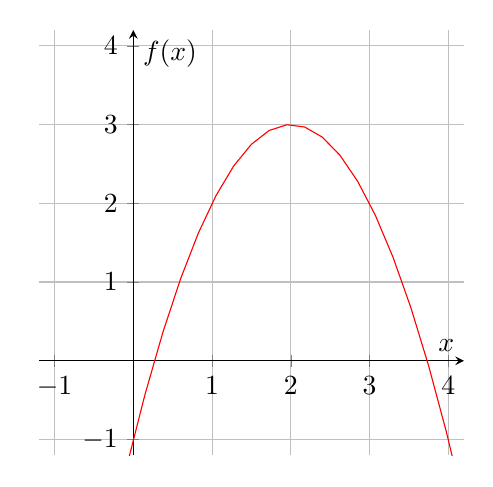
\begin{tikzpicture}
\begin{axis}[ axis x line=middle, axis y line=middle,xmax=4.2,ymax=4.2,xmin=-1.2,ymin=-1.2,ylabel=$f(x)$, xlabel=$x$, legend pos = north west,x=1cm,y=1cm,grid = major]
\addplot[domain= -1.2:4.2, color = red]{(-1)*x^2+4*x-1};
    \end{axis}
\end{tikzpicture}
\end{center}


对于上图的函数,根据函数的图像,当$x$越来越接近2的时候,函数值$f(x)$愈发接近\underline{\hbox to 5mm{}},所以我们可以写出:\[{\lim_{x\to 2}} f(x) = \underline{\hbox to 5mm{}}\]

在刚才那个函数中,我们可以发现x\underline{\hbox to 5mm{}}(可以/不可以)等于2,而函数等于2的时候,函数值$f(2)$恰好就是我们刚才所求的那个limit。这是一个巧合吗?我们可以把它写成:\[{\lim_{x\to 2}} f(x) = f(2)\]

那么是不是对于所有函数的所有点,我们都可以写出:\[{\lim_{x\to a}} f(x) = f(a)\]

来看一下下面这个例子:
\[f(x) =  \frac{x^2-1}{x-1}\]
函数的domain是$x\not= \underline{\hbox to 5mm{}}$

\begin{center}
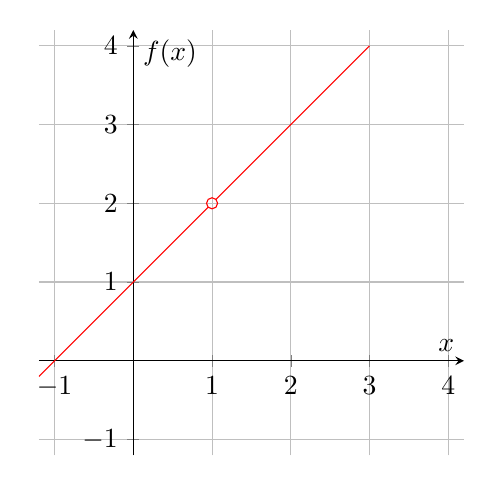
\begin{tikzpicture}
\begin{axis}[ axis x line=middle, axis y line=middle,xmax=4.2,ymax=4.2,xmin=-1.2,ymin=-1.2,ylabel=$f(x)$, xlabel=$x$, legend pos = north west,x=1cm,y=1cm,grid = major]
\addplot[domain= -1.2:0.95, color = red]{(x^2-1)/(x-1)};
\addplot+[only marks, mark = o] coordinates
{(1,2)};
\addplot[domain= 1.05:3, color = red]{(x^2-1)/(x-1)};
    \end{axis}
\end{tikzpicture}
\end{center}

通过图像,我们可以发现,当自变量$x$越接近于1时,函数值越接近于\underline{\hbox to 5mm{}}(数字)。因为domain的原因,$x$\underline{\hbox to 5mm{}}(可以/不可以)等于1。虽然$x$\underline{\hbox to 5mm{}}(可以/不可以)等于1,根据limit的定义,这对函数在$x=1$处的limit\underline{\hbox to 5mm{}}(有影响/不影响)。
所以,\[{\lim_{x\to 1}} \frac{x^2-1}{x-1} = \underline{\hbox to 5mm{}}\]
而\[f(1) = \underline{\hbox to 5mm{}}\]

所以我们可以知道\[{\lim_{x\to 1}} f(x) = f(2)\] (成立/不成立)

所以\[{\lim_{x\to a}} f(x) = f(a)\](永远成立/并非永远成立)

该公式何时成立?成立又意味着什么?我们到后面再来探讨。

\paragraph{发现}
我们把刚才的函数稍微变化一下,变成一个“人工制造”的函数:
\[f(x) = 
\begin{cases}
1 & x = 1\\
\frac{x^2-1}{x-1} & x\not=1
\end{cases}
\]

这样,函数图像可以就成了:

\begin{center}
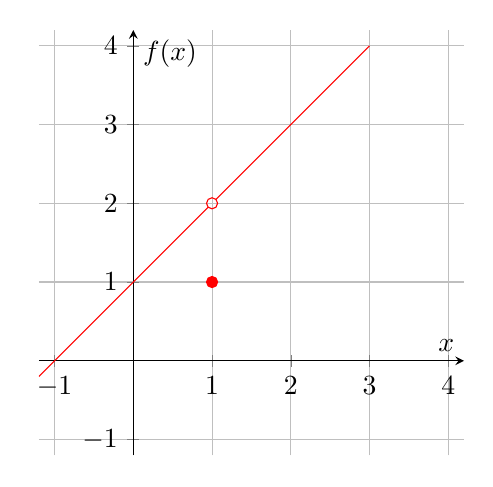
\begin{tikzpicture}
\begin{axis}[ axis x line=middle, axis y line=middle,xmax=4.2,ymax=4.2,xmin=-1.2,ymin=-1.2,ylabel=$f(x)$, xlabel=$x$, legend pos = north west,x=1cm,y=1cm,grid = major]
\addplot[domain= -1.2:0.95, color = red]{(x^2-1)/(x-1)};
\addplot+[only marks, mark = o] coordinates
{(1,2)};
\addplot[domain= 1.05:3, color = red]{(x^2-1)/(x-1)};
\addplot+[only marks, mark =*, color = red] coordinates
{(1,1)};
    \end{axis}
\end{tikzpicture}
\end{center}

\[{\lim_{x\to 1}} f(x) = \underline{\hbox to 5mm{}} \text {;} f(1) =\underline{\hbox to 5mm{}} \]

\paragraph{总结}
函数在$x=a$处的limit,与函数在$x=a$处是否有定义\underline{\hbox to 5mm{}}(有关/无关),与函数在$x=a$处的函数值大小\underline{\hbox to 5mm{}}(有关/无关)

\paragraph{发现}
通过图像,我们也能够更直观的找到函数在某一点的left-hand limit和函数在某一点的right-hand limit:

\begin{center}
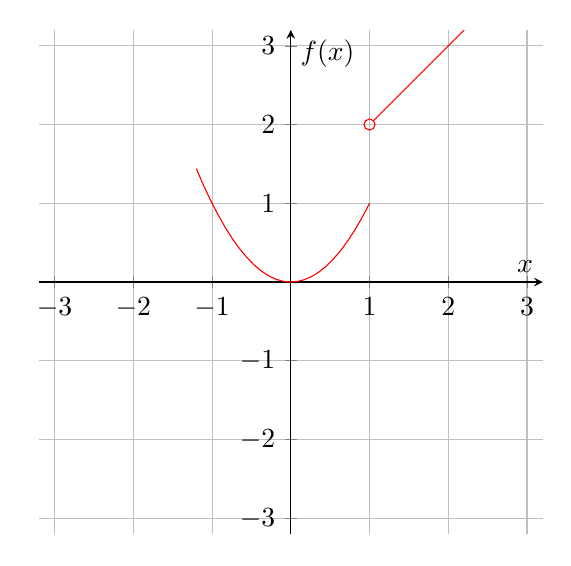
\begin{tikzpicture}
\begin{axis}[ axis x line=middle, axis y line=middle,xmax=3.2,ymax=3.2,xmin=-3.2,ymin=-3.2,ylabel=$f(x)$, xlabel=$x$, legend pos = north west,x=1cm,y=1cm,grid = major]
\addplot[domain= -1.2:1, color = red]{x^2};
\addplot+[only marks, mark = o] coordinates
{(1,2)};
\addplot[domain= 1.05:3, color = red]{(x^2-1)/(x-1)};
    \end{axis}
\end{tikzpicture}
\end{center}

对于函数$f(x)$而言,$f(1)=\underline{\hbox to 5mm{}}$(数字),如果从左边接近$x = 1$点,我们可以发现函数值趋近于\underline{\hbox to 5mm{}}(数字),这也意味着函数的\underline{\hbox to 5mm{}}(left-hand limit/ right-hand limit)是\underline{\hbox to 5mm{}}(数字)。

如果从右边接近$x = 1$点,我们可以发现函数值趋近于\underline{\hbox to 5mm{}}(数字),这也意味着函数的\underline{\hbox to 5mm{}}(left-hand limit/ right-hand limit)是\underline{\hbox to 5mm{}}(数字)。

函数的left-hand limit\underline{\hbox to 5mm{}}(等于/不等于)right-hand limit。

\paragraph{游戏}

\begin{center}
\begin{tikzpicture}
\begin{axis}[ axis x line=middle, axis y line=middle,xmax=3.2,ymax=3.2,xmin=-3.2,ymin=-3.2,ylabel=$f(x)$, xlabel=$x$, legend pos = north west,x=1cm,y=1cm]
\addplot[domain= -3:-0.05, color = red]{-1};
\addplot[domain= 0:1, color = red]{1};
\addplot[domain= 1:2, color = red]{x};
\addplot[domain= 2:3, color = red]{2};
\addplot+[only marks, mark = o,color = red] coordinates
{(0,-1)};
    \end{axis}
\end{tikzpicture}
\end{center}

如果从左边接近$x = 0$点,我们可以发现函数值趋近于\underline{\hbox to 5mm{}}(数字),这也意味着函数的\underline{\hbox to 5mm{}}(left-hand limit/ right-hand limit)是\underline{\hbox to 5mm{}}(数字)。

如果从右边接近$x = 2$点,我们可以发现函数值趋近于\underline{\hbox to 5mm{}}(数字),这也意味着函数的\underline{\hbox to 5mm{}}(left-hand limit/ right-hand limit)是\underline{\hbox to 5mm{}}(数字)。

\begin{center}
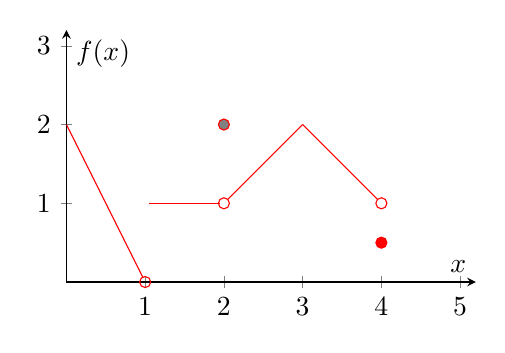
\begin{tikzpicture}
\begin{axis}[ axis x line=middle, axis y line=middle,xmax=5.2,ymax=3.2,xmin=0,ymin=0,ylabel=$f(x)$, xlabel=$x$, legend pos = north west,x=1cm,y=1cm]
\addplot[domain= 0:0.97, color = red]{-2*x+2};
\addplot[domain= 1.05:1.95, color = red]{1};
\addplot[domain= 2.05:3, color = red]{x-1};
\addplot[domain= 3:3.95, color = red]{-x+5};
\addplot+[only marks, mark = o,color = red] coordinates
{(1,0)};
\addplot+[only marks, mark = o,color = red] coordinates
{(2,1)};
\addplot+[only marks, mark = o,color = red] coordinates
{(4,1)};
\addplot+[only marks, mark = *,color = red] coordinates
{(2,2)};
\addplot+[only marks, mark = *,color = red] coordinates
{(4,0.5)};
    \end{axis}
\end{tikzpicture}
\end{center}

如果从左边接近$x = 0$点,我们可以发现函数值趋近于\underline{\hbox to 5mm{}}(数字),这也意味着函数的\underline{\hbox to 5mm{}}(left-hand limit/ right-hand limit)是\underline{\hbox to 5mm{}}(数字)。

如果从右边接近$x = 0$点,我们可以发现函数值趋近于\underline{\hbox to 5mm{}}(数字),这也意味着函数的\underline{\hbox to 5mm{}}(left-hand limit/ right-hand limit)是\underline{\hbox to 5mm{}}(数字)。

如果从左边接近$x = 1$点,我们可以发现函数值趋近于\underline{\hbox to 5mm{}}(数字),这也意味着函数的\underline{\hbox to 5mm{}}(left-hand limit/ right-hand limit)是\underline{\hbox to 5mm{}}(数字)。

如果从右边接近$x = 1$点,我们可以发现函数值趋近于\underline{\hbox to 5mm{}}(数字),这也意味着函数的\underline{\hbox to 5mm{}}(left-hand limit/ right-hand limit)是\underline{\hbox to 5mm{}}(数字)。

如果从左边接近$x = 2$点,我们可以发现函数值趋近于\underline{\hbox to 5mm{}}(数字),这也意味着函数的\underline{\hbox to 5mm{}}(left-hand limit/ right-hand limit)是\underline{\hbox to 5mm{}}(数字)。

如果从右边接近$x = 2$点,我们可以发现函数值趋近于\underline{\hbox to 5mm{}}(数字),这也意味着函数的\underline{\hbox to 5mm{}}(left-hand limit/ right-hand limit)是\underline{\hbox to 5mm{}}(数字)。

如果从左边接近$x = 3$点,我们可以发现函数值趋近于\underline{\hbox to 5mm{}}(数字),这也意味着函数的\underline{\hbox to 5mm{}}(left-hand limit/ right-hand limit)是\underline{\hbox to 5mm{}}(数字)。

如果从右边接近$x = 3$点,我们可以发现函数值趋近于\underline{\hbox to 5mm{}}(数字),这也意味着函数的\underline{\hbox to 5mm{}}(left-hand limit/ right-hand limit)是\underline{\hbox to 5mm{}}(数字)。

如果从左边接近$x = 4$点,我们可以发现函数值趋近于\underline{\hbox to 5mm{}}(数字),这也意味着函数的\underline{\hbox to 5mm{}}(left-hand limit/ right-hand limit)是\underline{\hbox to 5mm{}}(数字)。

如果从右边接近$x = 4$点,我们可以发现函数值趋近于\underline{\hbox to 5mm{}}(数字),这也意味着函数的\underline{\hbox to 5mm{}}(left-hand limit/ right-hand limit)是\underline{\hbox to 5mm{}}(数字)。

\subsubsection{Does the Limit exist?}
\paragraph{探索}
函数在任何一点处的limit或者函数在无穷大/无穷小处的limit是永远存在的吗?我们下面来探讨这个问题:
请尝试求出以下limit:
\[{\lim_{x\to +\infty }} \sin{x} = ?\]

\begin{center}
\begin{tabular}{c|c|c|c|c}
\hline
$x$  & 1 & 10 &100& 1000 \\
\hline
$\sin{x}$ & &  &  & \\
\hline
\end{tabular}
\end{center}
我们可以发现,在$x$趋近于无穷大时,函数的取值是\underline{\hbox to 5mm{}}(有规律/无规律的),我们可以推测这可能是由于函数的\underline{\hbox to 5mm{}}决定的。

\paragraph{发现}
函数的周期性在一般情况下只会导致在$\infty$或者$-\infty$的时候极限不存在,但是在某些特殊情况下,也会导致在$x = 0$处不存在极限。
\[f(x) = 
\begin{cases}
0 & x = 0\\
\sin{\frac{1}{x}} & x\not=1
\end{cases}
\]

这个函数的图像长这个样子:
\begin{center}
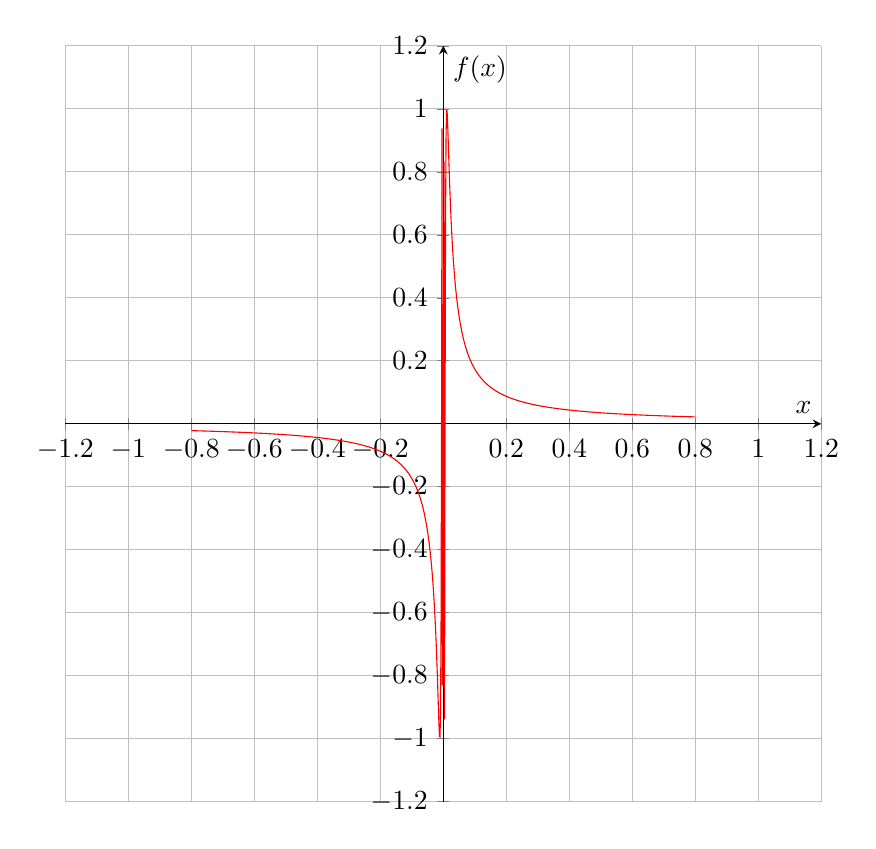
\begin{tikzpicture}
\begin{axis}[ axis x line=middle, axis y line=middle,xmax=1.2,ymax=1.2,xmin=-1.2,ymin=-1.2,ylabel=$f(x)$, xlabel=$x$, legend pos = north west,x=4cm,y=4cm,grid = major]
\addplot[domain= -0.8:0.8, color = red, samples = 1000]{sin(1/x)};
    \end{axis}
\end{tikzpicture}
\end{center}

这张图我们很难看出来什么,那么我们再把它放大一些:

\begin{center}
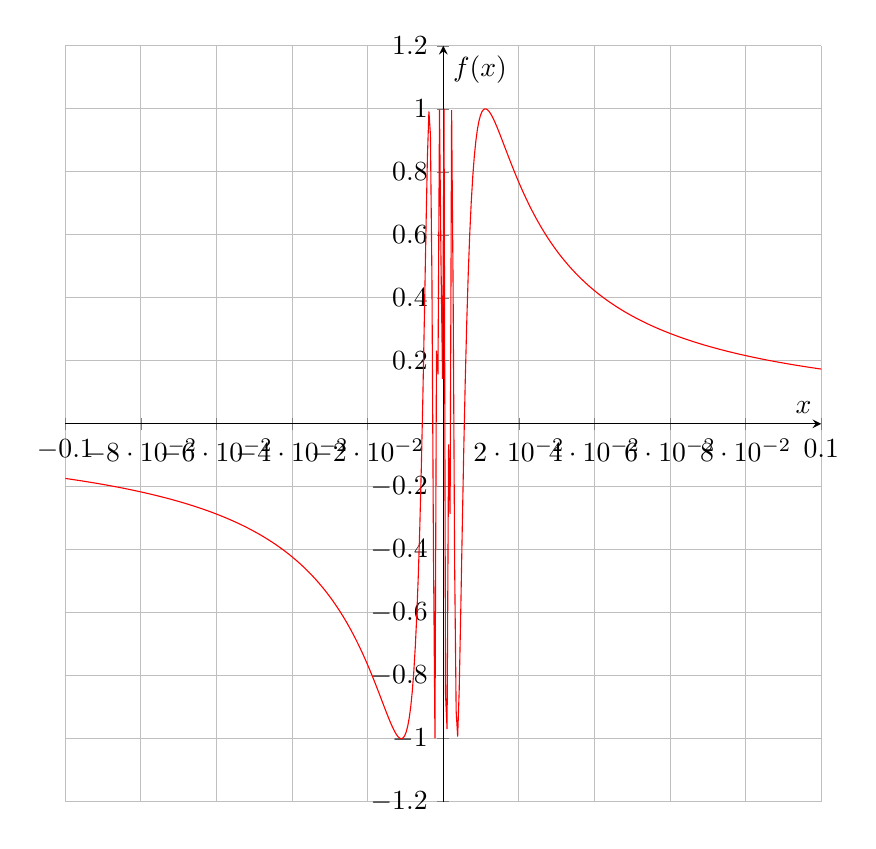
\begin{tikzpicture}
\begin{axis}[ axis x line=middle, axis y line=middle,xmax=0.1,ymax=1.2,xmin=-0.1,ymin=-1.2,ylabel=$f(x)$, xlabel=$x$, legend pos = north west,x=48cm,y=4cm,grid = major]
\addplot[domain= -0.2:0.2, color = red, samples = 1000]{sin(1/x)};
    \end{axis}
\end{tikzpicture}
\end{center}

好像还是看不出来?继续放大

\begin{center}
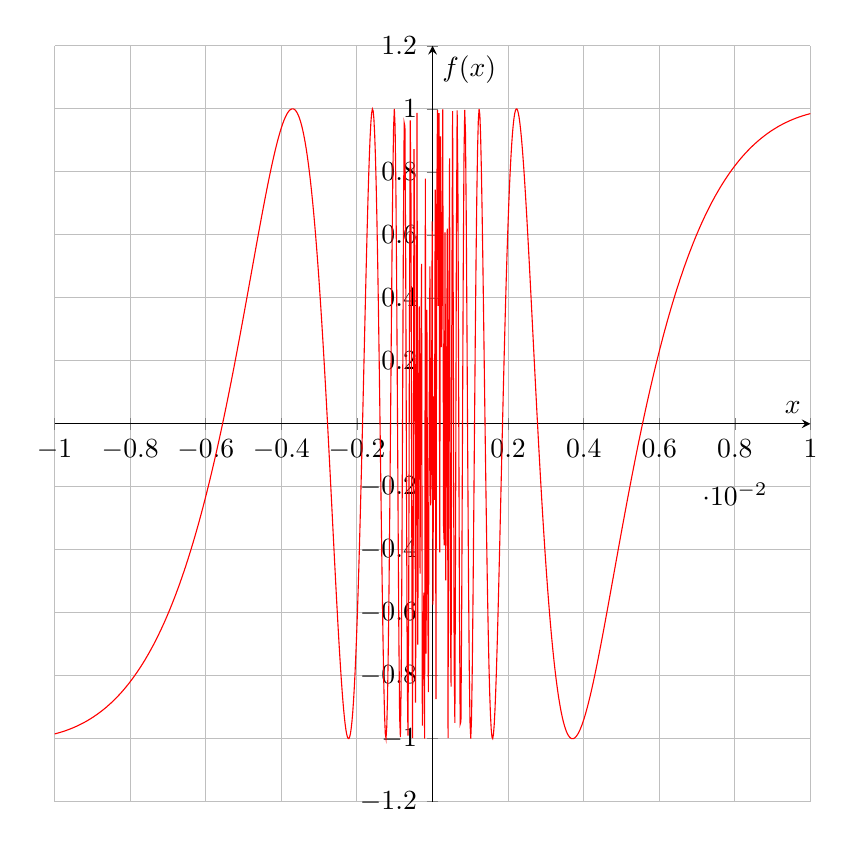
\begin{tikzpicture}
\begin{axis}[ axis x line=middle, axis y line=middle,xmax=0.01,ymax=1.2,xmin=-0.01,ymin=-1.2,ylabel=$f(x)$, xlabel=$x$, legend pos = north west,x=480cm,y=4cm,grid = major]
\addplot[domain= -0.01:0.01, color = red, samples = 1000]{sin(1/x)};
    \end{axis}
\end{tikzpicture}
\end{center}

是不是越来越乱了?没错,这个函数越靠近0的地方,上下起伏波动的就越\underline{\hbox to 5mm{}}(频繁/不频繁),像这样的函数,很难说清在$x = 0$处的limit究竟是几。

\paragraph{总结}
在所求位置附近,若函数值在不断、频繁的上下波动,则该位置不存在limit。

\paragraph{游戏}
判断以下函数在所求的位置处是否存在limit?
\[{\lim_{x\to +\infty }} -\cos{2x} \]
\[{\lim_{x\to 0 }} -\tan{2x} \]
\[{\lim_{x\to -\infty }} exp{2x} \]
\[{\lim_{x\to 2 }} 2\sin{x}\cos{x} \]
\[{\lim_{x\to 0 }} |x| \]
\[{\lim_{x\to 0 }} \frac{x}{|x|} \]

\paragraph{发现}
观察如下函数在$x=0$ , $ x = 1$ 以及 $x = 2$处的极限:

\begin{center}
\begin{tikzpicture}
\begin{axis}[ axis x line=middle, axis y line=middle,xmax=5.2,ymax=5.2,xmin=-5.2,ymin=0,ylabel=$f(x)$, xlabel=$x$, legend pos = north west,x=1cm,y=1cm]
\addplot[domain= -4:0, color = red]{-x};
\addplot[domain= 0:0.95, color = red]{x};
\addplot[domain= 1.05:1.95, color = red]{x};
\addplot[domain= 2.05:4, color = red]{x^2-1};
\addplot+[only marks, mark = o,color = red] coordinates
{(1,1)};
\addplot+[only marks, mark = o,color = red] coordinates
{(2,2)};
\addplot+[only marks, mark = *,color = red] coordinates
{(1,3)};
    \end{axis}
\end{tikzpicture}
\end{center}

\[{\lim_{x\to 0^- }} f(x) = \underline{\hbox to 5mm{}}\text{(数字)}\]
\[{\lim_{x\to 0^+ }} f(x) = \underline{\hbox to 5mm{}}\text{(数字)}\]
\[{\lim_{x\to 0^- }} f(x) = \underline{\hbox to 5mm{}}\text{(等于/不等于)}{\lim_{x\to 0^+ }} f(x) \]

\[{\lim_{x\to 1^- }} f(x) = \underline{\hbox to 5mm{}}\text{(数字)}\]
\[{\lim_{x\to 1^+ }} f(x) = \underline{\hbox to 5mm{}}\text{(数字)}\]
\[{\lim_{x\to 1^- }} f(x) = \underline{\hbox to 5mm{}}\text{(等于/不等于)}{\lim_{x\to 1^+ }} f(x) \]

\[{\lim_{x\to 2^- }} f(x) = \underline{\hbox to 5mm{}}\text{(数字)}\]
\[{\lim_{x\to 2^+ }} f(x) = \underline{\hbox to 5mm{}}\text{(数字)}\]
\[{\lim_{x\to 2^- }} f(x) = \underline{\hbox to 5mm{}}\text{(等于/不等于)}{\lim_{x\to 2^+ }} f(x) \]

如果在$x = a$处 left-hand limit 和 right-hand limit 均存在且 left-hand limit 等于 right-hand limit,我们就可以非常自信的告诉大家,function $f(x)$ has a limit at $x = a$。

如果在$x = a$处 left-hand limit 和 right-hand limit 不存在,或者 left-hand limit 不等于 right-hand limit,我们只能遗憾的告诉大家 function $f(x)$ does not has a limit at $x = a$。

\paragraph{注意}
“limit exsits”和“函数在该处有定义”是无关的,函数没有定义的地方也可以存在limit。 

\subsubsection{章节小结}

\paragraph{Definition of Limits}
如果在$x$不断接近$a$的时候($a$可以在,也可以不在$f(x)$的定义域中),函数值$f(x)$不断接近于某个数$L$。我们说$L$就是在$x$趋近于$a$时函数$f(x)$的\textcolor{red}{极限};If $f(x)$ gets arbitrarily close to $L$, for all $x$ sufficiently close to $a$, we say that $f(x)$ approaches the\textcolor{red}{limit} $L$ as x approaches $a$, and we write:
\[{\lim_{x\to a }} f(x) = L\]

\paragraph{Left-hand limit and right-hand limit}
 如果$x$从左边靠近$a$,这样的得到的limit,我们管它叫做\textcolor{red}{left-hand limit},并且可以表示为:
\[ {\lim_{x\to a^- }} f(x) = L\]
a右上角的负号可以理解为“函数值x从负方向逼近a”

We write \[ {\lim_{x\to a^- }} f(x) = L\]

and say the \textcolor{red}{left-hand limit} of $f(x)$ as $x$ approaches $a$ is equal to $L$.

如果$x$从右边靠近$a$,这样的得到的limit,我们管它叫做\textcolor{red}{left-hand limit},并且可以表示为:
\[ {\lim_{x\to a^+ }} f(x) = L\]
a右上角的正号可以理解为“函数值x从正方向逼近a”

We write \[ {\lim_{x\to a^+ }} f(x) = L\]

and say the \textcolor{red}{right-hand limit} of $f(x)$ as $x$ approaches $a$ is equal to $L$.

\paragraph{Existence of Limits}
目前我们有两种办法判定limit不存在:

1. 在所求位置附近,若函数值在不断、频繁的上下波动,则该位置不存在limit。

2. 若在$x = a$处 $ {\lim_{x\to a^- }} f(x) \not = {\lim_{x\to a^+ }}  f(x) $,则$x=a $处不存在limit。

\subsection{Calculating Limits Algebraically: First Approach}
\subsubsection{The Limit Laws}
\paragraph{发现}
在上一章节中,我们猜测函数的极限主要靠“蒙”。但是“蒙”不一定是准确的,在很多情况下是“懵逼”的,例如...
\[f(x) = x^3 + \frac{cos(5x)}{10000}\]
\begin{center}
\begin{tabular}{c|c|c|c|c}
\hline
$x$  & 1 & 0.5 & 0.1& 0.05 \\
\hline
$f(x)$ & 1.000 & 0.125 & 0.001 & 0.0002\\
\hline
\end{tabular}
\end{center}

这个表格很容易让我们大家得出结论:\[{\lim_{x\to 0}} f(x) = 0\]
然而请稍等,如果我们再向0靠的更近一些,就能看到...

\begin{center}
\begin{tabular}{c|c|c|c}
\hline
$x$  & 0.01 & 0.005 & 0.001 \\
\hline
$f(x)$ & 0.000101 & 0.00010009 & 0.00010000 \\
\hline
\end{tabular}
\end{center}

好吧,这下答案呼之欲出了,并不是\[{\lim_{x\to 0}} f(x) = 0\]而是\[{\lim_{x\to 0}} f(x) = 0.0001\]

这呼吁我们使用一些更靠谱的方式去研究函数的极限。

\paragraph{探索}
常数函数是最简单的函数:\[ f(x) = A \text{, where A is a constant real number} \]

我们可以画出常数函数的图像,根据图像,可以知道:

\[{\lim_{x\to a }} f(x) = \underline{\hbox to 5mm{}}\text{(字母)}\]

即常数函数在任意一点的极限都是常数函数本身。

\paragraph{游戏}
求下列函数的极限:
\[ {\lim_{x \to 3} 5 }\]
\[ {\lim_{x \to -4} 5 }\]
\[ {\lim_{x \to 0} 5 }\]
\[ {\lim_{x \to 0} e }\]
\[ {\lim_{x \to \pi} 0 }\]

\paragraph{发现}
所有简单的初等函数在domain(定义域)中某一点的极限,都可以用将该点坐标带入函数得出,这些初等函数包括:
\[\text{幂函数 } {\lim_{x \to b} x^n} = b^n \]
\[\text{指数函数 } {\lim_{x \to b} a^x} = a^b \]
\[\text{对数函数 } {\lim_{x \to b} log_ax} = log_ab \]
\[\text{三角函数 } {\lim_{x \to b} \sin{x}} = \sin{b} \]

\paragraph{定理}
Suppose that a,b, c are constants and the limits
\[{\lim_{x \to a} f(x)} \qquad \text{and} \qquad {\lim_{x \to a} g(x)}\]
exist. Then:
\[\text{Sum Rule }\qquad {\lim_{x \to a} [f(x) + g(x)]} = {\lim_{x \to a} f(x)}+{\lim_{x \to a} g(x)}\]
\[\text{Difference Rule }\qquad {\lim_{x \to a} [f(x) - g(x)]} = {\lim_{x \to a} f(x)}-{\lim_{x \to a} g(x)}\]
\[\text{Product Rule }\qquad {\lim_{x \to a} [f(x) \cdot g(x)]} = {\lim_{x \to a} f(x)} \cdot {\lim_{x \to a} g(x)}\]
\[\text{Quotient Rule }\qquad {\lim_{x \to a} \frac{f(x)}{g(x)}} =\frac{{\lim_{x \to a} f(x)}}{{\lim_{x \to a} g(x)}}\]
\[\text{Power Rule }\qquad {\lim_{x \to a} (f(x))^{b/c}} = ({\lim_{x \to a} f(x)})^{b/c}\]

\paragraph{游戏}

(Sum Rule)
\[ {\lim_{x \to 2} x^3 + x} = {\lim_{x \to 2} x^3} + {\lim_{x \to 2} \underline{\hbox to 5mm{}}} =  \underline{\hbox to 5mm{}} + \underline{\hbox to 5mm{}} =  \underline{\hbox to 5mm{}}\]
\[ {\lim_{x \to -\pi} \sin{x} + \cos{x}} = {\lim_{x \to -\pi} \underline{\hbox to 5mm{}}} + {\lim_{x \to -\pi} \underline{\hbox to 5mm{}}} =  \underline{\hbox to 5mm{}} + \underline{\hbox to 5mm{}} =  \underline{\hbox to 5mm{}}\]
\[ {\lim_{x \to 0} 2^x + 2^{-x}} = {\lim_{x \to 0} \underline{\hbox to 5mm{}}} + {\lim_{x \to 0} \underline{\hbox to 5mm{}}} =  \underline{\hbox to 5mm{}} + \underline{\hbox to 5mm{}} =  \underline{\hbox to 5mm{}}\]

(Difference Rule)
\[ {\lim_{x \to 0} x^2 - e^x} = {\lim_{x \to 0} x^2} - {\lim_{x \to 0} \underline{\hbox to 5mm{}}} =  \underline{\hbox to 5mm{}} - \underline{\hbox to 5mm{}} =  \underline{\hbox to 5mm{}}\]
\[ {\lim_{x \to -3} 5x - 6} = {\lim_{x \to -3} \underline{\hbox to 5mm{}}} + {\lim_{x \to -3} \underline{\hbox to 5mm{}}} =  \underline{\hbox to 5mm{}} - \underline{\hbox to 5mm{}} =  \underline{\hbox to 5mm{}}\]
\[ {\lim_{x \to \frac{\pi}{4}} \tan{x} - \cos{x}} = {\lim_{x \to \frac{\pi}{4}} \underline{\hbox to 5mm{}}} + {\lim_{x \to \frac{\pi}{4}} \underline{\hbox to 5mm{}}} =  \underline{\hbox to 5mm{}} - \underline{\hbox to 5mm{}} =  \underline{\hbox to 5mm{}}\]

(Product Rule)
\[ {\lim_{x \to -1} x \cdot e^x} = {\lim_{x \to -1} x} \cdot {\lim_{x \to -1} \underline{\hbox to 5mm{}}} =  \underline{\hbox to 5mm{}} \cdot \underline{\hbox to 5mm{}} =  \underline{\hbox to 5mm{}}\]
\[ {\lim_{x \to a} 2^x \cdot x^2 } = {\lim_{x \to a} \underline{\hbox to 5mm{}}} \cdot {\lim_{x \to a} \underline{\hbox to 5mm{}}} =  \underline{\hbox to 5mm{}} \cdot \underline{\hbox to 5mm{}} =  \underline{\hbox to 5mm{}}\]
\[ {\lim_{x \to 4} 3 \cdot x^2} = {\lim_{x \to 4} \underline{\hbox to 5mm{}}} \cdot {\lim_{x \to 4} \underline{\hbox to 5mm{}}} =  \underline{\hbox to 5mm{}} \cdot \underline{\hbox to 5mm{}} =  \underline{\hbox to 5mm{}}\]

(Quotient Rule)
\[ {\lim_{x \to \frac{\pi}{2}} \frac{\sin{x}}{x}} = \frac{{\lim_{x \to \frac{\pi}{2}} \sin{x}}}{{\lim_{x \to \frac{\pi}{2}} \underline{\hbox to 5mm{}}}} =  \frac{\underline{\hbox to 5mm{}}}{\underline{\hbox to 5mm{}}} =  \underline{\hbox to 5mm{}}\]
\[ {\lim_{x \to 0} \frac{4^x}{3}} = \frac{{\lim_{x \to 0} \underline{\hbox to 5mm{}}}}{{\lim_{x \to 0} \underline{\hbox to 5mm{}}}} =  \frac{\underline{\hbox to 5mm{}}}{\underline{\hbox to 5mm{}}} =  \underline{\hbox to 5mm{}}\]
\[ {\lim_{x \to -2} \frac{x^2}{\sqrt{x}}} = \frac{{\lim_{x \to -2} \underline{\hbox to 5mm{}}}}{{\lim_{x \to -2} \underline{\hbox to 5mm{}}}} =  \frac{\underline{\hbox to 5mm{}}}{\underline{\hbox to 5mm{}}} =  \underline{\hbox to 5mm{}}\]

(Power Rule)
\[ {\lim_{x \to \pi} \cos^3{x}} = ({\lim_{x \to \pi} \cos{x}})^3 =  (\underline{\hbox to 5mm{}})^3 =  \underline{\hbox to 5mm{}}\]
\[ {\lim_{x \to 0} (2^x)^4} = ({\lim_{x \to 0} \underline{\hbox to 5mm{}}})^4 =  (\underline{\hbox to 5mm{}})^4 =  \underline{\hbox to 5mm{}}\]
\[ {\lim_{x \to \pi} \sqrt[3]{\cos{x}}} = \sqrt[3]{{\lim_{x \to \pi} \underline{\hbox to 5mm{}}}} =  \sqrt[3]{\underline{\hbox to 5mm{}}} =  \underline{\hbox to 5mm{}}\]
\[ {\lim_{x \to 0} \sqrt[4]{2^x}} = \sqrt[4]{{\lim_{x \to 0} \underline{\hbox to 5mm{}}}} =  \sqrt[4]{\underline{\hbox to 5mm{}}} =  \underline{\hbox to 5mm{}}\]
\[ {\lim_{x \to 8} \sqrt[5]{x^2}} = \sqrt[5]{\lim_{x \to 8} \underline{\hbox to 5mm{}}} =  \sqrt[5]{\underline{\hbox to 5mm{}}} =  \underline{\hbox to 5mm{}}\]

(主线任务)
\begin{eqnarray*}
{\lim_{x \to 4} (2x^2 - 3x + 1)} \\
& = & {\lim_{x \to 4} \underline{\hbox to 5mm{}}} - {\lim_{x \to 4} \underline{\hbox to 5mm{}}} + {\lim_{x \to 4} \underline{\hbox to 5mm{}}}\\
{\lim_{x \to 4} 2x^2} = \underline{\hbox to 5mm{}} ; {\lim_{x \to 4} 3x} = \underline{\hbox to 5mm{}}; {\lim_{x \to 4} 1} = \underline{\hbox to 5mm{}}\\
\text{Therefore,} {\lim_{x \to 4} 2x^2 - 3x + 1}  = \underline{\hbox to 5mm{}} - \underline{\hbox to 5mm{}} + \underline{\hbox to 5mm{}}\\
& = & \underline{\hbox to 5mm{}}
\end{eqnarray*}

\begin{eqnarray*}
{\lim_{x \to \pi} \frac{(\sin{x} + \cos{x} - x^2) \cdot 3x}{\sqrt{x}}} \\
& = & \frac{({\lim_{x \to \pi} \underline{\hbox to 5mm{}}} + {\lim_{x \to \pi}\underline{\hbox to 5mm{}}} - {\lim_{x \to \pi} \underline{\hbox to 5mm{}}} )\cdot {\lim_{x \to \pi} \underline{\hbox to 5mm{}}}}{{\lim_{x \to \pi} \underline{\hbox to 5mm{}}}}\\
& = & \frac{(\underline{\hbox to 5mm{}}-\underline{\hbox to 5mm{}}+\underline{\hbox to 5mm{}}) \cdot \underline{\hbox to 5mm{}}}{\underline{\hbox to 5mm{}}}\\
& = & \frac{\underline{\hbox to 5mm{}}}{\underline{\hbox to 5mm{}}}
\end{eqnarray*}

\paragraph{总结}
根据Limit Laws,只要函数是上面列出的初等函数或者初等函数的组合(加、减、乘、除、乘方、开方),函数在某一点的limit可以通过把$x$直接带入函数式求得。这么做的前提是,函数在所求点必须\textcolor{red}{有定义}。
以下三个limit就可以直接把$x$带入函数式求得:
\[ {\lim_{x \to 4} x } \text{;} {\lim_{x \to 0} \sin x} \text{;} {\lim_{x \to 2} (5x-3)}\]
对于以下三个limit,函数在所求点并没有定义,所以不能把$x$直接带入求解:
\[ {\lim_{x \to 0} \frac{1}{x} } \text{;} {\lim_{x \to 1} \frac {x^2-1}{x-1}} \text{;} {\lim_{x \to 1} \sqrt{x^2-4}}\]

\paragraph{探索}
在将来求Limits的时候,我们会经常和$\infty$这个符号打交道,$\infty$读作''Infinity''(无穷)。“无穷”是什么意思呢?可以非常简单的理解为,$\infty$的意思就是,你脑子中随便想一个数字,而$\infty$一定比你想的这个数字要大。

就是说“要多大有多大”。

$10^{100}$够大了吧?$\infty$比你还大。

$1000^{1000}$呢?也还是不如$\infty$。

这就是$\infty$的含义。一定要注意,$\infty$并不是一个数,而是一个“概念”。我们可以参照${\lim_{x \to 0^+} \frac{1}{x}}$来说明这一点:这个极限的意思是,当$x$从右侧靠近$x=0$的时候,函数值$f(x)$会趋向于多少。我们可以列一个表:

\begin{center}
\begin{tabular}{c|c|c|c|c}
\hline
$x$  & 0.1 & 0.01 & 0.001& 0.0001 \\
\hline
$f(x)$ & 10 & 100 & 1000 & 10000\\
\hline
\end{tabular}
\end{center}

可以看出来,随着$x$不断向$0$接近,$f(x)$的数值是上不封顶的,也就是说,\textcolor{red}{你随便说一个数,在$x$小于某个值的时候,$f(x)$一定会比你说的那个数更大}。

严谨的来说,对于我随便说的数$\varepsilon$,总有一个这么数$\delta$存在,使得当$0<x<\delta$的时候$f(x) > \varepsilon$,那么我就可以说${\lim_{x \to 0+} f(x)} = \infty$

如果我随便说的数是100,当$0<x<\underline{\hbox to 5mm{}}$时,$f(x) > 100$ ;在这个例子中,$\varepsilon = \underline{\hbox to 5mm{}}$,$\delta=\underline{\hbox to 5mm{}}$

如果我随便说的数是500,当$x<\underline{\hbox to 5mm{}}$时,$f(x) > 500$ ;在这个例子中,$\varepsilon = \underline{\hbox to 5mm{}}$,$\delta=\underline{\hbox to 5mm{}}$

如果我随便说的数是$10^200$,当$x<\underline{\hbox to 5mm{}}$时,$f(x) > 10^200$ ;在这个例子中,$\varepsilon = \underline{\hbox to 5mm{}}$,$\delta=\underline{\hbox to 5mm{}}$

\paragraph{发现}
尽管严谨的来说,$\infty$与$-\infty$并不是数字,我们依然可以在求limit的时候将其视为数字,带入函数求limit。在这么做的时候,只需要注意:
\[ \frac{1}{0} = \infty \]
\[\frac{1}{\infty} = 0 \]
用这种方法,我们可以求${\lim_{x \to 0} \frac{1}{x^2}}$ :
\[{\lim_{x \to 0} \frac{1}{x^2} = \frac{1}{0 ^ 2} = \frac{1}{0} = \infty} \]
 \[{\lim_{x \to 0} -\frac{1}{\sqrt{x}}} = \frac{\underline{\hbox to 5mm{}}}{\underline{\hbox to 5mm{}}} = \underline{\hbox to 5mm{}} \]
\[{\lim_{x \to 0} 3+\frac{1}{x} = 3+ \frac{1}{\underline{\hbox to 5mm{}}} = 3+\underline{\hbox to 5mm{}} = \underline{\hbox to 5mm{}}} \]

\paragraph{游戏}
用“代入法”求以下函数的Limit,注意有些Limit涉及$\infty$
\[ {\lim_{x \to 2} 2x } \text{;} {\lim_{x \to 0} 2x} \text{;} {\lim_{x \to \frac{1}{2}} (2x-1)}\]
\[ {\lim_{x \to 1} \frac{-1}{2x-1} } \text{;} {\lim_{x \to -1} 2x(3x-1)} \text{;} {\lim_{x \to -1} \frac{3x^2}{2x-1}}\]
\[ {\lim_{x \to \frac{\pi}{2}} x\sin{x} } \text{;} {\lim_{x \to \pi} \frac{\cos{x}}{1-\pi}} \text{;} {\lim_{x \to 1} \frac{x^3-1}{\sqrt{x} - 1}}\]
\[ {\lim_{x \to c} \frac{m_0}{\sqrt{1-\frac{v^2}{c^2}}} } \text{;} {\lim_{x \to \frac{2}{\pi}} \sin{\frac{1}{x}}} \text{;} {\lim_{x \to 3} \ln{(x^2-9)}}\]

\paragraph{总结}
总的来说,以下情况的limit都可以通过代入数字求得:

1. Limits of Polynomials(多项式函数的极限)
\[\text{If} f(x) = a_nx^n + a_{n-1}x^{n-1}+\cdots+a_0 \text{, then} {\lim_{x \to a} f(x) = f(a) = a_nc^n + a_{n-1}c^{n-1}+\ldots+a_0}\]
2. Limits of Rational Functions as long as the limit of denominator is non-zero(有理函数的极限,只要分母的极限不为0)
\[\text{If } f(x) \text{ and } g(x) \text{ are polynomials, then } {\lim_{x \to a} \frac{f(x)}{g(x)} = \frac{f(a)}{g(a)}} \text{ iff } g(a) \not = 0 \]

\subsubsection{Calculating One-Side Limits Algebraically}
\paragraph{发现}
当Left-hand Limit 和 Right-hand Limit 相等时,我们不需要做过多的干涉,直接将数字代入进公式就好,比如
\[{\lim_{x \to 2^+} x^2} = {\lim_{x \to 2^-} x^2} = 2^2 = 4\]
但是当Left-hand Limit不等于 Right-hand Limit时,我们就需要做一些小小的处理了。下面的问题是:怎么能知道某点的Left-hand Limit不等于Right-hand Limit呢?

\begin{center}
\begin{tikzpicture}
\begin{axis}[ axis x line=middle, axis y line=middle,xmax=5.2,ymax=5.2,xmin=-5.2,ymin=0,ylabel=$f(x)$, xlabel=$x$, legend pos = north west,x=1cm,y=1cm]
\addplot[domain= -4:0, color = red]{-x};
\addplot[domain= 0:0.95, color = red]{x};
\addplot[domain= 1.05:1.95, color = red]{x};
\addplot[domain= 2.05:4, color = red]{x^2-1};
\addplot+[only marks, mark = o,color = red] coordinates
{(1,1)};
\addplot+[only marks, mark = o,color = red] coordinates
{(2,2)};
\addplot+[only marks, mark = *,color = red] coordinates
{(1,3)};
    \end{axis}
\end{tikzpicture}
\end{center}

\[{\lim_{x\to 0^- }} f(x) = \underline{\hbox to 5mm{}}\text{(数字)}\]
\[{\lim_{x\to 0^+ }} f(x) = \underline{\hbox to 5mm{}}\text{(数字)}\]
\[{\lim_{x\to 0^- }} f(x) = \underline{\hbox to 5mm{}}\text{(等于/不等于)}{\lim_{x\to 0^+ }} f(x) \]
函数在这一点是\underline{\hbox to 5mm{}}(连续/续断/跳跃式中断)的

\[{\lim_{x\to 1^- }} f(x) = \underline{\hbox to 5mm{}}\text{(数字)}\]
\[{\lim_{x\to 1^+ }} f(x) = \underline{\hbox to 5mm{}}\text{(数字)}\]
\[{\lim_{x\to 1^- }} f(x) = \underline{\hbox to 5mm{}}\text{(等于/不等于)}{\lim_{x\to 1^+ }} f(x) \]
函数在这一点是\underline{\hbox to 5mm{}}(连续/续断/跳跃式中断)的

\[{\lim_{x\to 2^- }} f(x) = \underline{\hbox to 5mm{}}\text{(数字)}\]
\[{\lim_{x\to 2^+ }} f(x) = \underline{\hbox to 5mm{}}\text{(数字)}\]
\[{\lim_{x\to 2^- }} f(x) = \underline{\hbox to 5mm{}}\text{(等于/不等于)}{\lim_{x\to 2^+ }} f(x) \]
函数在这一点是\underline{\hbox to 5mm{}}(连续/续断/跳跃式中断)的

可以总结:当函数的图像在某点\underline{\hbox to 5mm{}}(连续/续断/跳跃式中断)的时候,我们就可以说这一点函数的Left-hand Limit不等于函数的Right-hand Limit,而满足这种“跳跃式中断”的函数,一般有三种:

1. 分式函数,例如$f(x) = \frac{1}{x}$在$x=0$点处。

2. $x$带有绝对值的函数,例如$f(x) = \frac{|x|}{x}$ 在$x=0$点处

3. “人工制造”的分段函数,例如
\[f(x) = 
\begin{cases}
x & x < 2\\
x^2 & x\geq2
\end{cases}
\]

【链接:关于连续部分的详细讨论,请参见后续连续章节】

\paragraph{发现}
现在残留的问题就是:如何不看图像就可以分别计算出这种“跳跃式中断”点的Right-hand和Left-hand Limit呢?
\[{\lim_{x \to 0^+} \frac{|x|}{x}}\]
当我们从0的正方向接近0的时候,$x$的值一直保持为$x\underline{\hbox to 5mm{}}(>/</=)0$

当$x>0$时,$|x| = \underline{\hbox to 5mm{}}$

根据这一定义,我们可以脱掉绝对值符号,原式变为:
\[{\lim_{x \to 0^+} \frac{x}{x}} = \underline{\hbox to 5mm{}}\] 

\[{\lim_{x \to 0^+} \frac{|x|}{x}}\]

当我们从0的负方向接近0的时候,$x$的值一直保持为$x\underline{\hbox to 5mm{}}(>/</=)0$

当$x<0$时,$|x| = \underline{\hbox to 5mm{}}$

根据这一定义,我们可以脱掉绝对值符号,原式变为:
\[{\lim_{x \to 0^-} \frac{-x}{x}} = \underline{\hbox to 5mm{}}\] 

综上所述,
\[{\lim_{x \to 0^+} \frac{|x|}{x} = \underline{\hbox to 5mm{}}}\]
\[{\lim_{x \to 0^-} \frac{|x|}{x} = \underline{\hbox to 5mm{}}}\]

\[f(x) = 
\begin{cases}
\sqrt{x-4} & x > 4\\
8-x & x\leq4
\end{cases}
\]

\[{\lim_{x \to 4^+} f(x)}\]
当我们从4的正方向接近4的时候,$x$的值一直保持为$x\underline{\hbox to 5mm{}}(>/</=)4$

当$x>4$时,$f(x) = \underline{\hbox to 5mm{}}$

根据就这一表达式,我们可以代入$x = 4$,原式变为:
\[{\lim_{x \to 4^+} \sqrt{x-4}} = \underline{\hbox to 5mm{}}\] 

\[{\lim_{x \to 4^-} f(x)}\]
当我们从4的负方向接近4的时候,$x$的值一直保持为$x\underline{\hbox to 5mm{}}(>/</=)4$

当$x<4$时,$f(x) = \underline{\hbox to 5mm{}}$

根据就这一表达式,我们可以代入$x = 4$,原式变为:
\[{\lim_{x \to 4^+}  \underline{\hbox to 5mm{}}} = \underline{\hbox to 5mm{}}\] 

综上所述,
\[{\lim_{x \to 4^+} f(x) = \underline{\hbox to 5mm{}}}\]
\[{\lim_{x \to 4^-} f(x) = \underline{\hbox to 5mm{}}}\]

\[f(x) = \frac{1}{x} - \frac{1}{|x|}\]

\[{\lim_{x \to 0^+} f(x)}\]
当我们从0的正方向接近0的时候,$x$的值一直保持为$x\underline{\hbox to 5mm{}}(>/</=)0$

当$x>0$时,脱掉绝对值符号后,$f(x) = \underline{\hbox to 5mm{}}$

根据就这一表达式,我们可以代入$x = 4$,原式变为:
\[{\lim_{x \to 0^+} f(x)} = \underline{\hbox to 5mm{}}\] 

\[{\lim_{x \to 0^-} f(x)}\]
当我们从0的负方向接近0的时候,$x$的值一直保持为$x\underline{\hbox to 5mm{}}(>/</=)0$

当$x<0$时,脱掉绝对值符号后,$f(x) = \underline{\hbox to 5mm{}}$

根据就这一表达式,我们可以代入$x = 0$,原式变为(注意此处$x$始终小于0):
\[{\lim_{x \to 0^-}  \underline{\hbox to 5mm{}}} = \underline{\hbox to 5mm{}}\] 

综上所述,
\[{\lim_{x \to 0^+} f(x) = \underline{\hbox to 5mm{}}}\]
\[{\lim_{x \to 0^-} f(x) = \underline{\hbox to 5mm{}}}\]

\paragraph{游戏}
判断如下函数在特定点的Left-hand与Right-hand Limit,以及Limit在该点是否存在【链接:Limit是否存在】

(主线任务)
\[{\lim_{x \to 4} (2x + |x-4|)}\]

$f(x)$ 代表“最大整数函数” ,其定义如下: $f(x)$的值永远等于小于或等于$x$值的最大整数,例如:
\[f(2.2) = 2 \qquad  f(\sqrt{2}) = 1 \qquad f(51) = 51 \qquad f(\pi) = 3\]
\[{\lim_{x \to a} f(x)}\]

(支线任务)
\[ sgn(x) = 
\begin{cases}
-1 & x < 0\\
0 & x=0 \\
1 & x > 0
\end{cases}
\]
\[{\lim_{x \to 0} sgn(x)}\]

\[ sgn(x) = 
\begin{cases}
-1 & x < 0\\
0 & x=0 \\
1 & x > 0
\end{cases}
\]
\[{\lim_{x \to 0} |sgn(x)|}\]

\[ f(x) = 
\begin{cases}
x & x < 1\\
3 & x=1 \\
3-x^2 & 1<x \leq 2\\
x-3 & x>2
\end{cases}
\]
\[{\lim_{x \to 1} f(x)}\]

\[ f(x) = 
\begin{cases}
x & x < 1\\
3 & x=1 \\
3-x^2 & 1<x \leq 2\\
x-3 & x>2
\end{cases}
\]
\[{\lim_{x \to 2} f(x)}\]

\[f(x) = 
\begin{cases}
9-x^2 & x \leq 3\\
x-2 & x>3
\end{cases}
\]
\[{\lim_{x \to 3} f(x)}\]

$f(x)$ 代表“最小整数函数” ,其定义如下: $f(x)$的值永远等于大于或等于$x$值的最小整数,例如:
\[f(2.2) = 3 \qquad  f(\sqrt{2}) = 2 \qquad f(51) = 51 \qquad f(\pi) = 3\]
\[{\lim_{x \to 2} f(x)}\]


































\subsection{Limit at Infinity: Horizontal Asymptotes}
\subsubsection{Limit at Infinity of Rational Functions}
\paragraph{探索}
我们可以考虑一下$f(x) = x$这个最简单的函数,我们的问题是,
\[ {\lim_{x\to +\infty }} f(x) = ? \]
我们可以把表格列出来:
\begin{center}
\begin{tabular}{c|c|c|c|c}
\hline
$x$  & 1 & 10 & 100& 1000 \\
\hline
$f(x)$ & 1 &10 & 100 & 1000\\
\hline
\end{tabular}
\end{center}
不难发现,在x逐渐向$\infty$靠拢时,函数值并没有向某个特定的值靠拢,而是也在向$\infty$前进。

对于这样的情况,我们只好说:
\[ {\lim_{x\to +\infty }} f(x) = +\infty \]

同时,$\infty$并不是一个数字,函数值也并没有向数字靠拢,所以我们也可以说
\[ {\lim_{x\to +\infty }} f(x) \text{ does not exist} \]

\paragraph{发现}
相同情况发生在\[ {\lim_{x\to -\infty }} f(x) = ? \]

\begin{center}
\begin{tabular}{c|c|c|c|c}
\hline
$x$  & -1 & -10 & -100& -1000 \\
\hline
$f(x)$ & -1 &-10 & -100 & -1000\\
\hline
\end{tabular}
\end{center}

不难发现,在x逐渐向$-\infty$靠拢时,函数值并没有向某个特定的值靠拢,而是也在向$-\infty$前进。

对于这样的情况,我们只好说:
\[ {\lim_{x\to -\infty }} f(x) = -\infty \]

同时,-$\infty$并不是一个数字,函数值也并没有向数字靠拢,所以我们也可以说
\[ {\lim_{x\to -\infty }} f(x) \text{ does not exist} \]

\paragraph{游戏}
结合图像,判断下面这些limits是否存在?
\[ {\lim_{x\to +\infty }} x^2 \underline{\hbox to 5mm{}} \text{(存在/不存在)} \]
\[ {\lim_{x\to +\infty }} (\frac{1}{x}) \underline{\hbox to 5mm{}} \text{(存在/不存在)} \]
\[ {\lim_{x\to +\infty }} e^{-x} \underline{\hbox to 5mm{}} \text{(存在/不存在)} \]
\[ {\lim_{x\to 0 }} \frac{1}{x} \underline{\hbox to 5mm{}} \text{(存在/不存在)} \]
\[ {\lim_{x\to 2 }} \frac{1}{(x-2)^3} \underline{\hbox to 5mm{}} \text{(存在/不存在)} \]
\[ {\lim_{x\to 3 }} \frac{3x}{x+3} \underline{\hbox to 5mm{}} \text{(存在/不存在)} \]
\[ {\lim_{x\to 0^+ }} (\frac{1}{x}) \underline{\hbox to 5mm{}} \text{(存在/不存在)} \]
\[ {\lim_{x\to 0^- }} (\frac{1}{x}) \underline{\hbox to 5mm{}} \text{(存在/不存在)} \]
\[ {\lim_{x\to -\infty }} (\frac{1}{x}) \underline{\hbox to 5mm{}} \text{(存在/不存在)} \]
\[ {\lim_{x\to 0 }} ln(x) \underline{\hbox to 5mm{}} \text{(存在/不存在)} \]
\[ {\lim_{x\to 0 }} \tan{x} \underline{\hbox to 5mm{}} \text{(存在/不存在)} \]
\[ {\lim_{x\to \frac{3\pi}{2} }} \tan{x} \underline{\hbox to 5mm{}} \text{(存在/不存在)} \]

\paragraph{总结}
以上这种,当函数approaches to 某个值时,函数的limit为$+\infty$或$-\infty$的现象,被称为 infinite limit。Infinite limit 意味着 limit does not exist。
\paragraph{发现}
之前我们探讨了对于Rational Functions来说,如果x goes to 一个特定的值,我们只需要把这个值带入进整个function就可以了;我们现在来讨论对于Rational Functions 来说,如果x goes to $\infty$ 会发生什么。

请通过填写下表,找到以下Rational Function的极限:
\[ {\lim_{x \to \infty} \frac{3x^2+1}{x^2 - 2}}\]
\begin{center}
\begin{tabular}{c|c|c|c|c}
\hline
$x$  & 1 & 10 & 1000 & 10000 \\
\hline
$f(x)$ &   &  &  & \\
\hline
\end{tabular}
\end{center}
我们可以发现,当$x$的值越大,函数$f(x)$的值就越接近于\underline{\hbox to 5mm{}}。

请通过填写下表,找到以下Rational Function的极限:
\[ {\lim_{x \to \infty} \frac{6x^2+3x -1}{3x^2 - x +2}}\]
\begin{center}
\begin{tabular}{c|c|c|c|c}
\hline
$x$  & 1 & 10 & 1000 & 10000 \\
\hline
$f(x)$ &   &  &  & \\
\hline
\end{tabular}
\end{center}
 我们可以发现,当$x$的值越大,函数$f(x)$的值就越接近于\underline{\hbox to 5mm{}}。

请通过填写下表,找到以下Rational Function的极限:
\[ {\lim_{x \to \infty} \frac{4x^3+3x^2+100x+1000}{4x^3 - 20x^2 +20000}}\]
\begin{center}
\begin{tabular}{c|c|c|c|c}
\hline
$x$  & 1 & 10 & 1000 & 10000 \\
\hline
$f(x)$ &   &  &  & \\
\hline
\end{tabular}
\end{center}
 我们可以发现,当$x$的值越大,函数$f(x)$的值就越接近于\underline{\hbox to 5mm{}}。

我们可以推测,上面的现象发生的原因是,当$x$向$\infty$不断接近时,$x$的幂\underline{\hbox to 5mm{}}(越高/越低),在计算中所占比重就越大,而其余的比较\underline{\hbox to 5mm{}}(高/低)次幂的项就可以忽略掉了。也就是说对于以上三题,我们只关注\underline{\hbox to 5mm{}}(最高次/最低次)幂这一项的表现。可以总结为:
\[ {\lim_{x \to \infty} \frac{3x^2+1}{x^2 - 2}} = {\lim_{x \to \infty} \frac{\underline{\hbox to 5mm{}}^2}{\underline{\hbox to 5mm{}}^2}} = 3\]
\[ {\lim_{x \to \infty} \frac{6x^2+3x -1}{3x^2 - x +2}} = {\lim_{x \to \infty} \frac{\underline{\hbox to 5mm{}}^2}{\underline{\hbox to 5mm{}}^2}} = 2\]
\[ {\lim_{x \to \infty} \frac{4x^3+3x^2+100x+1000}{4x^3 - 20x^2 +20000}} = {\lim_{x \to \infty} \frac{\underline{\hbox to 5mm{}}^3}{\underline{\hbox to 5mm{}}^3}} = 1\]

\paragraph{总结}
形如
\[{\lim_{x \to \infty} \frac{a_nx^n + a_{n-1}x^{n-1} +\cdots + a_0}{b_nx^n + b_{n-1}x^{n-1} +\cdots + b_0}}\]
的多项式函数中,由于在$x$趋近于$\infty$的过程中,最高项的增加速度远大于其他项的总和,我们只需要计算最高次项的极限,即:
\[{\lim_{x \to \infty} \frac{a_nx^n}{b_nx^n}}\]
左右同时约去$x^n$,即
\[{\lim_{x \to \infty} \frac{a_nx^n + a_{n-1}x^{n-1} +\cdots + a_0}{b_nx^n + b_{n-1}x^{n-1} +\cdots + b_0}} = \frac{a_n}{b_n}\]

\paragraph{游戏}
根据给出的函数表达式,快速判断以下函数的极限:

(主线题目)
\[{\lim_{x \to \infty} \frac{x^2+x-6}{x^2-1000000}}  \qquad  {\lim_{x \to \infty} \frac{27x^{2017}+x^{1989}+x^{1213}}{x^{1997}-20x^{2017}-x^{619}}}\]
(支线题目)
\[{\lim_{x \to \infty} \frac{5x^5+14x^3-65}{3x^5-18}}  \qquad  {\lim_{x \to \infty} \frac{3x+4}{x-5}}\]
\[{\lim_{x \to \infty} \frac{1-x-x^2}{2x^2-6}}  \qquad  {\lim_{x \to \infty} \frac{2-3x^2}{5x^2+3x}}\]
\[{\lim_{x \to \infty} \frac{x^3+6x}{2x^3-x^2+1}}  \qquad  {\lim_{x \to \infty} \frac{7x^3}{x^3-3x^2+6x}}\]

\paragraph{发现}
有些时候,“最高次”项是“隐藏”的而不是显露出来的,例如:
\[{\lim_{x \to \infty} \frac{6-\sqrt{5x^2 + 11x + 6}}{x}}\]
因为$x^2$位于根号中,所以我们需要把$\sqrt{5x^2}$这一项视为次数为\underline{\hbox to 5mm{}}(整数)的项,而此项的系数为$\sqrt{\underline{\hbox to 5mm{}}}$(整数)。

\[{\lim_{x \to \infty} \frac{2-\sqrt{x}}{2+\sqrt{x}}}\]
分子最高项的次数是\underline{\hbox to 5mm{}}(分数),系数是\underline{\hbox to 5mm{}}(整数);分母最高项的次数是\underline{\hbox to 5mm{}}(分数),系数是\underline{\hbox to 5mm{}}(整数);函数的极限是\underline{\hbox to 5mm{}}(整数)。

\[{\lim_{x \to \infty} \frac{4x^4+4}{(x^2-2)(2x^2+2)}}\]
分子最高项的次数是\underline{\hbox to 5mm{}}(整数),系数是\underline{\hbox to 5mm{}}(整数);分母最高项的次数是\underline{\hbox to 5mm{}}(分数),系数是\underline{\hbox to 5mm{}}(整数);函数的极限是\underline{\hbox to 5mm{}}(整数)。

\paragraph{游戏}
(主线题目)
\[{\lim_{x \to \infty} \frac{x\sqrt{x^3-2x}}{\sqrt{4x^5}+\sqrt[3]{3x^2}-\sqrt[5]{x^2-2}}} \]
分子最高项的次数是\underline{\hbox to 5mm{}},系数是\underline{\hbox to 5mm{}};分母最高项的次数是\underline{\hbox to 5mm{}},系数是\underline{\hbox to 5mm{}};函数的极限是\underline{\hbox to 5mm{}}
\[{\lim_{x \to \infty} \frac{\sqrt{8x} - \sqrt[4]{3x}}{\sqrt[4]{x}+\sqrt{2x}}}\]
分子最高项的次数是\underline{\hbox to 5mm{}},系数是\underline{\hbox to 5mm{}};分母最高项的次数是\underline{\hbox to 5mm{}},系数是\underline{\hbox to 5mm{}};函数的极限是\underline{\hbox to 5mm{}}

(支线题目)
\[{\lim_{x \to \infty} \frac{x+2}{\sqrt{9x^2+3}}} \]
分子最高项的次数是\underline{\hbox to 5mm{}},系数是\underline{\hbox to 5mm{}};分母最高项的次数是\underline{\hbox to 5mm{}},系数是\underline{\hbox to 5mm{}};函数的极限是\underline{\hbox to 5mm{}}
\[{\lim_{x \to \infty} \frac{2\sqrt{x}+x^{-1}}{3\sqrt{x} - 7x^{-1}}}\]
分子最高项的次数是\underline{\hbox to 5mm{}},系数是\underline{\hbox to 5mm{}};分母最高项的次数是\underline{\hbox to 5mm{}},系数是\underline{\hbox to 5mm{}};函数的极限是\underline{\hbox to 5mm{}}
\[{\lim_{x \to \infty} \frac{\sqrt[3]{x}-\sqrt[5]{x}}{\sqrt[3]{x}+\sqrt[5]{x}}}\]
分子最高项的次数是\underline{\hbox to 5mm{}},系数是\underline{\hbox to 5mm{}};分母最高项的次数是\underline{\hbox to 5mm{}},系数是\underline{\hbox to 5mm{}};函数的极限是\underline{\hbox to 5mm{}}
\[{\lim_{x \to \infty} \frac{\sqrt{x^{-4}+x^{-3}+x^{-2}}}{x^{-3}+x^{-2}+x^{-1}}}\]
分子最高项的次数是\underline{\hbox to 5mm{}},系数是\underline{\hbox to 5mm{}};分母最高项的次数是\underline{\hbox to 5mm{}},系数是\underline{\hbox to 5mm{}};函数的极限是\underline{\hbox to 5mm{}}
\[{\lim_{x \to \infty} \frac{2x^{5/3} + x^(1/3) +5}{x^{8/5} + 3x^(5/3) + \sqrt{x}}}\]
分子最高项的次数是\underline{\hbox to 5mm{}},系数是\underline{\hbox to 5mm{}};分母最高项的次数是\underline{\hbox to 5mm{}},系数是\underline{\hbox to 5mm{}};函数的极限是\underline{\hbox to 5mm{}}
\[{\lim_{x \to \infty} \frac{\sqrt[3]{-5x^{-1}+3}}{2x+(45x)^{1/3} -4}}\]
分子最高项的次数是\underline{\hbox to 5mm{}},系数是\underline{\hbox to 5mm{}};分母最高项的次数是\underline{\hbox to 5mm{}},系数是\underline{\hbox to 5mm{}};函数的极限是\underline{\hbox to 5mm{}}

(主线题目)
\[{\lim_{x \to \infty} \frac{\sqrt{x^{-1}+x^{-2}}}{(x^{-3}+x^{-2})(x+x^2}}\]
分子最高项的次数是\underline{\hbox to 5mm{}},系数是\underline{\hbox to 5mm{}};分母最高项的次数是\underline{\hbox to 5mm{}},系数是\underline{\hbox to 5mm{}};函数的极限是\underline{\hbox to 5mm{}}
\[{\lim_{x \to \infty} (\frac{1}{x+1})(\frac{x+6}{x})(\frac{2-x}{7}) }\]
分子最高项的次数是\underline{\hbox to 5mm{}},系数是\underline{\hbox to 5mm{}};分母最高项的次数是\underline{\hbox to 5mm{}},系数是\underline{\hbox to 5mm{}};函数的极限是\underline{\hbox to 5mm{}}

(支线题目)
\[{\lim_{x \to \infty} (\frac{x}{x+1})(\frac{2x^2+6}{x^2+4x}) }\]
分子最高项的次数是\underline{\hbox to 5mm{}},系数是\underline{\hbox to 5mm{}};分母最高项的次数是\underline{\hbox to 5mm{}},系数是\underline{\hbox to 5mm{}};函数的极限是\underline{\hbox to 5mm{}}
\[{\lim_{x \to \infty} \frac{x+2}{(\sqrt{x} + 4)(2\sqrt{x} - 5)}}\]
分子最高项的次数是\underline{\hbox to 5mm{}},系数是\underline{\hbox to 5mm{}};分母最高项的次数是\underline{\hbox to 5mm{}},系数是\underline{\hbox to 5mm{}};函数的极限是\underline{\hbox to 5mm{}}
\[{\lim_{x \to \infty} \frac{2\sqrt[4]{x}-3\sqrt[6]{x}}{3\sqrt[6]{x}+2\sqrt[4]{x}}}\]
分子最高项的次数是\underline{\hbox to 5mm{}},系数是\underline{\hbox to 5mm{}};分母最高项的次数是\underline{\hbox to 5mm{}},系数是\underline{\hbox to 5mm{}};函数的极限是\underline{\hbox to 5mm{}}
\[{\lim_{x \to \infty} \frac{\sqrt{9x^6-x}}{(x+1)(x^2-x+1)}}\]
分子最高项的次数是\underline{\hbox to 5mm{}},系数是\underline{\hbox to 5mm{}};分母最高项的次数是\underline{\hbox to 5mm{}},系数是\underline{\hbox to 5mm{}};函数的极限是\underline{\hbox to 5mm{}}
\[{\lim_{x \to \infty} (\frac{4}{x^2+1})(\frac{x+6}{x^2})(\frac{(2-x)(x^2+4x-4)}{3})}\]
分子最高项的次数是\underline{\hbox to 5mm{}},系数是\underline{\hbox to 5mm{}};分母最高项的次数是\underline{\hbox to 5mm{}},系数是\underline{\hbox to 5mm{}};函数的极限是\underline{\hbox to 5mm{}}
\[{\lim_{x \to \infty} \frac{(\sqrt{2x} + 4)(\sqrt{8x} - 5)}{x-1}}\]
分子最高项的次数是\underline{\hbox to 5mm{}},系数是\underline{\hbox to 5mm{}};分母最高项的次数是\underline{\hbox to 5mm{}},系数是\underline{\hbox to 5mm{}};函数的极限是\underline{\hbox to 5mm{}}

\paragraph{发现}
因为我们求$\infty$处的极限时,都非常依赖最高次项的比值,所以我们处理的问题基本上都是分式形式的。然而有一类问题虽然长得不像分式,我们依然可以把它“变成”分式进行处理,例如:
\[{\lim_{x \to \infty} x(\sqrt{x^2+x+1} - x)}\]

如果各位还记得【链接:套路——分子有理化】这个套路的话,那么我们可以直接把本题中的$(\sqrt{x^2+1}-x)$视为“分子”,即$\frac{\sqrt{x^2+1}-x}{1}$,于是:
\begin{eqnarray*}
{\lim_{x \to \infty} x(\sqrt{x^2+x+1} - x)} = {\lim_{x \to \infty} x\frac{\sqrt{x^2+1}-x}{1} \cdot \frac{\sqrt{\underline{\hbox to 5mm{}}+\underline{\hbox to 5mm{}}}+\underline{\hbox to 5mm{}}}{\sqrt{\underline{\hbox to 5mm{}} + \underline{\hbox to 5mm{}}}+\underline{\hbox to 5mm{}}}}\\
& = & {\lim_{x \to \infty} x\frac{( \underline{\hbox to 5mm{}}+\underline{\hbox to 5mm{}} ) - \underline{\hbox to 5mm{}}}{\sqrt{\underline{\hbox to 5mm{}} + \underline{\hbox to 5mm{}}} + \underline{\hbox to 5mm{}}} }\\
& = & {\lim_{x \to \infty} \frac{x}{\sqrt{\underline{\hbox to 5mm{}}+\underline{\hbox to 5mm{}}}+\underline{\hbox to 5mm{}}}}\\
& = & \underline{\hbox to 5mm{}}
\end{eqnarray*}

\begin{eqnarray*}
{\lim_{x \to \infty} (\sqrt{9x^2+x} -3x)} = {\lim_{x \to \infty} (\sqrt{9x^2 +x} -3x) \frac{\sqrt{\underline{\hbox to 5mm{}} + \underline{\hbox to 5mm{}}} +\underline{\hbox to 5mm{}}}{\sqrt{\underline{\hbox to 5mm{}} + \underline{\hbox to 5mm{}}} +\underline{\hbox to 5mm{}}}}\\
& = & {\lim_{x \to \infty} \frac{(\underline{\hbox to 5mm{}}+\underline{\hbox to 5mm{}})-\underline{\hbox to 5mm{}}}{\sqrt{\underline{\hbox to 5mm{}} + \underline{\hbox to 5mm{}}} +\underline{\hbox to 5mm{}}}}\\
& = &{\lim_{x \to \infty} \frac{x}{\sqrt{\underline{\hbox to 5mm{}} + \underline{\hbox to 5mm{}}} +\underline{\hbox to 5mm{}}}}\\
& = &\underline{\hbox to 5mm{}}
\end{eqnarray*}

\begin{eqnarray*}
{\lim_{x \to \infty} (\sqrt{x^2+ax} - \sqrt{x^2+bx})} \\
&= & {\lim_{x \to \infty} (\sqrt{x^2+ax} - \sqrt{x^2+bx} \cdot \frac{\sqrt{\underline{\hbox to 5mm{}} +\underline{\hbox to 5mm{}} } + \sqrt{\underline{\hbox to 5mm{}}+\underline{\hbox to 5mm{}}}}{\sqrt{\underline{\hbox to 5mm{}} +\underline{\hbox to 5mm{}} } + \sqrt{\underline{\hbox to 5mm{}}+\underline{\hbox to 5mm{}}}})}\\
& = & {\lim_{x \to \infty} \frac{(\underline{\hbox to 5mm{}}+\underline{\hbox to 5mm{}})-(\underline{\hbox to 5mm{}}+\underline{\hbox to 5mm{}})}{\sqrt{x^2+ax}+\sqrt{x^2+bx}}}\\
& = & {\lim_{x \to \infty} \frac{(\underline{\hbox to 5mm{}}-\underline{\hbox to 5mm{}})x}{\sqrt{x^2+ax}+\sqrt{x^2+bx}}}\\
& = & \frac{\underline{\hbox to 5mm{}}}{\underline{\hbox to 5mm{}}}
\end{eqnarray*}

注意:如果极限不是分子/分母形式,则不能直接使用我们的“快速判断”方式求极限,而是\textcolor{red}{必须}把整式转化成分式形式求解。例如${\lim_{x \to \infty} (\sqrt{9x^2+x} -3x)}$这个例子,如果我们直接根据之前的原理,判断首项的最高次幂为x,系数为3,末项最高次幂为x,系数也是3,然后忽略掉幂为$\frac{1}{2}$的第二项直接求解的话,我们会陷入$\infty - \infty$的陷阱。很多同学会凭直觉直接认为$\infty-\infty = 0$,但是事实上我们得出的答案却是$\frac{1}{6}$。这其中的原因是:$\infty$代表的是一个“趋势”,而不是一个具体的数字。因为趋势有快有慢,所以$\infty - \infty$式的答案是\textcolor{red}{不确定的}:它有可能是0,也有可能是其他任何答案。关于这一点的讨论,我们会在order of infinity中继续进行。那个时候你就会明白$\infty$不能直接相减的具体原因了。目前你只需要记住:\textcolor{red}{“快速判断”$\infty$处的极限,只能用于分式的情况}。

\paragraph{游戏}

(主线任务)
\[  {\lim_{x \to \infty} (x + \sqrt{x^2+2x})}\qquad {\lim_{x \to \infty} \sqrt{(\sqrt{x^2+1}-\sqrt{x^2-2})x}}\]

(支线任务)
\[{\lim_{x \to \infty} (\sqrt{4x^2-x} + 2x)}  \qquad  {\lim_{x \to \infty} (\sqrt{4x^2-x} - \sqrt{4x^2 + x})} \]
\[{\lim_{x \to \infty} (3x^2 + \sqrt{ 3x^2 + 9x^4})}  \qquad  {\lim_{x \to \infty} \sqrt{1+ x^2} +\sqrt{4+x^2}}\]
\[{\lim_{x \to \infty} \sqrt{(\sqrt{2x^2+4}-\sqrt{2x^2-6})x}}  \qquad  {\lim_{x \to \infty} x^2(\sqrt{3x^4+4x^2+1} - 2x - 1)}\]



\subsubsection{Order of Infinity}
\paragraph{探索}
不仅仅是对于有理函数,其实对于任何一个分数型函数,我们都可以用同样的方法求得它在无穷大处的极限,我们唯一需要知道的是它增长最快的那一项是哪个,然后把其他的项扔掉就可以了。
例如:
\[{\lim_{x \to \infty} \frac{3x + \sin{x}}{x- \cos{x}}}\]
$x$在趋近于无穷大时,分子的第一项$3x$会不断增加并向着$\infty$迈进,而分子的第二项则不断在-1与1之间震荡;分母的第一项也在不断增加并向着$\infty$迈进,而分子的第二项依然不断在-1与1之间震荡。

所以对于极限而言,震荡的数字太小可以被忽略,所以我们得到:
\[{\lim_{x \to \infty} \frac{3x - \sin{x}}{x+ \cos{x}}} = {\lim_{x \to \infty} \frac{3x}{x}} = 3\]

同样的道理,我们可以来看下面这个极限:
\[{\lim_{x \to \infty} \frac{e^x + 3}{2e^x-1}}\]
在x向$\infty$迈进的过程中,分子的$e^x$肯定是趋近于无穷大的,而3则原地不动;分母的$e^{2x}$也是趋近于无穷大的,-1也是原地不动,所以我们可以非常放心的扔掉他们:
\[{\lim_{x\to\infty}\frac{e^x}{2e^x}}  = \frac{1}{2}\]

\paragraph{注意}
在求${\lim_{x \to \infty} f(x)}$时,如果$f(x)$是\textcolor{red}{周期性函数}(比如$\sin{x}$,$\cos{x}$),且上下有界($\tan{x}$虽然也是周期性函数,但是其函数值却能向$\infty$和$-\infty$靠近,所以不是上下有界的),那么在计算Limits时要\textcolor{red}{直接忽略含有周期性函数的项}。

\paragraph{游戏}
(主线题)
根据函数的性质,判断以下函数的极限。注意某些函数增长的速度远大于另外一些类型的函数,例如指数函数的增长速度远大于幂函数,如果实在不能判断哪个增长比较快,可以带入一个较大的数进入函数中进行尝试。
\[ {\lim_{x \to \infty} \frac{2^x + 3e^x + 3\cdot5^x+4x^3}{ 3^x + 2e^x + 5^x+2x^3}}\]
分子中增长最快的项是\underline{\hbox to 5mm{}}(选择),分母中增长最快的项是\underline{\hbox to 5mm{}}(选择),函数的极限是\underline{\hbox to 5mm{}}。

\[ {\lim_{x \to \infty} \frac{5\sin{4x} + 3\cos{2x} + 2x^2}{ 3\sin{3x} + 6\cos{x} + x^2}}\]
分子中增长最快的项是\underline{\hbox to 5mm{}}(选择),分母中增长最快的项是\underline{\hbox to 5mm{}}(选择),函数的极限是\underline{\hbox to 5mm{}}。

(支线题)
\[ {\lim_{x \to \infty} \frac{2\sin^3{x} + 3x}{ \sin{2x} - x^3}}\]
分子中增长最快的项是\underline{\hbox to 5mm{}}(选择),分母中增长最快的项是\underline{\hbox to 5mm{}}(选择),函数的极限是\underline{\hbox to 5mm{}}。

\[ {\lim_{x \to \infty} \frac{2^x\sqrt{3} + 3^x\sqrt{5} + 5^x\sqrt{7}}{ 5^x\sqrt{14} - 3^x\sqrt{15} - 2^x\sqrt{12}}}\]
分子中增长最快的项是\underline{\hbox to 5mm{}}(选择),分母中增长最快的项是\underline{\hbox to 5mm{}}(选择),函数的极限是\underline{\hbox to 5mm{}}。

\[ {\lim_{x \to \infty} \frac{1-e^x}{ 1+2e^x}}\]
分子中增长最快的项是\underline{\hbox to 5mm{}}(选择),分母中增长最快的项是\underline{\hbox to 5mm{}}(选择),函数的极限是\underline{\hbox to 5mm{}}。

\paragraph{探索}
在以上讨论中,我们可以发现,同样两个极限都是$\infty$的函数,他们的$\infty$的“含金量”却是不一样的,比如:
\[ {\lim_{x \to \infty} x} \qquad {\lim_{x \to \infty} x^3}\]
它们的Limits都是$\infty$,但是如果你还记得之前我们做过的题目:
\[ {\lim_{x \to \infty} \frac{x^3 + x}{ x^3 - x}}\]
就可以发现:
\begin{eqnarray*}
{\lim_{x \to \infty} \frac{x^3+x}{x^3-x}} \\
& = & \frac{{\lim_{x \to \infty} x^3}+{\lim_{x \to \infty} x}}{{\lim_{x \to \infty} x^3} -{\lim_{x \to \infty} x}}\\
\end{eqnarray*}
接下来我们做的,是“丢弃”掉了后面的两个${\lim_{x \to \infty} x}$,然后直接算出了答案。我们敢于这么做的原因,是因为我们知道,在$x = \infty$处,$x$远远小于$x^3$,也就是说:
\[ {\lim_{x \to \infty} x^3} >> {\lim_{x \to \infty} x} \]

这就是为什么我们前面说,$\infty$是一个概念,而不是一个真正的数字的原因,因为任何真正的数字——比如3——都不可能有$3>3$这个表达式。并且,如前文【链接:如果极限不是分子/分母形式,则不能直接使用我们的“快速判断”方式求极限】所述,$\infty - \infty$不一定等于0。

这就意味着,${\lim_{x \to \infty} x^3}$ 的这个$\infty$的含金量大于${\lim_{x \to \infty} x}$的。我们管一个$\infty$的含金量叫做这个$\infty$的order(阶)。 

某个$\infty$的order代表了这个函数值增长的快慢,例如说:
$x^3$ is a higher order infinity compared to $x$;
$x^2$ is a same order infinity compared to $45x^2$
$x^10$ is a lower order infinity compared to $2^x$

\paragraph{发现}
如果我们把多个不同order的函数相加或相减,那么得到的order of infinity是多少呢?依然是以
\[{\lim_{x \to \infty} \frac{x^3+x}{x^3-x}} \]
为例,函数的分子为一个\underline{\hbox to 5mm{}} order和一个\underline{\hbox to 5mm{}} order的函数相加;函数的分母为一个\underline{\hbox to 5mm{}} order 和一个 \underline{\hbox to 5mm{}} order的函数相加。然而在实际计算中,我们只考虑分子和分母中order为\underline{\hbox to 5mm{}}的函数,其他order都被“扔掉”了。

这说明,一个多项式函数的order取决于其中\underline{\hbox to 5mm{}}(最大/最小/任意)项的order。

\paragraph{总结}
总的来说,在order of infinity的排序上面,遵从如下的顺序:

Exponential Function with larger base$>$ Exponential Function with smaller base $>$  larger power function $>$  lower power function $>$  constant

如果是多个函数相加/相减,则其中最大项的order为整个函数的order


\paragraph{游戏}
请将以下order of infinity进行排序

\paragraph{发现}
本节目前为止,我们研究的分式都有一个特点,也就是分子和分母单独拿出来看,他们的Limit都是$\infty$。在数学上,我们将之称为$\frac{\infty}{\infty}$型极限。(之前我们讲过$\frac{0}{0}$型极限【链接】)
因为order of infinity有大小之分,而我们之前讨论的$\frac{\infty}{\infty}$型极限,其分子分母的order of infinity都是相同的,那么如果分子和分母的order of infinity不同怎么办呢?
\[ {\lim_{x \to \infty} \frac{x}{x^3}}\]
在这个函数中随着$x$的增加,\underline{\hbox to 5mm{}}(分子/分母)的增长速度大于\underline{\hbox to 5mm{}}(分子/分母),也就是说分子的order of infinity\underline{\hbox to 5mm{}}(大于/小于/等于)分母的order of infinity;函数的极限为\underline{\hbox to 5mm{}}(0/1/$\infty$)

\[ {\lim_{x \to \infty} \frac{x^3}{x}}\]
在这个函数中随着$x$的增加,\underline{\hbox to 5mm{}}(分子/分母)的增长速度大于\underline{\hbox to 5mm{}}(分子/分母),也就是说分子的order of infinity\underline{\hbox to 5mm{}}(大于/小于/等于)分母的order of infinity;函数的极限为\underline{\hbox to 5mm{}}(0/1/$\infty$)

\[ {\lim_{x \to \infty} \frac{e^x}{x^3}}\]
在这个函数中随着$x$的增加,\underline{\hbox to 5mm{}}(分子/分母)的增长速度大于\underline{\hbox to 5mm{}}(分子/分母),也就是说分子的order of infinity\underline{\hbox to 5mm{}}(大于/小于/等于)分母的order of infinity;函数的极限为\underline{\hbox to 5mm{}}

\[ {\lim_{x \to \infty} \frac{2^x}{3^x}}\]
在这个函数中随着$x$的增加,\underline{\hbox to 5mm{}}(分子/分母)的增长速度大于\underline{\hbox to 5mm{}}(分子/分母),也就是说分子的order of infinity\underline{\hbox to 5mm{}}(大于/小于/等于)分母的order of infinity;函数的极限为\underline{\hbox to 5mm{}}

\[ {\lim_{x \to \infty} \frac{2x}{3x+2}}\]
在这个函数中随着$x$的增加,\underline{\hbox to 5mm{}}(分子/分母)的增长速度等于\underline{\hbox to 5mm{}}(分子/分母),也就是说分子的order of infinity\underline{\hbox to 5mm{}}(大于/小于/等于)分母的order of infinity;函数的极限为\underline{\hbox to 5mm{}}

\paragraph{总结}
$\frac{\infty}{\infty}$型极限:

1. 如果分子的order of infinity 大于分母的order of infinity,则Limit为$\infty$(不存在)

2. 如果分子的order of infinity小于分母的order of infinity,则Limit为0

3. 如果分子的order of infinity等于分母的order of infinity,则Limit由分子和分母的项中,最大的order项决定。

\paragraph{游戏}

(主线任务)
\[{\lim_{x \to \infty} \frac{x+x^3+x^5}{1-x^2+x^4}}  \qquad  {\lim_{x \to \infty} \frac{\sin{2x}}{x}} \]

(支线任务)
\[{\lim_{x \to \infty} \frac{x^{2017}+x^{1989}+x^{1213}}{1.01^x}}  \qquad  {\lim_{x \to \infty} \frac{\cos{x}}{3x}} \]
\[{\lim_{x \to \infty} \pi - \frac{2}{x^2}}  \qquad  {\lim_{x \to \infty} \frac{3-(3/x)}{4+(\sqrt{2}/x^2)}} \]
\[{\lim_{x \to \infty} \frac{2-t+\sin{x}}{x+\cos{x}}}  \qquad  {\lim_{x \to \infty} \frac{x+sinx}{2x^2+7-5\sin{x}}} \]

\subsubsection{Limits at Negative Infinity}
\paragraph{发现}
既然$x$可以goes to $\infty$,它就也有可能 goes to $-\infty$。在这种情况下,函数的极限和$x$ goes to $\infty$的时候相同吗?
我们来研究函数$f(x) = \sqrt{x^2+x+1} + x $在$\infty$ 和 $-\infty$两处的极限:
\begin{eqnarray*}
{\lim_{x \to \infty} (\sqrt{x^2+x+1} + x)} \\
& = & {\lim_{x \to \infty} \frac{\underline{\hbox to 5mm{}}+\underline{\hbox to 5mm{}}}{\sqrt{x^2+x+1} - x}}
\end{eqnarray*}
分子中增长最快的项是\underline{\hbox to 5mm{}}(选择),该项的系数是\underline{\hbox to 5mm{}};分母中增长最快的项是\underline{\hbox to 5mm{}}(选择),该项的系数是\underline{\hbox to 5mm{}};函数的极限是\underline{\hbox to 5mm{}}。

我们可以发现,这个函数在$\infty$处的极限是$\infty$,也就是说没有极限。

下面我们来看当$x$ goes to $-\infty$的时候,事情是否起了变化?
 \begin{eqnarray*}
{\lim_{x \to -\infty} (\sqrt{x^2+x+1} + x)} \\
& = & {\lim_{x \to -\infty} \frac{x+1}{\sqrt{x^2+x+1} - x}}\\
& = & \frac{{\lim_{x \to -\infty} x}+{\lim_{x \to -\infty} 1}}{\sqrt{{\lim_{x \to -\infty} x^2}+{\lim_{x \to -\infty} x}+{\lim_{x \to -\infty} 1}}-{\lim_{x \to -\infty} x}} 
\end{eqnarray*}
因为是\underline{\hbox to 5mm{}}(分式/整式)形式,此时可以舍去所有lower order of infinity的项,也就是:
\[ = \frac{{\lim_{x \to -\infty} \underline{\hbox to 5mm{}}}}{\sqrt{{\lim_{x \to -\infty} \underline{\hbox to 5mm{}}}}-{\lim_{x \to -\infty} \underline{\hbox to 5mm{}}}}\]
为了进一步化简,我们可以注意到,${\lim_{x \to -\infty} x} = \underline{\hbox to 5mm{}}(\infty / -\infty / 0)$。

而与${\lim_{x \to -\infty} x}$不同的是,${\lim_{x \to -\infty} \sqrt{x^2}}$由于是被$\sqrt{ }$所包裹的,这个极限的答案必须是\underline{\hbox to 5mm{}}(正的/负的),也就是说

\[ {\lim_{x \to -\infty} \sqrt{x^2}} = \underline{\hbox to 5mm{}}(\infty / -\infty/ 0)\]

因为此时所有项的order of infinity是\underline{\hbox to 5mm{}}(相同/不同)的,所以此时的所有$\infty$可以进行加减乘除的操作。
\[ = \frac{-\infty}{\sqrt{\infty^2} - \infty} = \frac{-\infty}{\infty + \infty} = -\frac{1}{2}\]
所以,
\[{\lim_{x \to -\infty} (\sqrt{x^2+x+1} + x)} = -\frac{1}{2} \]

 \begin{eqnarray*}
{\lim_{x \to -\infty} \frac{\sqrt{9x^6-x}}{x^3+1}} \\
& = & \frac{\sqrt{{\lim_{x \to -\infty} \underline{\hbox to 5mm{}}}-{\lim_{x \to -\infty} \underline{\hbox to 5mm{}}}}}{{\lim_{x \to -\infty} \underline{\hbox to 5mm{}}}+{\lim_{x \to -\infty} \underline{\hbox to 5mm{}}}}
\end{eqnarray*}
因为是\underline{\hbox to 5mm{}}(分式/整式)形式,此时可以舍去所有lower order of infinity的项,也就是:
\[ = \frac{\sqrt{{\lim_{x \to -\infty} \underline{\hbox to 5mm{}}}}}{{\lim_{x \to -\infty} \underline{\hbox to 5mm{}}}}\]
我们可以注意到,${\lim_{x \to -\infty} x^3} = \underline{\hbox to 5mm{}}(\infty / -\infty / 0)$,而由于是被$\sqrt{ }$所包裹的,${\lim_{x \to -\infty} \sqrt{9x^6}} = \underline{\hbox to 5mm{}}(\infty / -\infty / 0)$ 
\[ = \frac{\underline{\hbox to 5mm{}}}{\underline{\hbox to 5mm{}}} = \underline{\hbox to 5mm{}}\]

 \begin{eqnarray*}
{\lim_{x \to -\infty} \frac{\sqrt{x^2+x}+x}{2x-1}} \\
& = & \frac{\sqrt{{\lim_{x \to -\infty} \underline{\hbox to 5mm{}}}+{\lim_{x \to -\infty} \underline{\hbox to 5mm{}}}}+{\lim_{x \to -\infty} \underline{\hbox to 5mm{}}}}{{\lim_{x \to -\infty} \underline{\hbox to 5mm{}}} - {\lim_{x \to -\infty} \underline{\hbox to 5mm{}}}}
\end{eqnarray*}
因为是\underline{\hbox to 5mm{}}(分式/整式)形式,此时可以舍去所有lower order of infinity的项,也就是:
\[ = \frac{\sqrt{{\lim_{x \to -\infty} \underline{\hbox to 5mm{}}}}+{\lim_{x \to -\infty} \underline{\hbox to 5mm{}}}}{{\lim_{x \to -\infty} \underline{\hbox to 5mm{}}}}\]
我们可以注意到,${\lim_{x \to -\infty} 2x} = \underline{\hbox to 5mm{}}(\infty / -\infty / 0)$,${\lim_{x \to -\infty} x} = \underline{\hbox to 5mm{}}(\infty / -\infty / 0)$,而由于是被$\sqrt{ }$所包裹的,${\lim_{x \to -\infty} \sqrt{x^2}} = \underline{\hbox to 5mm{}}(\infty / -\infty / 0)$ 
\[ = \frac{\underline{\hbox to 5mm{}}}{\underline{\hbox to 5mm{}}} = \underline{\hbox to 5mm{}}\]

\paragraph{总结}
1. 在遇到x goes to $-\infty$ 的时候,需要注意的是\underline{\hbox to 5mm{}}(奇数/偶数)次幂的$x$ 的limit 是$-\infty$, 而\underline{\hbox to 5mm{}}(奇数/偶数)次幂的$x$ 的limit 是$\infty$。
\[{\lim_{x \to -\infty} x^n = 
\begin{cases}
-\infty & n \text{为奇数}\\
\infty & n \text{为偶数}
\end{cases}
}\]

2. 函数中某项为指数函数时,记住指数函数的性质:
\[{\lim_{x \to -\infty} a^x = 
\begin{cases}
0 & a >1 \\
\infty & 0< a < 1
\end{cases}
}\]

3. 继续忽略上下有界的周期函数项【链接:周期性函数的Limit】

其余处理方式与 x goes to $\infty$完全相同。

\paragraph{游戏}

(主线任务)
\[{\lim_{x \to -\infty} \frac{\sqrt{4x^2+1}}{x+1}}  \qquad  {\lim_{x \to -\infty} \frac{2x+e^x+1}{\sqrt{x^2+1}+\cos{x}}} \]
(支线任务)
\[{\lim_{x \to -\infty} \frac{\sqrt{2x^2+1}}{3x-5}}  \qquad  {\lim_{x \to -\infty} \frac{\sin{2x} + \sin^2{2x} + x^2}{\sqrt{4x^4 + e^{-x}}}} \]
\[{\lim_{x \to -\infty} \frac{5x^2+8x-3}{3x^2+2}}  \qquad  {\lim_{x \to -\infty} \frac{2-x+\sin{x}}{x+\cos{x}}} \]
\[{\lim_{x \to -\infty} \frac{\cos{x}}{3x}}  \qquad  {\lim_{x \to -\infty} \frac{\sqrt[3]{x} - 5x + 3}{2x + x^{2/3} -4 }} \]

\subsubsection{Horizontal Asymptotes}
\paragraph{发现}
如果函数在$\infty$或$-\infty$处有limit的话,那么函数的图像是有一定特征的吗?

\begin{center}
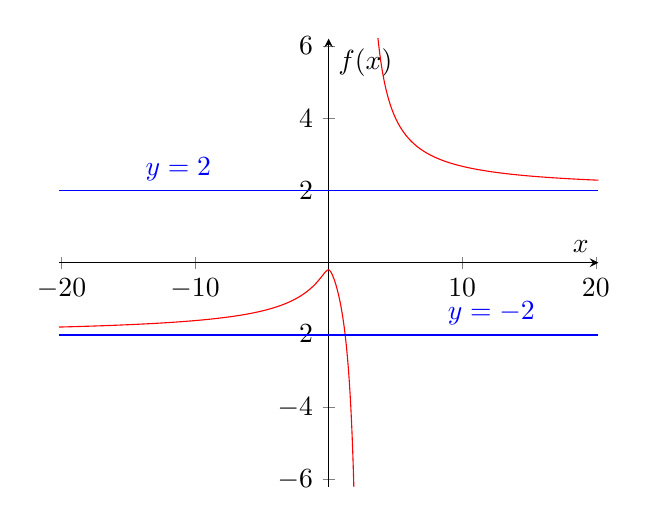
\begin{tikzpicture}
\begin{axis}[ axis x line=middle, axis y line=middle,xmax=20.2,ymax=6.2,xmin=-20.2,ymin=-6.2,ylabel=$f(x)$, xlabel=$x$, legend pos = north west]
\addplot[domain= -20.2:2.4, color = red, samples = 1000]{(16*x^2+1)^0.5/(2*x - 5)};
\addplot[domain= 2.6:20.2, color = red, samples = 1000]{(16*x^2+1)^0.5/(2*x - 5)};
\addplot[domain= -20.2:20.2, color = blue]{2}
node[ pos = 0.3, above left] {$y = 2$};
\addplot[domain= -20.2:20.2, color = blue]{-2}
node[ pos = 0.9, above left] {$y = -2$};
    \end{axis}
\end{tikzpicture}
\end{center}

\[ f(x) = \frac{\sqrt{16x^2+1}}{2x - 5} \]
对于这个函数,x goes to $\infty$的Limit是:${\lim_{x \to \infty} f(x) = \underline{\hbox to 5mm{}}}$;从图像上来看,随着自变量$x$的增大,$f(x)$的图像越来越接近于横线$y = \underline{\hbox to 5mm{}}$(整数/不存在)。

x goes to -$\infty$的Limit是:${\lim_{x \to -\infty} f(x) = \underline{\hbox to 5mm{}}}$;从图像上来看,随着自变量$x$的减小,$f(x)$的图像越来越接近于横线$y = \underline{\hbox to 5mm{}}$(整数/不存在)。


\begin{center}
\begin{tikzpicture}
\begin{axis}[ axis x line=middle, axis y line=middle,xmax=10.2,ymax=4.2,xmin=-10.2,ymin=-4.2,ylabel=$f(x)$, xlabel=$x$, legend pos = north west,x=0.5cm,y=0.5cm]
\addplot[domain= -10.2:10.2, color = red, samples = 1000]{(x^2-1)/(x^2+1)};
\addplot[domain= -10.2:10.2, color = blue]{1}
node[ pos = 0.9, above left] {$y = 1$};
    \end{axis}
\end{tikzpicture}
\end{center}

\[ f(x) = \frac{x^2-1}{x^2+1} \]
对于这个函数,x goes to $\infty$的Limit是:${\lim_{x \to \infty} f(x) = \underline{\hbox to 5mm{}}}$;从图像上来看,随着自变量$x$的增大,$f(x)$的图像越来越接近于横线$y = \underline{\hbox to 5mm{}}$(整数/不存在)。

x goes to -$\infty$的Limit是:${\lim_{x \to -\infty} f(x) = \underline{\hbox to 5mm{}}}$;从图像上来看,随着自变量$x$的减小,$f(x)$的图像越来越接近于横线$y = \underline{\hbox to 5mm{}}$(整数/不存在)。


\begin{center}
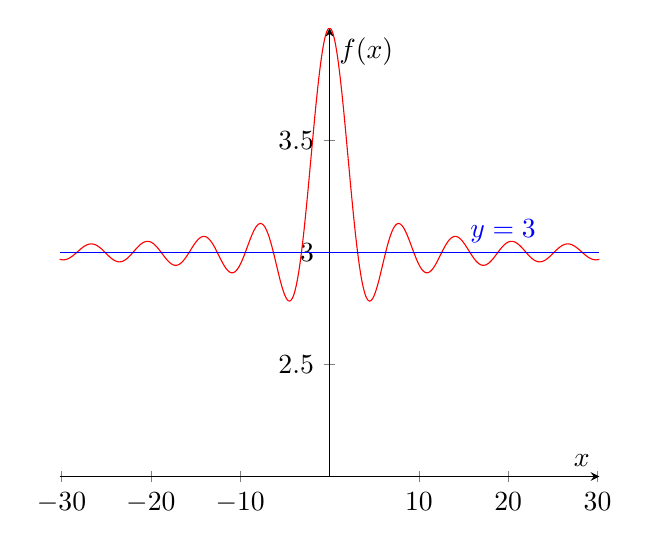
\begin{tikzpicture}
\begin{axis}[ axis x line=middle, axis y line=middle, ymin = 2, ylabel=$f(x)$, xlabel=$x$, legend pos = north west]
\addplot[domain= -30.2:30.2, color = red, samples = 1000]{(3*x+sin(deg(x)))/x};
\addplot[domain= -30.2:30.2, color = blue]{3}
node[ pos = 0.9, above left] {$y = 3$};
    \end{axis}
\end{tikzpicture}
\end{center}

\[ f(x) = \frac{3x+\sin{x}}{x} \]
对于这个函数,x goes to $\infty$的Limit是:${\lim_{x \to \infty} f(x) = \underline{\hbox to 5mm{}}}$;从图像上来看,随着自变量$x$的增大,$f(x)$的图像越来越接近于横线$y = \underline{\hbox to 5mm{}}$(整数/不存在)。

x goes to -$\infty$的Limit是:${\lim_{x \to -\infty} f(x) = \underline{\hbox to 5mm{}}}$;从图像上来看,随着自变量$x$的减小,$f(x)$的图像越来越接近于横线$y = \underline{\hbox to 5mm{}}$(整数/不存在)。

随着$x$趋近于$\infty$或$x$趋近于$-\infty$,函数$f(x)$的Limits是L,即:
\[ {\lim_{x \to \infty} f(x) = L} \qquad  \text{or} \qquad {\lim_{x \to -\infty} f(x) = L}\]
则函数图像在$x$ goes to $\infty$或在$x$ goes to $-\infty$时,图像一定不断\underline{\hbox to 5mm{}}(靠近/远离)$y = \underline{\hbox to 5mm{}}$这条直线,所以我们把$y=\underline{\hbox to 5mm{}}$称为$f(x)$的Horizontal Asymptote(水平渐近线)。

\paragraph{总结}
The Line $y=L$ is called a \textcolor{red}{horizontal asymptote} of the graph of function $f(x)$ if either
\[ {\lim_{x \to \infty} f(x) = L} \qquad  \text{or} \qquad {\lim_{x \to -\infty} f(x) = L}\]

\paragraph{发现}
Horizontal Asymptote可能有几条?

1. $f(x) = x^2$

 x goes to $\infty$的Limit是:${\lim_{x \to \infty} f(x) = \underline{\hbox to 5mm{}}}$;意思是随着自变量$x$的增大,$f(x)$的图像越来越接近于横线$y = \underline{\hbox to 5mm{}}$(整数/不存在)。

x goes to -$\infty$的Limit是:${\lim_{x \to -\infty} f(x) = \underline{\hbox to 5mm{}}}$;意思是随着自变量$x$的减小,$f(x)$的图像越来越接近于横线$y = \underline{\hbox to 5mm{}}$(整数/不存在)。

综上所述,$x$在趋近于无穷大时的Horizontal Asymptote为横线$y = \underline{\hbox to 5mm{}}(整数/不存在)$,在趋近于无穷小时的Horizontal Asymptote为横线$y = \underline{\hbox to 5mm{}}$(整数/不存在),共\underline{\hbox to 5mm{}}(整数)条。

2. $f(x) = e^x$

 x goes to $\infty$的Limit是:${\lim_{x \to \infty} f(x) = \underline{\hbox to 5mm{}}}$;意思是随着自变量$x$的增大,$f(x)$的图像越来越接近于横线$y = \underline{\hbox to 5mm{}}$(整数/不存在)。

x goes to -$\infty$的Limit是:${\lim_{x \to -\infty} f(x) = \underline{\hbox to 5mm{}}}$;意思是随着自变量$x$的减小,$f(x)$的图像越来越接近于横线$y = \underline{\hbox to 5mm{}}$(整数/不存在)。

综上所述,$x$在趋近于无穷大时的Horizontal Asymptote为横线$y = \underline{\hbox to 5mm{}}(整数/不存在)$,在趋近于无穷小时的Horizontal Asymptote为横线$y = \underline{\hbox to 5mm{}}$(整数/不存在),共\underline{\hbox to 5mm{}}(整数)条。

3. $f(x) = \frac{8x^2+5x-3}{4x^2+1}$

 x goes to $\infty$的Limit是:${\lim_{x \to \infty} f(x) = \underline{\hbox to 5mm{}}}$;意思是随着自变量$x$的增大,$f(x)$的图像越来越接近于横线$y = \underline{\hbox to 5mm{}}$(整数/不存在)。

x goes to -$\infty$的Limit是:${\lim_{x \to -\infty} f(x) = \underline{\hbox to 5mm{}}}$;意思是随着自变量$x$的减小,$f(x)$的图像越来越接近于横线$y = \underline{\hbox to 5mm{}}$(整数/不存在)。

综上所述,$x$在趋近于无穷大时的Horizontal Asymptote为横线$y = \underline{\hbox to 5mm{}}(整数/不存在)$,在趋近于无穷小时的Horizontal Asymptote为横线$y = \underline{\hbox to 5mm{}}$(整数/不存在),共\underline{\hbox to 5mm{}}(整数)条。


4. $f(x) = \frac{\sqrt{x^2-3}}{x-5}$

 x goes to $\infty$的Limit是:${\lim_{x \to \infty} f(x) = \underline{\hbox to 5mm{}}}$;意思是随着自变量$x$的增大,$f(x)$的图像越来越接近于横线$y = \underline{\hbox to 5mm{}}$(整数/不存在)。

x goes to -$\infty$的Limit是:${\lim_{x \to -\infty} f(x) = \underline{\hbox to 5mm{}}}$;意思是随着自变量$x$的减小,$f(x)$的图像越来越接近于横线$y = \underline{\hbox to 5mm{}}$(整数/不存在)。

综上所述,$x$在趋近于无穷大时的Horizontal Asymptote为横线$y = \underline{\hbox to 5mm{}}(整数/不存在)$,在趋近于无穷小时的Horizontal Asymptote为横线$y = \underline{\hbox to 5mm{}}$(整数/不存在),共\underline{\hbox to 5mm{}}(整数)条。

\paragraph{总结}
由于$x$趋近于$\infty$与$x$趋近于$-\infty$时的limit只可能有 \underline{\hbox to 5mm{}}种不同情况,所以函数的Horizontal Asymptotes最多只可能有 \underline{\hbox to 5mm{}}条。

\paragraph{游戏}
对以下函数,分别求${\lim_{x \to \infty}}$以及${\lim_{x \to -\infty}}$,并指出函数有几条Horizontal Asymptote,以及Horizontal Asymptote的方程。

(主线任务)
\[f(x) = \sqrt{x^2+x} - \sqrt{x^2-x}\]
\[{\lim_{x \to \infty} f(x) = \underline{\hbox to 5mm{}}}\]
\[{\lim_{x \to -\infty} f(x) = \underline{\hbox to 5mm{}}}\]
函数有\underline{\hbox to 5mm{}}条Horizontal Asymptote。
第一条的方程是\underline{\hbox to 5mm{}}(x=/y=/不存在);第二条的方程是\underline{\hbox to 5mm{}}(x=/y=/不存在)。

\[f(x) = \frac{ax^2+12}{x^2+b}\]
\[{\lim_{x \to \infty} f(x) = \underline{\hbox to 5mm{}}}\]
\[{\lim_{x \to -\infty} f(x) = \underline{\hbox to 5mm{}}}\]
函数有\underline{\hbox to 5mm{}}条Horizontal Asymptote。
第一条的方程是\underline{\hbox to 5mm{}}(x=/y=/不存在);第二条的方程是\underline{\hbox to 5mm{}}(x=/y=/不存在)。

(支线任务)
\[f(x) = \frac{3x^2+1}{2x^2+x+1}\]
\[{\lim_{x \to \infty} f(x) = \underline{\hbox to 5mm{}}}\]
\[{\lim_{x \to -\infty} f(x) = \underline{\hbox to 5mm{}}}\]
函数有\underline{\hbox to 5mm{}}条Horizontal Asymptote。
第一条的方程是\underline{\hbox to 5mm{}}(x=/y=/不存在);第二条的方程是\underline{\hbox to 5mm{}}(x=/y=/不存在)。

\[f(x) = \sqrt{x^2+ax} - \sqrt{x^2+bx}\]
\[{\lim_{x \to \infty} f(x) = \underline{\hbox to 5mm{}}}\]
\[{\lim_{x \to -\infty} f(x) = \underline{\hbox to 5mm{}}}\]
函数有\underline{\hbox to 5mm{}}条Horizontal Asymptote。
第一条的方程是\underline{\hbox to 5mm{}}(x=/y=/不存在);第二条的方程是\underline{\hbox to 5mm{}}(x=/y=/不存在)。

\[f(x) = \frac{\sqrt{2x^2+1}}{3x-5}\]
\[{\lim_{x \to \infty} f(x) = \underline{\hbox to 5mm{}}}\]
\[{\lim_{x \to -\infty} f(x) = \underline{\hbox to 5mm{}}}\]
函数有\underline{\hbox to 5mm{}}条Horizontal Asymptote。
第一条的方程是\underline{\hbox to 5mm{}}(x=/y=/不存在);第二条的方程是\underline{\hbox to 5mm{}}(x=/y=/不存在)。

\[f(x) = \frac{1+x^4}{x^2-x^4}\]
\[{\lim_{x \to \infty} f(x) = \underline{\hbox to 5mm{}}}\]
\[{\lim_{x \to -\infty} f(x) = \underline{\hbox to 5mm{}}}\]
函数有\underline{\hbox to 5mm{}}条Horizontal Asymptote。
第一条的方程是\underline{\hbox to 5mm{}}(x=/y=/不存在);第二条的方程是\underline{\hbox to 5mm{}}(x=/y=/不存在)。

\[f(x) = \frac{5\sqrt{x}}{\sqrt{x}-1}\]
\[{\lim_{x \to \infty} f(x) = \underline{\hbox to 5mm{}}}\]
\[{\lim_{x \to -\infty} f(x) = \underline{\hbox to 5mm{}}}\]
函数有\underline{\hbox to 5mm{}}条Horizontal Asymptote。
第一条的方程是\underline{\hbox to 5mm{}}(x=/y=/不存在);第二条的方程是\underline{\hbox to 5mm{}}(x=/y=/不存在)。

\[f(x) = \frac{2x+1}{x-2}\]
\[{\lim_{x \to \infty} f(x) = \underline{\hbox to 5mm{}}}\]
\[{\lim_{x \to -\infty} f(x) = \underline{\hbox to 5mm{}}}\]
函数有\underline{\hbox to 5mm{}}条Horizontal Asymptote。
第一条的方程是\underline{\hbox to 5mm{}}(x=/y=/不存在);第二条的方程是\underline{\hbox to 5mm{}}(x=/y=/不存在)。

\paragraph{注意}

\begin{center}
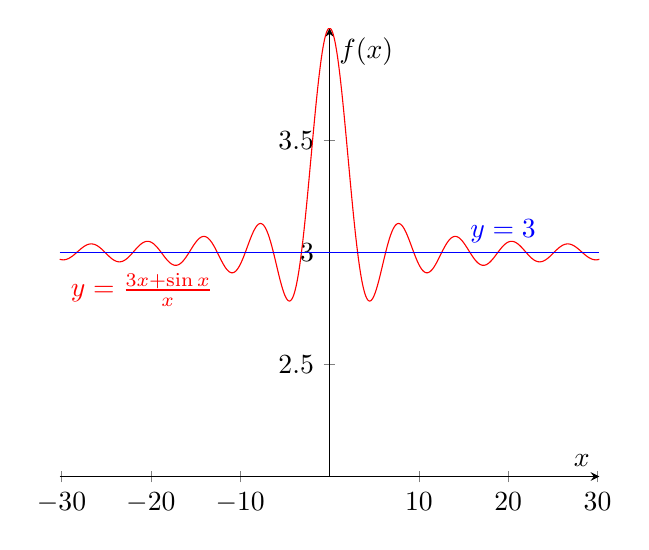
\begin{tikzpicture}
\begin{axis}[ axis x line=middle, axis y line=middle, ymin = 2, ylabel=$f(x)$, xlabel=$x$, legend pos = north west]
\addplot[domain= -30.2:30.2, color = red, samples = 1000]{(3*x+sin(deg(x)))/x}
node[ pos = 0.3, below left] {$y = \frac{3x+\sin{x}}{x}$};
\addplot[domain= -30.2:30.2, color = blue]{3}
node[ pos = 0.9, above left] {$y = 3$};
    \end{axis}
\end{tikzpicture}
\end{center}

可以看出,函数$f(x) = \frac{3x+\sin{x}}{x}$ 的 horizontal Asymptote是\underline{\hbox to 5mm{}}(x=/y=/不存在),函数的图像和它的horizontal asymptote有\underline{\hbox to 5mm{}}(整数/$\infty$)个交点。

这说明,函数的图像和它的horizontal asymptote\underline{\hbox to 5mm{}}(可以/不能)相交。

\subsection{Advanced Techniques of Calculating Limits}
\subsubsection{The Sandwich Theorem}
\paragraph{探索}
之前我们介绍了一些常规的Limit求法,下面我们来升级一下我们的操作,介绍一些更狂霸拽酷炫的求法。首先我们需要定义的是函数的比大小问题。

假设我们有三个函数:$f(x)$,$g(x)$,$h(x)$,那么我们如何能够判断三个函数的大小呢?注意大多数函数是不能够比大小的,例如:

\begin{center}
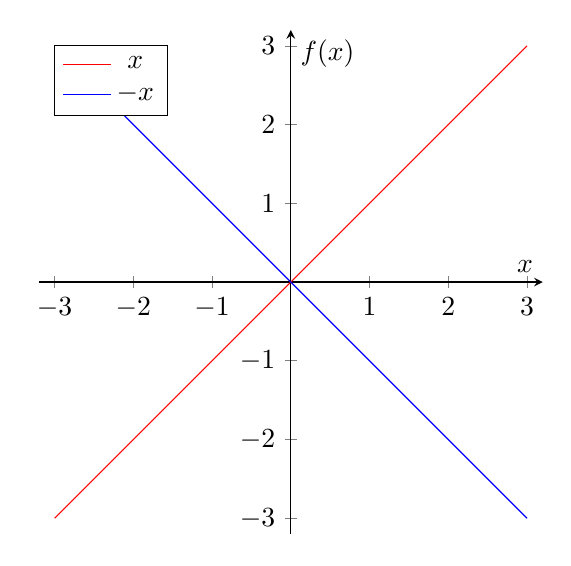
\begin{tikzpicture}
\begin{axis}[ axis x line=middle, axis y line=middle,xmax=3.2,ymax=3.2,xmin=-3.2,ymin=-3.2,ylabel=$f(x)$, xlabel=$x$, legend pos = north west,x=1cm,y=1cm]
\addplot[domain= -3:3, color = red]{x};
\addlegendentry{$x$}
\addplot[domain= -3:3, color = blue]{-x};
\addlegendentry{$-x$}
    \end{axis}
\end{tikzpicture}
\end{center}

\[f(x) = x; g(x) = -x\]

这就非常尴尬了,在$x<0$的范围内,好像$f(x)$一直比$g(x)$\underline{\hbox to 5mm{}}(小/大),而在$x>0$的范围内,$f(x)$比$g(x)$\underline{\hbox to 5mm{}}(小/大),所以我们说,$f(x)$和$g(x)$在他们的domain上是\underline{\hbox to 5mm{}}(incomparable/comparable)的。

下面这两个函数就非常友好了,我们可以一下就说出两个函数的大小关系:

\begin{center}
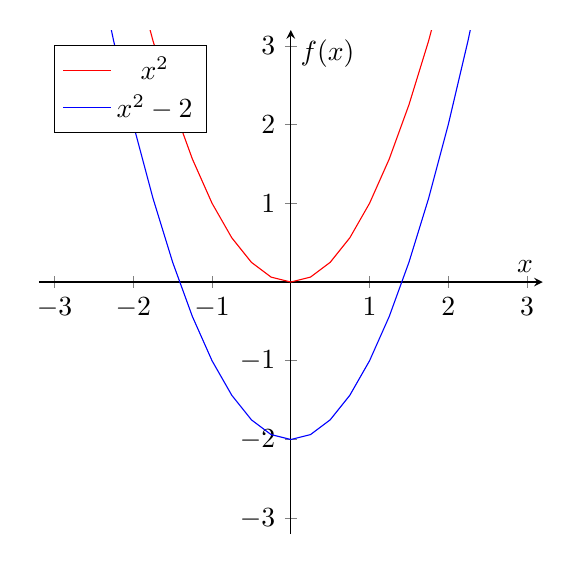
\begin{tikzpicture}
\begin{axis}[ axis x line=middle, axis y line=middle,xmax=3.2,ymax=3.2,xmin=-3.2,ymin=-3.2,ylabel=$f(x)$, xlabel=$x$, legend pos = north west,x=1cm,y=1cm]
\addplot[domain= -3:3, color = red]{x^2};
\addlegendentry{$x^2$}
\addplot[domain= -3:3, color = blue]{x^2-2};
\addlegendentry{$x^2-2$}
    \end{axis}
\end{tikzpicture}
\end{center}

\[f(x) = x^2; g(x) = x^2-2\]
在整个$f(x)$和$g(x)$的domain中,$f(x)$的值一直都\underline{\hbox to 5mm{}}(大于/小于)$g(x)$的值,所以我们可以说:$f(x)\underline{\hbox to 5mm{}}(>/</=) g(x)$。

从图像上来说,如果$f(x)<g(x)$,那么$f(x)$的图像永远在$g(x)$的\underline{\hbox to 5mm{}}(上方/下方),$f(x)$与$g(x)$的图像\underline{\hbox to 5mm{}}(有交点/无交点);如果$f(x)>g(x)$,那么$f(x)$的图像永远在$g(x)$的\underline{\hbox to 5mm{}}(上方/下方),$f(x)$与$g(x)$的图像\underline{\hbox to 5mm{}}(有可能有/一定没有)交点;如果两个函数是incomparable的,那么他们(有可能有/一定没有)交点。

如果$g(x) < f(x) < h(x)$,则$f(x)$的图像一定在\underline{\hbox to 5mm{}}($g(x)/h(x)$)的上方,并且一定在\underline{\hbox to 5mm{}}($g(x)/h(x)$)的下方。

换句话说,$f(x)$的图像一定在$h(x)$与$g(x)$\underline{\hbox to 5mm{}}

\begin{center}
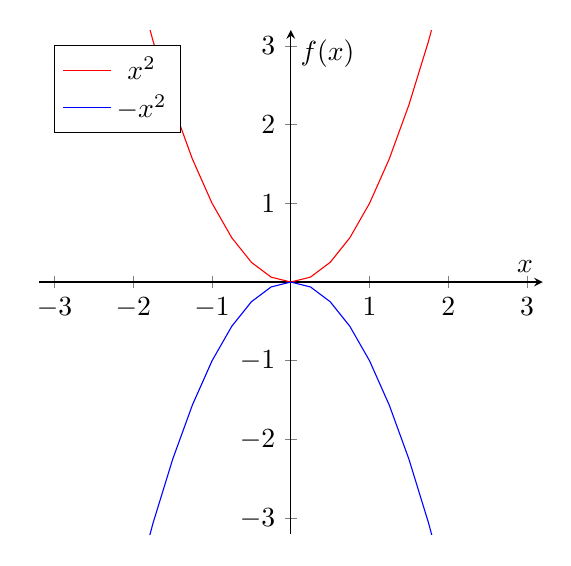
\begin{tikzpicture}
\begin{axis}[ axis x line=middle, axis y line=middle,xmax=3.2,ymax=3.2,xmin=-3.2,ymin=-3.2,ylabel=$f(x)$, xlabel=$x$, legend pos = north west,x=1cm,y=1cm]
\addplot[domain= -3:3, color = red]{x^2};
\addlegendentry{$x^2$}
\addplot[domain= -3:3, color = blue]{-x^2};
\addlegendentry{$-x^2$}
    \end{axis}
\end{tikzpicture}
\end{center}

在整个$f(x)$和$g(x)$的domain中,$f(x)$的值一直都\underline{\hbox to 5mm{}}(不大于/不小于)$g(x)$的值,所以我们可以说:$f(x)\underline{\hbox to 5mm{}}(>/</\geq/\leq/=) g(x)$。这个情况和上一种情况的区别是,$f(x)$\underline{\hbox to 5mm{}}(必须/不必)一直大于$g(x)$,可以有(小于/等于/小于或等于)$g(x)$的点,$f(x)$与$g(x)$的图像\underline{\hbox to 5mm{}}(有可能有/一定没有)交点。

\paragraph{游戏}
判断以下函数的大小关系,在填空中填写$>,<,\geq,\leq$ 或 Incomparable,use graphing calculator if necessary.
\[f(x) = x^2\underline{\hbox to 5mm{}} g(x) =  x    \qquad   f(x) = x+10  \underline{\hbox to 5mm{}} g(x) = -x^2-10\]
\[f(x) =\cos{x}-2\underline{\hbox to 5mm{}} g(x) = \sin{x+2}    \qquad   f(x) = 2^x  \underline{\hbox to 5mm{}} g(x) = e^x\]
\[f(x) =\sin{x} \underline{\hbox to 5mm{}} g(x) = x\cdot \sin{x}    \qquad   f(x) = \frac{1}{x} \underline{\hbox to 5mm{}} g(x) = -\frac{1}{x}\]

\paragraph{发现}

我们来观察一下下面这几个函数:
\begin{center}
     \begin{tikzpicture}
        \begin{axis}[
            xmin=-10,xmax=10,
            xlabel={z},
            ymin=-10,ymax=10,
        xlabel={$x$},  
        ylabel={$y$},
        axis lines=middle] 
    \addplot+[red,thick,domain=-5:5,no marks] {\x^2+3} node[above] {$h(x)$};
    \addplot+[red,thick,domain=-5:5,no marks] {-\x^2-3} node[above] {$g(x)$};;
    \end{axis}
  %Hobby package  
    \draw (0 ,4) to [out angle = 0, in angle = 180, curve through ={(1.5,1.5)  . . (2,2) ..(4,2.1)  }] (6,6) node[above] {$f(x)$};% curve 
\end{tikzpicture}
\end{center}
两个红色的函数分别是$g(x) = -x^2 - 3$、$h(x) = x^2+3$ ,从图像上可以看出来,黑色的函数$f(x)$被“夹”在$g(x)$和$h(x)$之间,数学上可以表示为$g(x)\underline{\hbox to 5mm{}}f(x)\underline{\hbox to 5mm{}}h(x)$

根据之前学过的知识,我们知道:

\[{\lim_{x \to 0} g(x)} = \underline{\hbox to 5mm{}} \qquad {\lim_{x \to 0} h(x)} = \underline{\hbox to 5mm{}} \]

由于$f(x)$是连续的,所以我们知道:

\[{\lim_{x \to 0} f(x)} = f(\underline{\hbox to 5mm{}})\]

这也是$f(x)$图像和y轴的\underline{\hbox to 5mm{}}

此时我们观察图像,由于\[{\lim_{x \to 0} g(x)} = g(\underline{\hbox to 5mm{}}), {\lim_{x \to 0} f(x)} = f(\underline{\hbox to 5mm{}}), {\lim_{x \to 0} h(x)} = h(\underline{\hbox to 5mm{}}) \]
又因为$g(x)\underline{\hbox to 5mm{}}f(x)\underline{\hbox to 5mm{}}h(x)$,所以不管a是任何值,$g(a)\underline{\hbox to 5mm{}}f(a)\underline{\hbox to 5mm{}}h(a)$。
我们可以知道:\[{\lim_{x \to 0} g(x)} \underline{\hbox to 5mm{}}(>/</=){\lim_{x \to 0} f(x)} \underline{\hbox to 5mm{}}(>/</=){\lim_{x \to 0} h(x)} \]
在这道题上,也就是\[\underline{\hbox to 5mm{}}(>/</=)(\text{数字})<{\lim_{x \to 0} f(x)} <\underline{\hbox to 5mm{}}(>/</=)(\text{数字}) \]

下面我们把上面的函数往下“压”,上面的函数往上“推”,分别变成$h(x) = x^2+1$以及$g(x) = -x^2-1$,此时如果再定义一个函数$f(x)$满足$g(x)<f(x)<h(x)$的话,图像大致是这个样子:
\begin{center}
     \begin{tikzpicture}
        \begin{axis}[
            xmin=-5,xmax=5,
            xlabel={z},
            ymin=-5,ymax=5,
        xlabel={$x$},  
        ylabel={$y$},
        axis lines=middle] 
    \addplot+[red,thick,domain=-5:5,no marks] {\x^2+1} node[above] {$h(x)$};
    \addplot+[red,thick,domain=-5:5,no marks] {-\x^2-1} node[above] {$g(x)$};;
    \end{axis}
  %Hobby package  
    \draw (0 ,4) to [out angle = 0, in angle = 150, curve through ={(1,3)  . . (2,2) ..(3,2.3)  }] (6,4) node[above] {$f(x)$};% curve 
\end{tikzpicture}
\end{center}

和上一题一样,因为$f(x), g(x), h(x)$的大小关系没有发生改变,所以:
\[{\lim_{x \to 0} g(x)} \underline{\hbox to 5mm{}}(>/</=){\lim_{x \to 0} f(x)} \underline{\hbox to 5mm{}}(>/</=){\lim_{x \to 0} h(x)} \]
在这道题上,也就是\[\underline{\hbox to 5mm{}}(>/</=)(\text{数字})<{\lim_{x \to 0} f(x)} <\underline{\hbox to 5mm{}}(>/</=)(\text{数字}) \]

如果我们继续在保证$f(x)$与$g(x)$不是incomparable的情况下,把上面的函数继续往下“压”,上面的函数往上“推”。最终,我们将得到这样的两个函数:

\begin{center}
     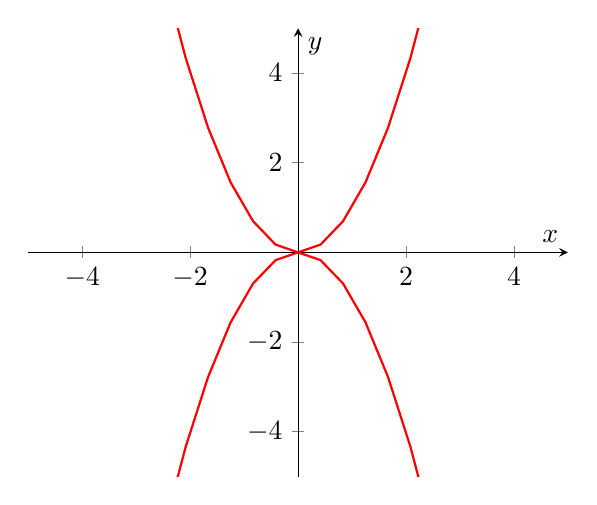
\begin{tikzpicture}
        \begin{axis}[
            xmin=-5,xmax=5,
            xlabel={z},
            ymin=-5,ymax=5,
        xlabel={$x$},  
        ylabel={$y$},
        axis lines=middle] 
    \addplot+[red,thick,domain=-5:5,no marks] {\x^2} node[above] {$h(x)$};
    \addplot+[red,thick,domain=-5:5,no marks] {-\x^2} node[above] {$g(x)$};
    \end{axis}
\end{tikzpicture}
\end{center}

\[h(x) = x^2 \qquad g(x) = - x^2\]

这下就有意思了。如果此时$f(x)$依然满足$g(x)\leq f(x)\leq h(x)$,也就是说$f(x)$依然活在$h(x)$和$g(x)$之间的话,它的图像只能长成什么样呢?(请自行脑补图像,然后向下看)

\begin{center}
     \begin{tikzpicture}
        \begin{axis}[
            xmin=-5,xmax=5,
            xlabel={z},
            ymin=-5,ymax=5,
        xlabel={$x$},  
        ylabel={$y$},
        axis lines=middle] 
    \addplot+[red,thick,domain=-5:5,no marks] {\x^2} node[above] {$h(x)$};
    \addplot+[red,thick,domain=-5:5,no marks] {-\x^2} node[above] {$g(x)$};
    \end{axis}
    \draw (0,3) to [ curve through ={(3,3)..(3.4,2.83)..(4,2.8) }] (6,4) node[above] {$f(x)$};
\end{tikzpicture}
\end{center}

和上一题一样,因为$f(x), g(x), h(x)$的大小关系没有发生改变,所以:
\[{\lim_{x \to 0} g(x)} \underline{\hbox to 5mm{}}(>/\geq/</\leq/=){\lim_{x \to 0} f(x)} \underline{\hbox to 5mm{}}(>/\geq/</\leq/=){\lim_{x \to 0} h(x)} \]
然而因为${\lim_{x \to 0} g(x)}$和${\lim_{x \to 0} h(x)}$在$x=0$处的Limit是\underline{\hbox to 5mm{}}(相等/不等)的,这个式子也就直接变成了:
\[{\lim_{x \to 0} g(x)} \underline{\hbox to 5mm{}}(>/\geq/</\leq/=){\lim_{x \to 0} f(x)} \underline{\hbox to 5mm{}}(>/\geq/</\leq/=){\lim_{x \to 0} h(x)} \]

在这道题上,也就是\[\underline{\hbox to 5mm{}}\text{(数字)}\leq{\lim_{x \to 0} f(x)} <\underline{\hbox to 5mm{}} \leq \text{数字}) \],或者可以直接写作:
\[{\lim_{x \to 0} f(x)} =  \underline{\hbox to 5mm{}}\text{(数字)}\]

两个函数,$h(x)$从上往下“挤”,$g(x)$从下往上“挤”,两个函数在$x=0$处“粘在一起”,终于把$f(x)$牢牢地“夹”在了两个函数中间,使得$f(x)$的Limit别无选择,只能和$g(x)$与$h(x)$在该点的Limit相等,用这种方法求$f(x)$在某一点的Limit。所以我们管这个定理叫做“Squeeze Theorem”(夹逼定理)或“Sandwich Theorem”(三明治定理)。

通俗一点说,我们可以管$h(x)$叫做“上皮”,$g(x)$叫做“下皮”,$f(x)$叫做“馅”;一定要记住,在Squeeze Theorem的过程中,首先确保下皮$<$馅$<$上皮。

下面来观察这三个函数:
\begin{center}
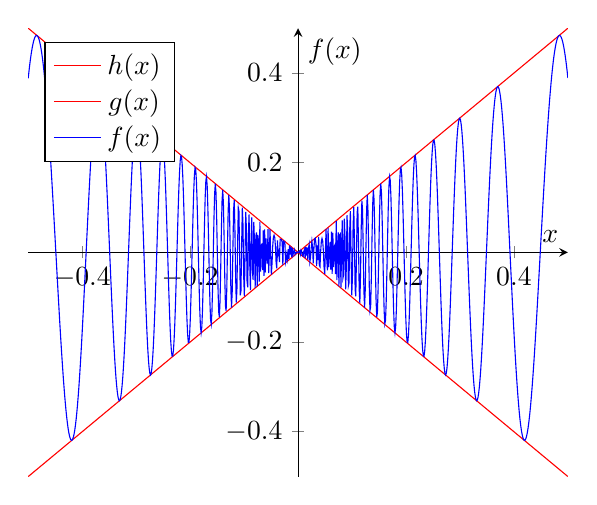
\begin{tikzpicture}
\begin{axis}[ axis x line=middle, axis y line=middle,xmax=0.5,ymax=0.5,xmin=-0.5,ymin=-0.5,ylabel=$f(x)$, xlabel=$x$, legend pos = north west]
\addplot[domain= -0.5:0.5, color = red]{x};
\addlegendentry{$h(x)$}
\addplot[domain= -0.5:0.5, color = red]{-x};
\addlegendentry{$g(x)$}
\addplot[domain=-0.5:0.5, color = blue, samples = 800] {x * sin(180/(x/pi))};
\addlegendentry{$f(x)$}
    \end{axis}
\end{tikzpicture}
\end{center}
\[f(x) = x \sin{\frac{1}{x}}   \qquad  g(x) = -x \qquad h(x)=x\]
\[{\lim_{x \to 0} x\sin{\frac{1}{x}}} = ?\]
如果我们尝试通过Limit Law来求的话,会遇到这样的问题:
\[{\lim_{x \to 0} x\sin{\frac{1}{x}}} = {\lim_{x \to 0} x} * {\lim_{x \to 0} \sin{\frac{1}{x}}} = 0* ???\]
记性好的话你应该记得,${\lim_{x \to 0} \sin{\frac{1}{x}}}$是Limit does not exist的【链接:Limit does not exist】。这可怎么办?还好有三明治(定理)。

在$x>0$时,三明治的“上皮”是\underline{\hbox to 5mm{}},三明治的下皮是\underline{\hbox to 5mm{}},三明治的馅是\underline{\hbox to 5mm{}}。因为我们只观察了函数在$x>0$时的状况来推知$x=0$的Limit,所以我们通过Squeeze Theorem能得到函数的\underline{\hbox to 5mm{}}(right hand limit/left hand limit/ limit)。

在$x>0$时三个函数的大小关系满足$g(x) \underline{\hbox to 5mm{}} f(x) \underline{\hbox to 5mm{}} h(x)$,被“squeeze”而使得上下皮和馅“粘在一起”的点是$x=\underline{\hbox to 5mm{}}$处。所以必须有:

\[{\lim_{x \to 0^+} g(x)} = {\lim_{x \to 0^+} h(x)} = \underline{\hbox to 5mm{}}\]

\[\underline{\hbox to 5mm{}}\text{(数字)} \leq {\lim_{x \to 0^+} f(x)} \leq \underline{\hbox to 5mm{}}\text{(数字)}\]
所以${\lim_{x \to 0^+} f(x)} = \underline{\hbox to 5mm{}}$

在$x<0$时,三明治的“上皮”是\underline{\hbox to 5mm{}},三明治的下皮是\underline{\hbox to 5mm{}},三明治的馅是\underline{\hbox to 5mm{}}。因为我们只观察了函数在$x<0$时的状况来推知$x=0$的Limit,所以我们通过Squeeze Theorem能得到函数的\underline{\hbox to 5mm{}}(right hand limit/left hand limit/ limit)。

在$x<0$时三个函数的大小关系满足$g(x) \underline{\hbox to 5mm{}} f(x) \underline{\hbox to 5mm{}} h(x)$,被“squeeze”而使得上下皮和馅“粘在一起”的点是$x=\underline{\hbox to 5mm{}}$处。所以必须有:

\[{\lim_{x \to 0^-} g(x)} = {\lim_{x \to 0^-} h(x)} = \underline{\hbox to 5mm{}}\]
\[\underline{\hbox to 5mm{}}\text{(数字)} \leq {\lim_{x \to 0^-} f(x)} \leq \underline{\hbox to 5mm{}}\text{(数字)}\]
所以${\lim_{x \to 0^-} f(x)} = \underline{\hbox to 5mm{}}$

于是我们知道${\lim_{x \to 0+} f(x)} \underline{\hbox to 5mm{}} {\lim_{x \to 0-} f(x)} = \underline{\hbox to 5mm{}}$

已知当$-1\leq x \leq 1$时,\[\sqrt{5-2x^2} \leq f(x) \leq \sqrt{5-x^2}\],${\lim_{x \to 0} f(x) = ?}$

在$-1\leq x \leq 1$时,三明治的“上皮”是\underline{\hbox to 5mm{}},三明治的下皮是\underline{\hbox to 5mm{}},三明治的馅是\underline{\hbox to 5mm{}},因为我们同时观察了$x<0$与$x>0$的情况推知$x=0$的Limit,所以我们通过Squeeze Theorem能得到函数的\underline{\hbox to 5mm{}}(right hand limit/left hand limit/ limit)。

在$-1\leq x \leq 1$时三个函数的大小关系满足$g(x) \underline{\hbox to 5mm{}} f(x) \underline{\hbox to 5mm{}} h(x)$,被“squeeze”而使得上下皮和馅“粘在一起”的点是$x=\underline{\hbox to 5mm{}}$处。所以必须有:

\[{\lim_{x \to 0} g(x)} = {\lim_{x \to 0} h(x)} = \underline{\hbox to 5mm{}}\]

\[\underline{\hbox to 5mm{}}\text{(数字)} \leq {\lim_{x \to 0} f(x)} \leq \underline{\hbox to 5mm{}}\text{(数字)}\]
所以${\lim_{x \to 0} f(x)} = \underline{\hbox to 5mm{}}$

\paragraph{总结}

总的来说,使用squeeze theorem需要以下几个关键条件:

1. 已知三个函数$f(x)$、$h(x)$、$g(x)$。

2. 三个函数在某个区间上$a \leq x \leq b$,满足$g(x) \leq f(x) \leq h(x)$

3. 在该区间内的某个点$a \leq x_0 \leq b$,$g(x)$和$h(x)$“粘在一起了”,即:$g(x_0) = h(x_0)$,或者更严谨一些,应该是${\lim_{x \to x_0} g(x)} = {\lim_{x \to x_0} h(x)} = L $

此时我们就能够得到结论:${\lim_{x \to x_0} f(x)} = L$

If $g(x) \leq f(x) \leq g(x)$, when x is near a , and
\[{\lim_{x \to a} g(x)} = {\lim_{x \to a} h(x)} = L \],then \[{\lim_{x \to a} f(x)} = L\]

\paragraph{游戏}

1. 已知对于所有$x$,都有:\[3-x^2 \leq f(x) \leq 3\cos{x}\],求\[{\lim_{x \to 0} f(x)}\]

三明治的上皮是 \underline{\hbox to 5mm{}}。

三明治的下皮是 \underline{\hbox to 5mm{}}。

三明治的馅是 \underline{\hbox to 5mm{}}。

上下皮和馅的粘合部位是 \underline{\hbox to 5mm{}}(在该点,上皮=下皮)。

该点是否在上皮$>$下皮的区间内? \underline{\hbox to 5mm{}}(Y/N)。

\[{\lim_{x \to 0} f(x)} = \underline{\hbox to 5mm{}}\]

2. 已知对于所有0周围的点,都有:\[1-\frac{x^2}{6} < \frac{x\sin{x}}{2-2\cos{x}}<1\],求\[{\lim_{x \to 0} \frac{x\sin{x}}{2-2\cos{x}}}\]

三明治的上皮是 \underline{\hbox to 5mm{}}。

三明治的下皮是 \underline{\hbox to 5mm{}}。

三明治的馅是 \underline{\hbox to 5mm{}}。

上下皮和馅的粘合部位是 \underline{\hbox to 5mm{}}(在该点,上皮=下皮)。

该点是否在上皮$>$下皮的区间内? \underline{\hbox to 5mm{}}(Y/N)。

\[{\lim_{x \to 0} f(x)} = \underline{\hbox to 5mm{}}\]

3. 已知对于所有0周围的点,都有:\[\frac{1}{2}-\frac{x^2}{24} < \frac{1-\cos{x}}{x^2}<\frac{1}{2}\],求\[{\lim_{x \to 0} \frac{1-\cos{x}}{x^2}}\]

三明治的上皮是 \underline{\hbox to 5mm{}}。

三明治的下皮是 \underline{\hbox to 5mm{}}。

三明治的馅是 \underline{\hbox to 5mm{}}。

上下皮和馅的粘合部位是 \underline{\hbox to 5mm{}}(在该点,上皮=下皮)。

该点是否在上皮$>$下皮的区间内? \underline{\hbox to 5mm{}}(Y/N)。

\[{\lim_{x \to 0} f(x)} = \underline{\hbox to 5mm{}}\]

4. \[A(x) = x^2; B(x) = -x^2; C(x) = x^2\sin{\frac{1}{x}}\]
求\[{\lim_{x \to 0} x^2\sin{\frac{1}{x}}}\]

根据三角函数的特性,-1\underline{\hbox to 5mm{}}$\sin{x}$\underline{\hbox to 5mm{}}1,因x可以等于all real numbers,所以-1\underline{\hbox to 5mm{}}$\sin{1/x}$\underline{\hbox to 5mm{}}1 也成立。

故\[\underline{\hbox to 5mm{}}  \leq x^2*\sin{\frac{1}{x}} \leq \underline{\hbox to 5mm{}} \]

三明治的上皮是 \underline{\hbox to 5mm{}}。

三明治的下皮是 \underline{\hbox to 5mm{}}。

三明治的馅是 \underline{\hbox to 5mm{}}。

上下皮和馅的粘合部位是 \underline{\hbox to 5mm{}}(在该点,上皮=下皮)。

该点是否在上皮$>$下皮的区间内? \underline{\hbox to 5mm{}}(Y/N)。

\[{\lim_{x \to 0} x^2\sin{\frac{1}{x}}} = \underline{\hbox to 5mm{}}\]

\subsubsection{${\lim_{x \to 0} \frac{\sin{x}}{x}}$}
\paragraph{探索}

在求解一些特殊函数的limit时,我们可以发现,很多函数都是由一些基本的函数变化而来的,所以这些变化的“本源”函数就会非常关键。

在这里,我们先介绍第一个比较特殊的“本源”函数:
\[f(x) = \frac{\sin{x}}{x}\]
\begin{center}
\begin{tikzpicture}
\begin{axis}[ axis x line=middle, axis y line=middle,xmax=20.2,ymax=2.2,xmin=-20.2,ymin=-2.2,ylabel=$f(x)$, xlabel=$x$, legend pos = north west]
\addplot[domain= -20.2:20.2, color = red,samples = 1000]{sin(deg(x))/x};
\end{axis}
\end{tikzpicture}
\end{center}  

对于这个函数,使用无穷大的阶的理论【链接】不难看出:
\[ {\lim_{x \to \infty} \frac{\sin{x}}{x}} =  \underline{\hbox to 5mm{}}\]
\[ {\lim_{x \to -\infty} \frac{\sin{x}}{x}} =  \underline{\hbox to 5mm{}}\]
函数的Horizontal Asymptote 是$x = \underline{\hbox to 5mm{}}$

而\[\lim_{x \to 0} \frac{\sin{x}}{x}\] 则稍微复杂一些。首先,我们代入$x = 0$是不行的,因为函数的domain\underline{\hbox to 5mm{}}(包含/不包含)$x=0$。这个极限的运算过程有些费劲,目前你只需要掌握它的值就可以了:

\[{\lim_{x \to 0} \frac{\sin{x}}{x}} =  1\]

虽然暂时无法通过代数途径证明这个Limit,我们却可以从代数的角度来理解它:当x越接近于0时,$\sin{x}$与$x$的比值就越接近于\underline{\hbox to 5mm{}},这也就意味着当x的大小在0附近时,$\sin{x}$和$x$的值近似\underline{\hbox to 5mm{}}(相等/不等)。

我们可以把这两个函数的图像画出来:
\begin{center}
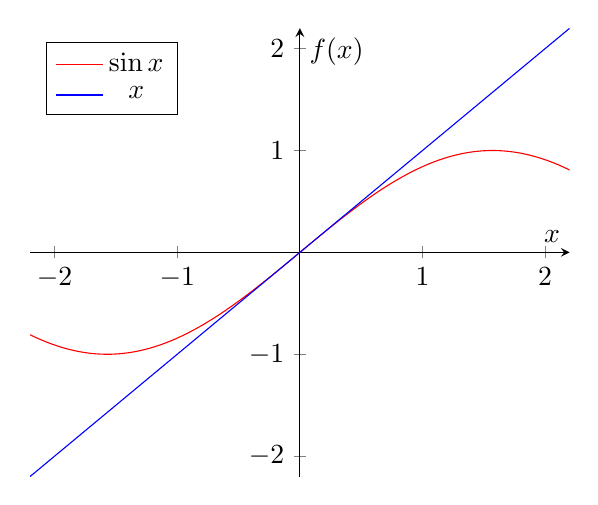
\begin{tikzpicture}
\begin{axis}[ axis x line=middle, axis y line=middle,xmax=2.2,ymax=2.2,xmin=-2.2,ymin=-2.2,ylabel=$f(x)$, xlabel=$x$, legend pos = north west]
\addplot[domain= -2.2:2.2, color = red,samples = 100]{sin(deg(x))};
\addlegendentry{$\sin{x}$};
\addplot[domain= -2.2:2.2, color = blue]{x};
\addlegendentry{$x$}
\end{axis}
\end{tikzpicture}
\end{center}  

可以看到,在$-0.5 \leq x \leq 0.5$这个区域,$\sin{x}$与$x$的图像几乎是\underline{\hbox to 5mm{}}(重合/分离)的。

\paragraph{发现}

了解了
\[{\lim_{x \to 0} \frac{\sin{x}}{x}} =  1\]
这个极限以后,我们在面对带有三角函数的$x \to 0$ 时的Limit时,就应该首先考虑它能不能换成形如$\frac{\sin{x}}{x}$的函数进行求解了。

\[\lim_{x \to 0} \frac{\sin{5x}}{x}\]

这个函数看上去和 $\frac{\sin{x}}{x}$长的有几分相似,我们可以给它做做“整容”,让它们变的更相似一些

\begin{eqnarray*}
{\lim_{x \to 0} \frac{\sin{5x}}{x}}\\
& = & {\lim_{x \to 0} \frac{\sin{5x}}{x} \cdot \frac{5}{5}}\\
& = & {\lim_{x \to 0} 5\cdot \frac{\sin{5x}}{x \cdot \underline{\hbox to 5mm{}}}}\\
& = & \underline{\hbox to 5mm{}} \cdot {\lim_{x \to 0} \frac{\sin{5x}}{\underline{\hbox to 5mm{}}}}
\end{eqnarray*}

这个时候我们就可以发现$x \to 0$ 和 $5x \to 0$本质其实是一样的,于是:
\begin{eqnarray*}
{\lim_{x \to 0} \frac{\sin{5x}}{5x}}\\
&= &{\lim_{5x \to 0} \frac{\sin{5x}}{5x}}\\
\text{设} u = 5x \\
&=& {\lim_{u \to 0} \frac{\sin{u}}{u}}\\
&=& \underline{\hbox to 5mm{}}
\end{eqnarray*}

所以
\[ \lim_{x \to 0} \frac{\sin{5x}}{x} = \underline{\hbox to 5mm{}} \cdot \lim_{x \to 0} \frac{\sin{5x}}{5x} = \underline{\hbox to 5mm{}} \cdot \underline{\hbox to 5mm{}} = \underline{\hbox to 5mm{}}\]

\begin{eqnarray*}
{\lim_{x \to 0} \frac{\sin{3x}}{4x}}\\
& = & {\lim_{x \to 0} \frac{\sin{3x}}{4x} \cdot \frac{3/4}{3/4}}\\
& = & \frac{3}{4} \cdot {\lim_{x \to 0} \frac{\sin{3x}}{\underline{\hbox to 5mm{}}}}\\
& = & \frac{3}{4} \cdot \underline{\hbox to 5mm{}}\\
& = & \underline{\hbox to 5mm{}}
\end{eqnarray*}

\begin{eqnarray*}
{\lim_{x \to 3} \frac{\sin{2x-6}}{x-3}}\\
& = & {\lim_{x \to 3} \frac{\sin{2x-6}}{x-3} \cdot \frac{2}{2}}\\
& = & \underline{\hbox to 5mm{}} \cdot {\lim_{x \to 3} \frac{\sin{2x-6}}{\underline{\hbox to 5mm{}}}}\\
\text{设} u = \underline{\hbox to 5mm{}} \\
& = & 2 \cdot {\lim_{u \to 0} \frac{\sin{u}}{u}}\\
& = & \underline{\hbox to 5mm{}}
\end{eqnarray*}

\begin{eqnarray*}
{\lim_{x \to 0} \frac{\sin{kx}}{x}}\\
& = & {\lim_{x \to 0} \frac{\sin{kx}}{x} \cdot \frac{\underline{\hbox to 5mm{}}}{\underline{\hbox to 5mm{}}}}\\
& = & \underline{\hbox to 5mm{}} \cdot {\lim_{x \to 0} \frac{\sin{kx}}{\underline{\hbox to 5mm{}}}}\\
& = &\underline{\hbox to 5mm{}} \cdot \underline{\hbox to 5mm{}}\\
& = & \underline{\hbox to 5mm{}}
\end{eqnarray*}

\begin{eqnarray*}
{\lim_{x \to 0} \frac{x}{\sin{mx}}}\\
& = & ({\lim_{x \to 0} \frac{\sin{mx}}{x}})^{-1}\\
& = & ({\lim_{x \to 0} \frac{\sin{mx}}{x} \cdot \frac{\underline{\hbox to 5mm{}}}{\underline{\hbox to 5mm{}}}})^{-1}\\
& = & \underline{\hbox to 5mm{}} \cdot ({\lim_{x \to 0} \frac{\sin{mx}}{\underline{\hbox to 5mm{}}}})^{-1}\\
& = & \underline{\hbox to 5mm{}} \cdot \underline{\hbox to 5mm{}}^{-1}\\
& = & \underline{\hbox to 5mm{}}
\end{eqnarray*}

\begin{eqnarray*}
{\lim_{x \to 0} \frac{\sin{3x}}{\sin{5x}}}\\
& = & {\lim_{x \to 0} (\frac{\sin{3x}}{\sin{5x}} \cdot \frac{x}{x})}\\
& = & {\lim_{x \to 0} \frac{\sin{3x}}{\underline{\hbox to 5mm{}}}} \cdot {\lim_{x \to 0} \frac{x}{\underline{\hbox to 5mm{}}}}\\
& = & \underline{\hbox to 5mm{}} \cdot \underline{\hbox to 5mm{}}\\
& = & \underline{\hbox to 5mm{}}
\end{eqnarray*}

\paragraph{游戏}
(主线任务)
\[ {\lim_{x \to 0} \frac{\sin{6x} - \sin{4x}}{\sin{x}}}   \qquad {\lim_{x \to 0} \frac{3x^2-x+\sin{x}}{2x}}\]
(支线任务)
\[ {\lim_{x \to 0} \frac{\sin{x}}{\sin{2x}}}   \qquad {\lim_{x \to 0} \frac{\sin{5x}}{\sin{3x}}}\]
\[ {\lim_{x \to 0} \frac{x+x\cos{x}}{\sin{x}\cos{x}}}   \qquad {\lim_{x \to 0} \frac{3x^2-x+\sin{x}}{2x}}\]

\paragraph{发现}
其他类型的三角函数,虽然有可能并不是$\sin{x}$,而是$\cos{x}$、$\tan{x}$、$\sec{x}$、$\csc{x}$,都可以想方设法的变化成$\sin{x}$,进行求解。尤其需要注意的是以下面几个公式:
\[\tan{x} = \frac{\sin{x}}{\cos{x}}\]
\[\csc{x} = \frac{1}{\sin{x}}\]
\[{\lim_{x \to 0} \frac{1}{\cos{x}}} = 1\]
可以在解题中妥善加以利用。

\begin{eqnarray*}
{\lim_{x \to 0} \frac{\tan{x}}{x}}\\
& = & {\lim_{x \to 0} \frac{\underline{\hbox to 5mm{}}/\underline{\hbox to 5mm{}}}{x}}\\
& = & {\lim_{x \to 0} \frac{\underline{\hbox to 5mm{}}}{x}} \cdot {\lim_{x \to 0} \frac{1}{\underline{\hbox to 5mm{}}}}\\
& = & \underline{\hbox to 5mm{}} \cdot \underline{\hbox to 5mm{}}\\
& = & \underline{\hbox to 5mm{}}
\end{eqnarray*}

\begin{eqnarray*}
{\lim_{x \to 0} \frac{x\csc{2x}}{\cos{5x}}}\\
& = & {\lim_{x \to 0} \frac{x}{\underline{\hbox to 5mm{}} \cdot \cos{5x}}}\\
& = & {\lim_{x \to 0} \frac{x}{\underline{\hbox to 5mm{}}}} \cdot {\lim_{x \to 0} \frac{1}{\underline{\hbox to 5mm{}}}}\\
& = & \underline{\hbox to 5mm{}} \cdot \underline{\hbox to 5mm{}}\\
& = & \underline{\hbox to 5mm{}}
\end{eqnarray*}

\begin{eqnarray*}
{\lim_{x \to 0} \frac{\tan{3x}}{\sin{8x}}}\\
& = & {\lim_{x \to 0} \frac{\underline{\hbox to 5mm{}}}{\underline{\hbox to 5mm{}} \cdot \sin{8x}}}\\
& = & {\lim_{x \to 0} \frac{\underline{\hbox to 5mm{}}}{\sin{8x}}} \cdot {\lim_{x \to 0} \frac{1}{\underline{\hbox to 5mm{}}}}\\
& = & \underline{\hbox to 5mm{}} \cdot \underline{\hbox to 5mm{}}\\
& = & \underline{\hbox to 5mm{}}
\end{eqnarray*}

\paragraph{游戏}
(主线任务)
\[ {\lim_{x \to 0} 3x^2 \cot{x} \csc{2x}}   \qquad {\lim_{x \to 0} \frac{\sin{3x}\cot{5x}}{x\cot{4x}}}\]

\paragraph{发现**(超纲,但不知道以后会不会用到,先写在这里)}
如果分子出现了$1-\cos{x}$这个样子的东西从而在$x \to 0$的时候等于0,而分母的Limit又是0,那么就又会出现$0/0$型的极限,我们的做法是利用以下这个公式(由二倍角公式得来):
\[1-\cos{x} = 2\sin^2{\frac{x}{2}}\]
转化为类似于$\frac{\sin{x}}{x}$的样子进行求解

\begin{eqnarray*}
{\lim_{x \to 0} \frac{1-\cos{x}}{x^2}}\\
& = & {\lim_{x \to 0} \frac{2\sin^2{\frac{x}{2}}}{x^2}}\\
& = & {\lim_{x \to 0} \frac{2\sin^2{\frac{x}{2}}}{x^2} \cdot \frac{\frac{1}{4}}{\frac{1}{4}}}\\
& = & \underline{\hbox to 5mm{}} \cdot {\lim_{x \to 0} \frac{\sin^2{\frac{x}{2}}}{\underline{\hbox to 5mm{}}}}\\
& = & \underline{\hbox to 5mm{}} \cdot ({\lim_{x \to 0} \frac{\sin{\frac{x}{2}}}{\underline{\hbox to 5mm{}}}})^2\\
& = &\underline{\hbox to 5mm{}} \cdot \underline{\hbox to 5mm{}}\\
& = &\underline{\hbox to 5mm{}}
\end{eqnarray*}

\subsubsection{${\lim_{x \to \infty} (1 + \frac{1}{x})^x}$}
\paragraph{探索}
当我们在银行存款的时候,银行会跟我们说:本行的年利率是$6\%$。我们都知道,这意味着如果存进银行10000元钱,那么过了一年之后,银行中的钱会变成:
\[10000+10000*0.05\]
提取公因式后,可以写作:
\[10000(1+\underline{\hbox to 5mm{}}) = \underline{\hbox to 5mm{}}\]
后来有一天,隔壁的银行为了和这家银行竞争,把“年利率”$6\%$改成了“半年利率”$3\%$。

有人就问了,年利率$6\%$和半年利率$3\%$有啥区别吗?难道$3\% \cdot 2$不等于$6\%$吗?

没有那么简单,关键在“半年计一次利率”上。如果是2017年1月1日存进了10000元,那么到2017年7月1日就会算一次利息,而不是到2018年1月1日。那么到2017.7.1时,你的存款有多少呢?
\[10000(1+\underline{\hbox to 5mm{}}) = \underline{\hbox to 5mm{}}\]

注意,这些钱,而不是10000会作为你下半年的本金。因为利息已经加到了本金里,所以这部分利息在下半年也会继续产生利息,也就是“利息的利息”。于是到了2018年1月1日,你的钱就有:

\[10300(1+\underline{\hbox to 5mm{}}) = \underline{\hbox to 5mm{}}\]

注意,我们如果把7.1号的全部钱款10300重新展开成为$10000(1+0.03)$,而不写成10300的话,我们得到的是这样的式子:

\[10000\cdot(1+0.03)\cdot(1+0.03) = 10000\cdot(1+0.03)^2= \underline{\hbox to 5mm{}}\]

所以最终的结果是比年息$5\%$多了九块,多么巨大的优惠啊哈哈哈哈。

虽然没多少钱,但好歹一年也能多买两包泡面呢,所以各个储户纷纷跑去了第二家银行。这时候第一家银行的经理也怒了:舍不得孩子、套不着狼!并宣布:从此本银行开始按月结息,月息$0.5\%$!虽然如果简单的乘以12,依然是年$6\%$,但是如果我们认真的算一下就会发现:

\[\text{Total Money} = 10000(1+0.005)^{\underline{\hbox to 5mm{}}} = \underline{\hbox to 5mm{}}\]

又比半年计一次多了将近8块。

第二家银行这次玩真的了,他们说:我们按照日息来算!每天都把利息直接打进本金里,也就是利息每天都会产生新的利息。当然,为了躲避金融检察人员,第二家银行依然宣布年息是$6\%$,而这么算下来,日息就是$\frac{6\%}{365} = 0.0164\%$了。按照日息结算方式,一年以后,10000块钱就会变成:

\[10000(1+\underline{\hbox to 5mm{}})^{\underline{\hbox to 5mm{}}} = \underline{\hbox to 5mm{}}\]

这已经比年息$6\%$多出来18块钱了。

于是他们也把第一家银行逼上了绝路。

第二家银行笑嘻嘻的看着第一家银行:你小子总不会发明出来“秒息”这么一个没有节操的概念吧?

这个时候第一家银行雇了一个新的经理,他的名字叫欧拉。欧拉决定彻底的、一劳永逸地解决这个问题,于是他在下面写下了这么一堆式子:

\[\text{按年计息} = 10000(1+\frac{0.06}{1})^1\]

\[\text{按半年计息} = 10000(1+\frac{0.06}{\underline{\hbox to 5mm{}}})^{\underline{\hbox to 5mm{}}}\]

\[\text{按月计息} = 10000(1+\frac{0.06}{\underline{\hbox to 5mm{}}})^{\underline{\hbox to 5mm{}}}\]

\[\text{按日计息} = 10000(1+\frac{0.06}{\underline{\hbox to 5mm{}}})^{\underline{\hbox to 5mm{}}}\]

随着计息间隔的越来越短,相当于把1年拆成越来越多的“份”数:2份、12份、365份。可以看到,拆的份数越多(计息间隔越短),用户得到的受益也就越多。两家银行的竞争,也无非就是互相攀比这个“份数”的数字而已。那么为什么不能拆成无穷多份呢?这样隔壁银行不就再也无法超越了吗?

\[\text{我们这么玩儿对面就没戏了.orz} = {\lim_{x \to \infty} 10000\cdot (1+\frac{0.06}{x})^x}\]

那么这个极限究竟是多少呢?

\paragraph{发现}
古人用大无畏的毅力算出来了这个数字。不过和我们比较实际的例子不一样的是,他们为了运算方便用了$100\%$这个丧心病狂的年利率,这样,上面的式子就变成了:

\[{\lim_{x \to \infty} 10000\cdot (1+\frac{1}{x})^x}\]

10000这个数字对极限结果也就是一个乘积的关系,我们不理它,只看:

\[{\lim_{x \to \infty} (1+\frac{1}{x})^x}\]

有同学说,这极限不是1吗?问他原因,他说因为${\lim_{x \to \infty} \frac{1}{x}} = 0$,所以${\lim_{x \to \infty} (1+\frac{1}{x})} = 1$。

到这一步是没错的,但是接下来他说:

\[{\lim_{x \to \infty} (1+\frac{1}{x})^x} = {\lim_{x \to \infty} 1^x} = 1\]

这就大错特错了。因为$\frac{1}{x}$ 中的$x \to \infty$和指数上的$x \to \infty$ 不是有先后顺序的向$\infty$逼近,而是同时进行的!所以不能先算底数,再算指数,而必须综合计算。

这个极限的值并没有办法用代数的方法算出,所以古人只是用最笨的办法乘了几万次(真的是笔算取极限),然后发现最后的答案是一个接近2.7的无理数,他们管这个奇怪的数字起名叫做$e$,于是:

\[{\lim_{x \to \infty} (1+\frac{1}{x})^x} = e    \qquad  e = 2.718281828459...\]

如果我们令$u = \frac{1}{x}$,那么$x \to \infty$ 等价于 $u \to \underline{\hbox to 5mm{}}$

\[{\lim_{u \to \underline{\hbox to 5mm{}}} (1+\underline{\hbox to 5mm{}})^{\underline{\hbox to 5mm{}}}} = e\]

也就是:

\[{\lim_{x \to 0} (1+x)^{\frac{1}{x}}} = e\]

注意,这个式子虽然是${\lim_{x \to \infty} (1+\frac{1}{x})^x} = e$的推论,但明显使用的频率要大于${\lim_{x \to \infty} (1+\frac{1}{x})^x} = e$。
\begin{eqnarray*}
{\lim_{x \to \infty} 10000(1+\frac{0.06}{x})^x}\\
& = & 10000{\lim_{x \to \infty} (1+\frac{0.06}{x})^{\frac{x}{0.06} \cdot 0.06}}\\
& = & 10000 [{\lim_{x \to \infty} (1+\frac{0.06}{x})^{\frac{x}{0.06}}}]^{\underline{\hbox to 5mm{}}}\\
\text{设}  u = \frac{0.06}{x}. \text{因为} x \to \infty, \text{所以} u \to \underline{\hbox to 5mm{}}\\
& = & 10000 \cdot [{\lim_{u \to 0} (1+\underline{\hbox to 5mm{}})^{\underline{\hbox to 5mm{}}}}]^{\underline{\hbox to 5mm{}}}\\
& = & 10000 \cdot \underline{\hbox to 5mm{}} ^ {0.06}\\
& = & \underline{\hbox to 5mm{}}
\end{eqnarray*}

(这就是新的欧拉经理计算出的最高利息:每时每刻都把利息取出来加在本金里。)

\begin{eqnarray*}
{\lim_{x \to 0} (1+2x)^\frac{2}{x}}\\
\text{我们需要把底数 变成形如''$1+u$''的东西,所以必须令} u = \underline{\hbox to 5mm{}} \\
\text{此时当$ x \to \infty $时,} u \to \underline{\hbox to 5mm{}}\\
& = & {\lim_{u \to \underline{\hbox to 5mm{}}} (1+u) ^ {\frac{2}{x}}}\\
\text{根据$u$与$x$的关系,可知} \frac{2}{x} = \frac{}{\underline{\hbox to 5mm{}}}(\text{含}u)\\
& = & {\lim_{u \to \infty} [(1+u)^{\frac{1}{u} \cdot \underline{\hbox to 5mm{}}}]}\\
& = & [{\lim_{u \to \infty} (1+u)^{\frac{1}{u}}}]^{\underline{\hbox to 5mm{}}}\\
& = & \underline{\hbox to 5mm{}}
\end{eqnarray*}

\begin{eqnarray*}
{\lim_{x \to 1} x^{\frac{2}{x-1}}}\\
\text{我们需要把底数 变成形如''$1+u$''的东西,所以必须令} u = \underline{\hbox to 5mm{}} \\
\text{此时当$ x \to 1$时,} u \to \underline{\hbox to 5mm{}}\\
& = & {\lim_{u \to \underline{\hbox to 5mm{}}} (1+u) ^ {\underline{\hbox to 5mm{}}}}\\
& = & {\lim_{u \to \infty} [(1+u)^{\frac{1}{u} \cdot \underline{\hbox to 5mm{}}}]}\\
& = & [{\lim_{u \to \infty} (1+u)^{\frac{1}{u}}}]^{\underline{\hbox to 5mm{}}}\\
& = & \underline{\hbox to 5mm{}}
\end{eqnarray*}

\subsection{Continuity}
\subsubsection{Definition of Continuity of a Function}
[EK 1.2A1]
\paragraph{探索}
接下来我们来介绍函数的一个非常重要的性质:Continuity(连续性)。在生活中,continuity是一个非常好的事情,这意味着我们的生活不会出现让我们无法预知的“大起大落”。比如,我们希望我们的体重是“连续变化”的,而不会是现在这一个瞬间是50kg,一秒钟之后就变成了80kg——有些姑娘估计会为此自尽了;你也不会希望一秒钟之后变成30kg——这样你连自尽都省了。

比较值得庆幸的是,大多数生活中常见的函数关系都是continuous的——比如气温。从清晨的15度上升到正午的25度的过程总是连续变化的,不会在某一个瞬间突然从20度“跳”到21度;比如你和家的距离(哪怕你是跳着走甚至飞着走,当然如果你会“瞬移”这种高能技巧就当我没说了)。但也有一些函数关系是非连续的:比如你的银行账户里的金额相对于时间t,在你淘宝“剁手”的瞬间就会“突然”下降某个数。

为了更好的研究continuity,以及利用连续变化的函数给我们带来的便利,我们就必须先搞清楚什么叫continuity。

\paragraph{发现}

continuity的定义非常简单:如果在某个区间内,你画某个函数的图像的时候,笔尖能够不离开纸面的一笔画完,我们就说这个函数\textcolor{red}{在这个区间上}是continuous(连续的)函数;否则就不是continuous函数。

请根据图像,判断下列函数在特定区间上是否是continuous的:
\begin{center}
\begin{tikzpicture}
\begin{axis}[ axis x line=middle, axis y line=middle,xmax=2.2,ymax=2.2,xmin=-2.2,ymin=-2.2,ylabel=$f(x)$, xlabel=$x$, legend pos = north west]
\addplot[domain= -2.2:-0.1, color = red,samples = 100]{1/x};
\addplot[domain= 0.1:2.2, color = red,samples = 100]{1/x};
\end{axis}
\end{tikzpicture}
\end{center} 
 
The function is \underline{\hbox to 5mm{}} (continuous/not continuous) on (-2, -1)

The function is \underline{\hbox to 5mm{}} (continuous/not continuous) on (-1, 1)

The function is \underline{\hbox to 5mm{}} (continuous/not continuous) on (1, 2)

\begin{center}
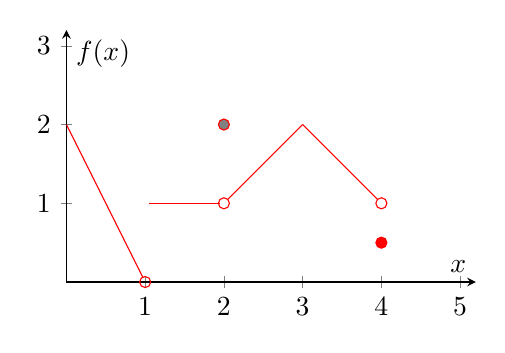
\begin{tikzpicture}
\begin{axis}[ axis x line=middle, axis y line=middle,xmax=5.2,ymax=3.2,xmin=0,ymin=0,ylabel=$f(x)$, xlabel=$x$, legend pos = north west,x=1cm,y=1cm]
\addplot[domain= 0:0.97, color = red]{-2*x+2};
\addplot[domain= 1.05:1.95, color = red]{1};
\addplot[domain= 2.05:3, color = red]{x-1};
\addplot[domain= 3:3.95, color = red]{-x+5};
\addplot+[only marks, mark = o,color = red] coordinates
{(1,0)};
\addplot+[only marks, mark = o,color = red] coordinates
{(2,1)};
\addplot+[only marks, mark = o,color = red] coordinates
{(4,1)};
\addplot+[only marks, mark = *,color = red] coordinates
{(2,2)};
\addplot+[only marks, mark = *,color = red] coordinates
{(4,0.5)};
    \end{axis}
\end{tikzpicture}
\end{center}

The function is \underline{\hbox to 5mm{}} (continuous/not continuous) on (0, 1)

The function is \underline{\hbox to 5mm{}} (continuous/not continuous) on (1, 3)

The function is \underline{\hbox to 5mm{}} (continuous/not continuous) on (2, 4)

\paragraph{发现}
上面的定义方式,好处是直观、快捷,坏处是非常不严谨。一个数学概念肯定不能是用“一笔能不能画出来”来定义的,下面我们就来观察一下continuous的几个必要因素。

\begin{center}
\begin{tikzpicture}
\begin{axis}[ axis x line=middle, axis y line=middle,xmax=5.2,ymax=3.2,xmin=0,ymin=0,ylabel=$f(x)$, xlabel=$x$, legend pos = north west,x=1cm,y=1cm]
\addplot[domain= 0:2, color = red]{2};
\addplot[domain= 3:5, color = red]{2};
    \end{axis}
\end{tikzpicture}
\end{center}

The function is \underline{\hbox to 5mm{}} (continuous/not continuous) on (2, 3)

函数图像“连续”起来,最最基本的条件是函数在某个区间得有“图像”吧?如果连图像都没有,就不用提连续不连续了。而有图像的前提条件是,函数在该点有定义。

所以第一个结论:

若函数$f(x)$在$x=a$处是continuous的,必要条件之一是$f(a)$\underline{\hbox to 5mm{}}(exist/not exist)

\begin{center}
\begin{tikzpicture}
\begin{axis}[ axis x line=middle, axis y line=middle,xmax=5.2,ymax=5.2,xmin=0,ymin=0,ylabel=$f(x)$, xlabel=$x$, legend pos = north west,x=1cm,y=1cm]
\addplot[domain= 0:2, color = red]{x^2};
\addplot[domain= 2:5, color = red]{-x/2+4};
\addplot +[style = loosely dashed, mark = none] coordinates {(2,-1) (2,5)};
    \end{axis}
\end{tikzpicture}
\end{center}

The function is \underline{\hbox to 5mm{}} (continuous/not continuous) on (1, 3)。

这一次,函数discontinuous的主要原因是在$x = 2$这一点出了篓子,也就是说,在$x = 2$这一点必须抬笔。我们管这种情况叫做“$f(x)$ is discontinuous at $x = 2$”。

出现了这样的问题,说白了就是如果从左往右看,$f(x)$“本该”等于4,却硬生生的“跳到”了3;如果从右往左看,那就是$f(x)$“本该”等于3,却硬生生的“跳到”了4。可惜、可惜。

那么如何用数学来表示“本该”呢?

从左往右看的话,“本该”是4,翻译成数学也就是说:

\[{\lim_{x \to 2^{\underline{\hbox to 5mm{}}}} f(x)} = \underline{\hbox to 5mm{}}\]

从右往左看的话,“本该”是3,翻译成数学也就是说:

\[{\lim_{x \to 2^{\underline{\hbox to 5mm{}}}} f(x)} = \underline{\hbox to 5mm{}}\]

所以就出现了这样的情况:

\[{\lim_{x \to 2^+} f(x)} \underline{\hbox to 5mm{}} {\lim_{x \to 2^-} f(x)} \]

从图像上看,也就是函数“断了”!

于是我们得到了第二个结论:

若函数$f(x)$在$x=a$处是continuous的,必要条件之二是\[{\lim_{x \to \underline{\hbox to 5mm{}}^{\underline{\hbox to 5mm{}}}} f(x)}   \underline{\hbox to 5mm{}}    {\lim_{x \to \underline{\hbox to 5mm{}}^{\underline{\hbox to 5mm{}}}} f(x)}\]

然而,只满足这两个条件是不够的,因为我们还会遇到这样的奇葩函数:

\begin{center}
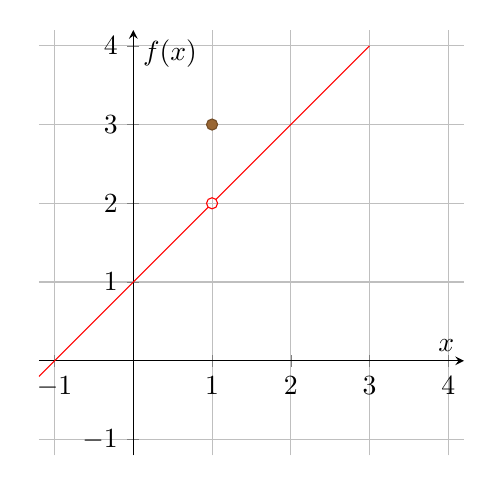
\begin{tikzpicture}
\begin{axis}[ axis x line=middle, axis y line=middle,xmax=4.2,ymax=4.2,xmin=-1.2,ymin=-1.2,ylabel=$f(x)$, xlabel=$x$, legend pos = north west,x=1cm,y=1cm,grid = major]
\addplot[domain= -1.2:0.95, color = red]{(x^2-1)/(x-1)};
\addplot+[only marks, mark = o] coordinates
{(1,2)};
\addplot+[only marks, mark = *] coordinates
{(1,3)};
\addplot[domain= 1.05:3, color = red]{(x^2-1)/(x-1)};
    \end{axis}
\end{tikzpicture}
\end{center}

我们来检视一下第一个条件是否符合?$f(x)$是在(-1,3)上面所有的点都有定义吗?\underline{\hbox to 5mm{}}(T/F)

我们来检视一下第一个条件是否符合?$f(x)$在其他点上显然是符合的,唯一比较特殊的点就是$x=1$这一个点。

从左边往右看,$f(x)$在$x=1$时的值“本该”是\underline{\hbox to 5mm{}}
\[{\lim_{x \to 1-} f(x)} = \underline{\hbox to 5mm{}}\]

从右边往左看,$f(x)$在$x=1$时的值“本该”是\underline{\hbox to 5mm{}}
\[{\lim_{x \to 1+} f(x)} = \underline{\hbox to 5mm{}}\]

\[{\lim_{x \to 1^+} f(x)} \underline{\hbox to 5mm{}} {\lim_{x \to 1^-} f(x)} \]

第二个条件是\underline{\hbox to 5mm{}}(符合/不符合)的。

那么问题出在哪呢?我们来观察$x=1$点和$x = 2$点。

在$x = 1$点处,$f(1) = \underline{\hbox to 5mm{}}$,同时${\lim_{x \to 1^+} f(x)} = {\lim_{x \to 1^-} f(x)} = \underline{\hbox to 5mm{}}$

在$x = 2$点处,$f(2) = \underline{\hbox to 5mm{}}$,同时${\lim_{x \to 2^+} f(x)} = {\lim_{x \to 2^-} f(x)} = \underline{\hbox to 5mm{}}$

在$x = 1$点处(discontinuous点),$f(1) \underline{\hbox to 5mm{}} {\lim_{x \to 1} f(x)}$

在$x = 2$点处(continuous点),$f(2) \underline{\hbox to 5mm{}} {\lim_{x \to 2} f(x)}$

这就是函数在$x=1$点处discontinuous的原因,于是我们总结出:

若函数$f(x)$在$x=a$处是continuous的,必要条件之三是$f(a) \underline{\hbox to 5mm{}} {\lim_{x \to a} f(x)}$。

\paragraph{总结}
对于函数$f(x)$,如果满足如下三个条件,我们就说$f(x)$在$x=a$这一点是continuous的:

1. $f(x)$ is defined at $x = a$。(确保函数在a点有图像)

2. ${\lim_{x \to a^-} f(x)} = {\lim_{x \to a^+} f(x)}$ (确保不出现“断崖”)

3. $f(a) = {\lim_{x \to a} f(x)}$ (确保不出现“空洞”)

\subsubsection{Types of Discontinuity}
[EK 1.2A3]

\paragraph{发现}
根据在图像上不同的表现方式,我们一般来说可以把Discontinuity分成三种不同的情况:

情况一:\textcolor{red}{Removable Discontinuity}(坑)
\begin{center}
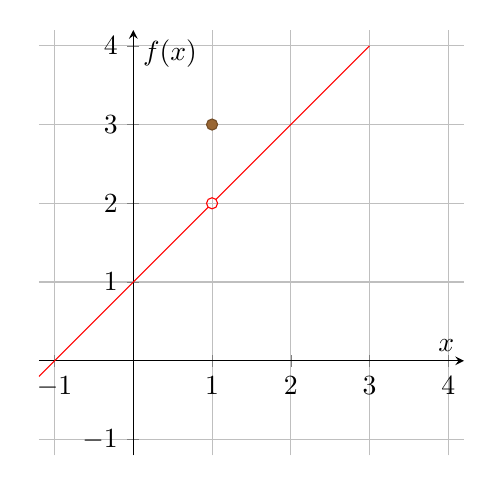
\begin{tikzpicture}
\begin{axis}[ axis x line=middle, axis y line=middle,xmax=4.2,ymax=4.2,xmin=-1.2,ymin=-1.2,ylabel=$f(x)$, xlabel=$x$, legend pos = north west,x=1cm,y=1cm,grid = major]
\addplot[domain= -1.2:0.95, color = red]{(x^2-1)/(x-1)};
\addplot+[only marks, mark = o] coordinates
{(1,2)};
\addplot+[only marks, mark = *] coordinates
{(1,3)};
\addplot[domain= 1.05:3, color = red]{(x^2-1)/(x-1)};
    \end{axis}
\end{tikzpicture}
\end{center}

说白了就是,沿着函数图像走,本来走着走着好好的,结果走到某点掉坑里了。但是只要修路工人过来修补一下,是可以把“坑”填上的。也就是说,这种discontinuity还不是特严重和离谱,是“removable”的。

造成这种discontinuity的原因应该是?\underline{\hbox to 5mm{}}
A. 未满足 $f(x)$ is defined at $x = a$。

B. 未满足${\lim_{x \to a^-} f(x)} = {\lim_{x \to a^+} f(x)}$

C. 未满足$f(a) = {\lim_{x \to a} f(x)}$ 

情况二:\textcolor{red}{Jump Discontinuity} (断崖)
\begin{center}
\begin{tikzpicture}
\begin{axis}[ axis x line=middle, axis y line=middle,xmax=5.2,ymax=5.2,xmin=0,ymin=0,ylabel=$f(x)$, xlabel=$x$, legend pos = north west,x=1cm,y=1cm]
\addplot[domain= 0:2, color = red]{x^2};
\addplot[domain= 2:5, color = red]{-x/2+4};
\addplot +[style = loosely dashed, mark = none] coordinates {(2,-1) (2,5)};
    \end{axis}
\end{tikzpicture}
\end{center}

也是走着走着掉下去了,但是比Removable Discontinuity更严重一点,这次是一个悬崖,靠修路工人是没法填补好了,不过如果你体育好的话可以“跳”下去或者“跳”上去(摔死不管),所以我们管他叫Jump Discontinuity。

造成这种discontinuity的原因应该是?\underline{\hbox to 5mm{}}
A. 未满足 $f(x)$ is defined at $x = a$。

B. 未满足${\lim_{x \to a^-} f(x)} = {\lim_{x \to a^+} f(x)}$

C. 未满足$f(a) = {\lim_{x \to a} f(x)}$ 

情况三:\textcolor{red}{Discontinuous due to Vertical Asymptotes}(由于该地有竖直渐近线造成的不连续)

比较经典的情况是:
\begin{center}
\begin{tikzpicture}
\begin{axis}[ axis x line=middle, axis y line=middle,xmax=5.2,ymax=5.2,xmin=-5.2,ymin=-5.2,ylabel=$f(x)$, xlabel=$x$, legend pos = north west,x=1cm,y=1cm]
\addplot[domain= -6:-0.1, color = red]{1/x};
\addplot[domain= 0.1:6, color = red]{1/x};
    \end{axis}
\end{tikzpicture}
\end{center}

根据我们学过的Vertical Asympototes【链接】的定义,某点的函数值要么是$\infty$,要么是$-\infty$的时候,函数在该点就不是Discontinuous了。这个比上一种还要更严重,你连跳都跳不了了,因为“无底深渊也在回望着你”。

造成这种discontinuity的原因应该是?\underline{\hbox to 5mm{}}
A. 未满足 $f(x)$ is defined at $x = a$。

B. 未满足${\lim_{x \to a^-} f(x)} = {\lim_{x \to a^+} f(x)}$

C. 未满足$f(a) = {\lim_{x \to a} f(x)}$ 

\paragraph{游戏}
判断以下函数在对应点的Discontinuity是哪一种:

A. Removable Discontinuity

B. Jump Discontinuity

C. Discontinuity due to Vertical Asymptotes

D. It's continuous.


\begin{center}
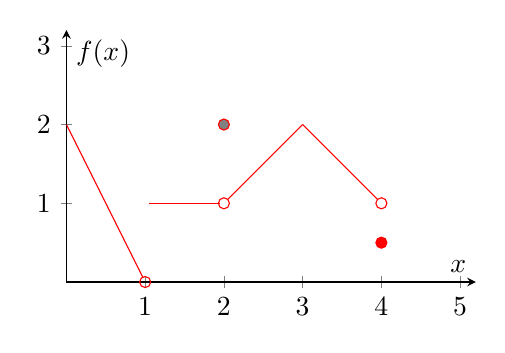
\begin{tikzpicture}
\begin{axis}[ axis x line=middle, axis y line=middle,xmax=5.2,ymax=3.2,xmin=0,ymin=0,ylabel=$f(x)$, xlabel=$x$, legend pos = north west,x=1cm,y=1cm]
\addplot[domain= 0:0.97, color = red]{-2*x+2};
\addplot[domain= 1.05:1.95, color = red]{1};
\addplot[domain= 2.05:3, color = red]{x-1};
\addplot[domain= 3:3.95, color = red]{-x+5};
\addplot+[only marks, mark = o,color = red] coordinates
{(1,0)};
\addplot+[only marks, mark = o,color = red] coordinates
{(2,1)};
\addplot+[only marks, mark = o,color = red] coordinates
{(4,1)};
\addplot+[only marks, mark = *,color = red] coordinates
{(2,2)};
\addplot+[only marks, mark = *,color = red] coordinates
{(4,0.5)};
    \end{axis}
\end{tikzpicture}
\end{center}

\[x = 1 \qquad \underline{\hbox to 5mm{}}\]
\[x = 2 \qquad \underline{\hbox to 5mm{}}\]
\[x = 3 \qquad \underline{\hbox to 5mm{}}\]
\[x = 4 \qquad \underline{\hbox to 5mm{}}\]

\begin{center}
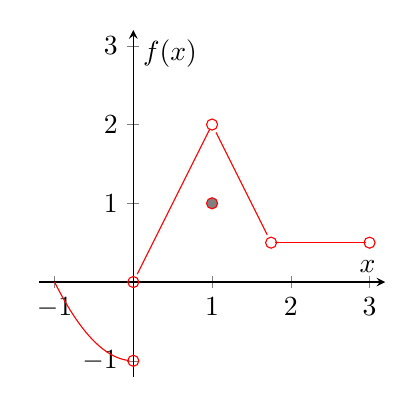
\begin{tikzpicture}
\begin{axis}[ axis x line=middle, axis y line=middle,xmax=3.2,ymax=3.2,xmin=-1.2,ymin=-1.2,ylabel=$f(x)$, xlabel=$x$, legend pos = north west,x=1cm,y=1cm]
\addplot[domain= -1:-0.05, color = red]{x^2-1};
\addplot[domain= 0.05:0.97, color = red]{2*x};
\addplot[domain= 1.05:1.70, color = red]{-2*x+4};
\addplot[domain= 1.80:2.95, color = red]{0.5};
\addplot+[only marks, mark = o,color = red] coordinates
{(0,-1)};
\addplot+[only marks, mark = o,color = red] coordinates
{(0,0)};
\addplot+[only marks, mark = o,color = red] coordinates
{(1,2)};
\addplot+[only marks, mark = *,color = red] coordinates
{(1,1)};
\addplot+[only marks, mark =o,color = red] coordinates
{(1.75,0.5)};
\addplot+[only marks, mark =o,color = red] coordinates
{(3,0.5)};
    \end{axis}
\end{tikzpicture}
\end{center}

\[x = -1 \qquad \underline{\hbox to 5mm{}}\]
\[x = 0 \qquad \underline{\hbox to 5mm{}}\]
\[x = 1 \qquad \underline{\hbox to 5mm{}}\]
\[x = 1.75 \qquad \underline{\hbox to 5mm{}}\]
\[x = 3 \qquad \underline{\hbox to 5mm{}}\]

\subsubsection{Continuous Functions}
[EK 1.2A2]
\paragraph{探索}
如果一个函数在一段区间上完全没有discontinuity(或者说continuous at every point),那么我们说这个函数\textcolor{red}{continuous on the interval}(在该区间上连续)。

如果一个函数continuous on its domain(在整个定义域都是连续的),我们就授予该函数荣誉称号\textcolor{red}{Continuous Function}(连续函数)以表彰该函数在道路建设上展现的突出成绩。

请注意以下这个函数:
\[f(x) = \frac{1}{x}\]
其domain为:
\[(-\infty, \underline{\hbox to 5mm{}}) \cup (\underline{\hbox to 5mm{}},\infty)\]
在该domain上,函数\underline{\hbox to 5mm{}}(有/无)discontinuous的点,所以该函数\underline{\hbox to 5mm{}}(是/非)continuous function;同时,该函数在$(-1,1)$区间内是\underline{\hbox to 5mm{}}(continuous/discontinuous)的。这说明,一个函数是continuous function,\underline{\hbox to 5mm{}}(一定/不一定)说明该函数在$(-\infty, \infty)$上是连续的。

\paragraph{游戏}
请说明如下函数:

1. 在哪一点是discontinuous的(若没有,填写N;如果在整个区间都discontinuous,则任意选该区间内的一个点)

2. 该点的discontinuous的类型(A. Removable  B.Jump C. Infinite )

3. 该函数是否是continuous function.

(主线任务)
\[f(x) = \frac{x^2-x-2}{x+1}\]
$f(x)$在$x = \underline{\hbox to 5mm{}}$处是discontinuous的

该discontinuous的类型是\underline{\hbox to 5mm{}}。

该函数\underline{\hbox to 5mm{}}(是/不是)continuous function

\[f(x) = 
\begin{cases}
\frac{x^2-x-2}{x+1} & x \neq -1\\
0 & x=-1
\end{cases}
\]
$f(x)$在$x = \underline{\hbox to 5mm{}}$处是discontinuous的

该discontinuous的类型是\underline{\hbox to 5mm{}}。

该函数\underline{\hbox to 5mm{}}(是/不是)continuous function

\[f(x) = 
\begin{cases}
x^2-3x+9 & x < 2\\
3x+1 & x > 3
\end{cases}
\]
$f(x)$在$x = \underline{\hbox to 5mm{}}$处是discontinuous的

该discontinuous的类型是\underline{\hbox to 5mm{}}。

该函数\underline{\hbox to 5mm{}}(是/不是)continuous function

\[f(x) = 
\begin{cases}
x^2-3x+9 & x < 2\\
3x+1 & x > 2
\end{cases}
\]
$f(x)$在$x = \underline{\hbox to 5mm{}}$处是discontinuous的

该discontinuous的类型是\underline{\hbox to 5mm{}}。

该函数\underline{\hbox to 5mm{}}(是/不是)continuous function

\[f(x) = 
\begin{cases}
x^2-3x+9 & x \leq 2\\
3x+1 & x > 2
\end{cases}
\]
$f(x)$在$x = \underline{\hbox to 5mm{}}$处是discontinuous的

该discontinuous的类型是\underline{\hbox to 5mm{}}。

该函数\underline{\hbox to 5mm{}}(是/不是)continuous function

\paragraph{发现}
我们知道一些非常基本的函数很明显是continuous function,例如$f(x) = x$、$f(x) = x^2$这些。那么如何判断一些比较复杂的函数是否是continuous function呢?难道每一个都要画出来?或者每一函数我们都需要对它domain内的每一个点进行检查,看看那个点是否是“断的”?这样工作量太大了,数学的魅力在于“偷懒”。我们需要总结一个规律,以快速判断某个函数是否是continuous function。

我们假设$f(x)$在$x = a$点连续,$g(x)$也在$x = a$点连续。那么$f(x) + g(x)$是不是在$x = a$点也连续呢?

1. $f(x)$ is continuous at $x = a$
\[ \Longrightarrow f(x) \text{ is } \underline{\hbox to 5mm{}} \text{ (defined/not defined) at } x = a \] 
$g(x)$ is continuous at $x = a$
\[ \Longrightarrow g(x) \text{ is } \underline{\hbox to 5mm{}} \text{ (defined/not defined) at } x = a \] 
 $f(x)$ and $g(x)$ is both \underline{\hbox to 5mm{}}(defined/not defined) at $x = a$
 \[\Longrightarrow f(x)+g(x) \text{is} \underline{\hbox to 5mm{}}\text{(defined/not defined) at }x = a\](连续性的第一项条件:有定义,满足!)

2. $f(x)$ is continuous at $x = a$
\[ \Longrightarrow {\lim_{x \to a-}f(x) =} \underline{\hbox to 5mm{}} ( = / \neq)  {\lim_{x \to a+}f(x)} \] 
$g(x)$ is continuous at $x = a$
\[ \Longrightarrow {\lim_{x \to a-}g(x) =} \underline{\hbox to 5mm{}} ( = / \neq)  {\lim_{x \to a+}g(x)} \] 
 \[\Longrightarrow {\lim_{x \to a-}f(x)} +  {\lim_{x \to a-}g(x)} \underline{\hbox to 5mm{}} ( = / \neq)  {\lim_{x \to a+}f(x)} + {\lim_{x \to a+}g(x)}\]
Apply limit theorem:
\[{\lim_{x \to a} f(x) + g(x)} = {\lim_{x \to a} f(x)}  + {\lim_{x \to a} g(x)} \text{【链接】}\]
  \[\Longrightarrow {\lim_{x \to a-}[f(x) + g(x)]}\underline{\hbox to 5mm{}} ( = / \neq)  {\lim_{x \to a+}[f(x) + g(x)]}\]
 (连续性的第二项条件:无断崖,满足!)

3. $f(x)$ is continuous at $x = a$
\[ \Longrightarrow {\lim_{x \to a}f(x)} = f(a) \] 
$g(x)$ is continuous at $x = a$
\[ \Longrightarrow {\lim_{x \to a}g(x)} = g(a) \] 
\[ \Longrightarrow {\lim_{x \to a}f(x)} + {\lim_{x \to a}g(x)} = \underline{\hbox to 5mm{}} \] 
Apply limit theorem:
\[{\lim_{x \to a} f(x) + g(x)} = {\lim_{x \to a} f(x)}  + {\lim_{x \to a} g(x)} \text{【链接】}\]
\[ \Longrightarrow {\lim_{x \to a}f(x)+g(x)} = \underline{\hbox to 5mm{}} \] 
(连续性的第三项条件:无断点,满足!)

三项连续性条件均满足,说明$f(x) + g(x)$在$x = a$处\underline{\hbox to 5mm{}}(continuous/discontinuous)!

所以我们知道:

若$f(x)$、$g(x)$在$x = a$处是continuous的,那么$f(x)+g(x)$在$x=a$是\underline{\hbox to 5mm{}}(continuous/discontinuous)的。

若$f(x)$、$g(x)$是continuous function,那么$f(x) + g(x)$ 是\underline{\hbox to 5mm{}}(continuous/discontinuous)function。

\paragraph{总结}
以上推导过程适用于全部的五个Limit Theorem,故我们可以得到结论:

If the functions $f(x)$ and $g(x)$ are continuous at $x = a$, then the following combinations are continuous at $x = a$:

1. Sums: $f(x) + g(x)$

2. Differences: $f(x) - g(x)$

3. Products: $f(x) \cdot g(x)$

4. Quotients: $\frac{f(x)}{g(x)}$, if $g(x) \neq 0$

5. Powers: $f(x)^{r/s}$, if r and s are integers

\paragraph{发现}
我们学过的基本初等函数,全部都是continuous function,包括:

Power Functions: $f(x) = x^a$, for any real number a.

Exponential Functions: $f(x) = a^x$, provided $a>0$.

Logarithmic Functions: $f(x) = log_a x$, provided $a>0$.

Trigonometric Functions: $f(x) = \sin{x}$ 、$f(x) = \cos{x}$、$f(x) = \tan{x}$、$f(x) = \cot{x}$、$f(x) = \sec{x}$、$f(x) = \csc{x}$

如果我们再使用刚才的五个规则,我们就可以制造出无数“continuous function”,只要他们是这些基本初等函数的组合。

另外,很明显:以下两种函数其实就是Power Functions的组合,也一定是连续的:

Limits of Polynomials(多项式函数)
\[f(x) = a_nx^n + a_{n-1}x^{n-1}+\cdots+a_0\]

Limits of Rational Functions as long as the denominator is non-zero(有理函数,只要分母不为0)
\[\text{If } f(x) \text{ and } g(x) \text{ are polynomials, then $\frac{f(x)}{g(x)}$ is continuous function}\]

\paragraph{发现}
除了加、减、乘、除、乘方以外,在组合两个函数时,还有一种比较特殊的组合方法:Composite(复合)
\[f(x) \circ g(x) = f[g(x)]\]
我们关注的是,如果对复合之后的函数求极限,会得到什么结果?我们可以大胆“猜测”一下:
\[{\lim_{x \to a}f[g(x)] }= f[{\lim_{x \to a} \underline{\hbox to 5mm{}}}] \]
这个猜测是正确的,证明我们就不在这里讨论了。该定理成立的前提是:

1. ${\lim_{x \to a} g(x)}$ 存在。(这是必须的,不存在的话怎么扔进$f(x)$里面去)

2. $f(x)$在${\lim_{x \to a} g(x)}$点处是continuous的。

\[{\lim_{x \to 1} \arcsin{\frac{\sqrt{x} - 1}{ x - 1}}}\]
检查:1. ${\lim_{x \to 1} \frac{\sqrt{x} - 1}{ x - 1}}$是否存在?
\begin{eqnarray*}
{\lim_{x \to 1} \frac{\sqrt{x} - 1}{ x - 1}} & = & {\lim_{x \to 1} \frac{\sqrt{x} - 1}{ x - 1} \cdot \frac{\underline{\hbox to 5mm{}} + \underline{\hbox to 5mm{}}}{\underline{\hbox to 5mm{}} + \underline{\hbox to 5mm{}}}}  \\
& = & {\lim_{x \to 1} \frac{\underline{\hbox to 5mm{}}-\underline{\hbox to 5mm{}}}{(x-1) \cdot (\underline{\hbox to 5mm{}}+\underline{\hbox to 5mm{}}) }} \\
& = & {\lim_{x \to 1} \frac{1}{\underline{\hbox to 5mm{}}+\underline{\hbox to 5mm{}}}}\\
& = & \underline{\hbox to 5mm{}}
\end{eqnarray*} 
存在!

检查:2. $f(x) = \arcsin{x}$在$x = 1$点处是continuous的吗?
$\arcsin{x}$是trigonometric function,所以它在$x = \frac{1}{2}$\underline{\hbox to 5mm{}}(是/不是)continuous的。

所以:\[{\lim_{x \to 1} \arcsin{\frac{\sqrt{x} - 1}{ x - 1}}} = \arcsin{{\lim_{x \to 1} \frac{\sqrt{x} - 1}{ x - 1}}} = \arcsin{\frac{1}{2}} =\underline{\hbox to 5mm{}}\]

\paragraph{游戏}
求以下composite function(复合函数)的limit:
\begin{center}
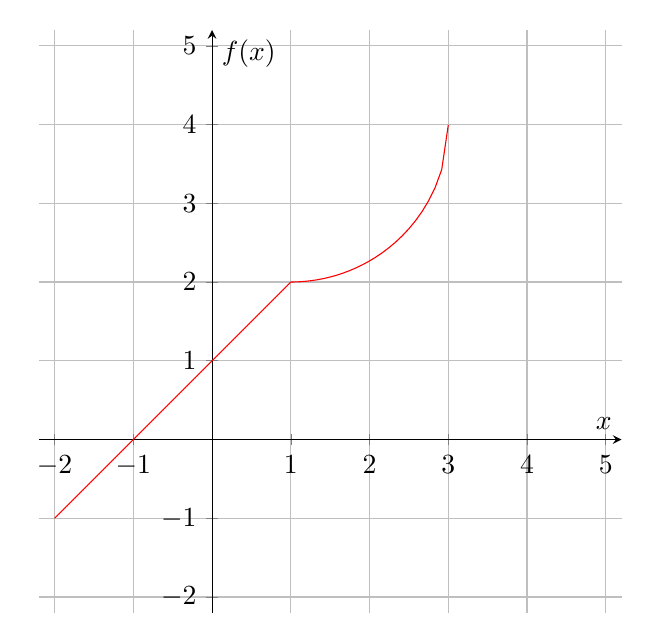
\begin{tikzpicture}
\begin{axis}[ axis x line=middle, axis y line=middle,xmax=5.2,ymax=5.2,xmin=-2.2,ymin=-2.2,ylabel=$f(x)$, xlabel=$x$, legend pos = north west,x=1cm,y=1cm,grid = major]
\addplot[domain= -2:1, color = red]{x+1};
\addplot[domain= 1:3, color = red]{-(4-(x-1)^2)^0.5+4};
    \end{axis}
\end{tikzpicture}
\[f(x)\]
\end{center}

\begin{center}
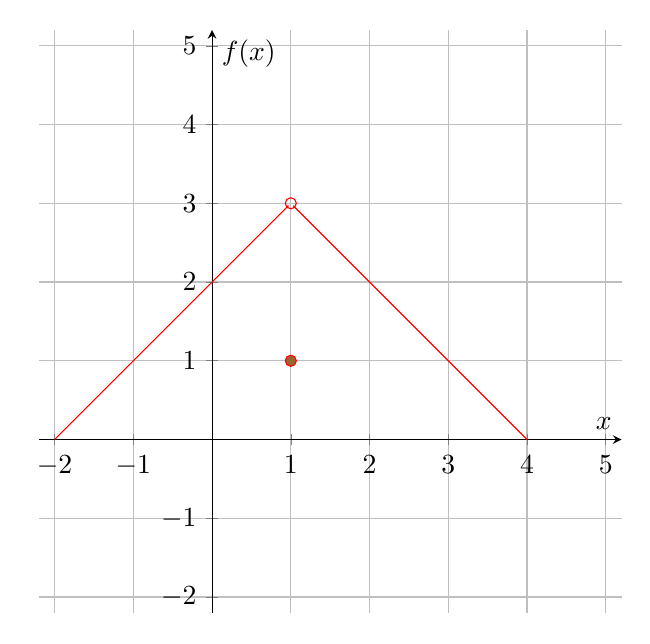
\begin{tikzpicture}
\begin{axis}[ axis x line=middle, axis y line=middle,xmax=5.2,ymax=5.2,xmin=-2.2,ymin=-2.2,ylabel=$f(x)$, xlabel=$x$, legend pos = north west,x=1cm,y=1cm,grid = major]
\addplot[domain= -2:0.97, color = red]{x+2};
\addplot+[only marks, mark = o,color = red] coordinates
{(1,3)};
\addplot+[only marks, mark = *,color = red] coordinates
{(1,1)};
\addplot[domain= 1.03:4, color = red]{-x+4};
    \end{axis}
\end{tikzpicture}
\[g(x)\]
\end{center}

\[{\lim_{x \to 1} f[g(x)]} = ?\]
\[{\lim_{x \to 1} g(x) = \underline{\hbox to 5mm{}}}\]
\[{\lim_{x \to 1} f[g(x)]} = f[{\lim_{x \to 1} g(x)}] = \underline{\hbox to 5mm{}}\]

\paragraph{发现}
因为和加、减、乘、除和乘方同样的原因,我们了解了复合函数的limit原则以后,就可以推断出复合函数的continuity原则:
\[\text{如果} g(x)\text{在}x = c\text{处是continuous的,同时}f\text{在}g(c)\text{处是continuous的,那么}f[g(x)]\text{在}x = c\text{处也是continuous的。}\]

\[F(x) = \sqrt{x^2-2x-4}\]
该函数分为两层,外层函数为$f(x) = $\underline{\hbox to 5mm{}};内层函数为$g(x) = $\underline{\hbox to 5mm{}}。$g(x)$在$x \in \underline{\hbox to 5mm{}},\underline{\hbox to 5mm{}}$的区间上continuous; $f(x)$在$x \in \underline{\hbox to 5mm{}},\underline{\hbox to 5mm{}}$的区间上continuous;所以函数$F(x)$在$x \in \underline{\hbox to 5mm{}},\underline{\hbox to 5mm{}}$的区间上continuous。

 \[F(x) = \sin{(\sin{x} -x)}\]
该函数分为两层,外层函数为$f(x) = $\underline{\hbox to 5mm{}};内层函数为$g(x) = $\underline{\hbox to 5mm{}}。$g(x)$在$x \in \underline{\hbox to 5mm{}},\underline{\hbox to 5mm{}}$的区间上continuous; $f(x)$在$x \in \underline{\hbox to 5mm{}},\underline{\hbox to 5mm{}}$的区间上continuous;所以函数$F(x)$在$x \in \underline{\hbox to 5mm{}},\underline{\hbox to 5mm{}}$的区间上continuous。

\[F(x) = \sin{(\frac{\pi}{2} \cdot \cos{(\cot{x})})}\]
该函数分为两层,外层函数为$f(x) = $\underline{\hbox to 5mm{}};内层函数为$g(x) = $\underline{\hbox to 5mm{}}。$g(x)$在$x \in \underline{\hbox to 5mm{}},\underline{\hbox to 5mm{}}$的区间上continuous; $f(x)$在$x \in \underline{\hbox to 5mm{}},\underline{\hbox to 5mm{}}$的区间上continuous;所以函数$F(x)$在$x \in \underline{\hbox to 5mm{}},\underline{\hbox to 5mm{}}$的区间上continuous。

\paragraph{游戏}
判断以下函数在哪个区间不continuous。如果函数在某一点不continuous,则也可以用区间表示,如$x=3$处不continuous可以写做$x \in [3,3]$区间内不continuous。
(主线任务)
\[f(x) = \frac{1}{x-1} - 3x \qquad f(x) = \frac{1}{(x+1)^2} +4\]
\[f(x) = \frac{x+1}{x^2-5x+6} \qquad f(x) = \frac{x+3}{x^2 -3x - 18}\]
\[f(x) = |x+1|+\cos{x} \qquad f(x) = \frac{1}{|x|-1} -\frac{x^2}{2}\]
 \[f(x) = \sqrt[4]{2x-1} \qquad f(x) = (2-x)^{\frac{1}{5}}\] 
 \[f(x) = \cos{(\frac{\pi}{\sqrt{19-4\sec2x}})} \qquad f(x) = \sqrt{\csc^2{x} +3\sqrt{3}\tan{x}}\] 
 

\subsubsection{The Intermediate Value Theorem}
[EK 1.2B1]
\paragraph{探索}
continuous function有许多非常重要的特性。比如我们之前曾经提到过的,每天的时间和温度之间的变化关系。
\begin{center}
\includegraphics[height = 3cm] {wendu}
\end {center}
我们知道,温度从早上8点的15度逐渐上升至中午12点的20度,是一个连续变化的过程,也就是说温度相对于时间的函数是continuous function。这暗示了从早上8点到中午12点之间,\underline{\hbox to 5mm{}}(必然/不一定)有一个瞬间,此时温度刚好等于18.4545353453224度。

也就是说,对于任意一个15~20之间的温度$f(t)$,一定有一个瞬间$t = T$,这个时候$f(t)$刚刚好等于这个温度。

我们将这个对于“连续”的感性理解推而广之到用数学的方式表达,就是:

如果函数$f(x)$在区间$[a,b]$上连续,那么\textcolor{red}{一定}存在某个值$a < x_0 < b$,使得$f(x_0)$可以等于任何介于$f(a)$与$f(b)$中间的值。

\begin{center}
     \begin{tikzpicture}

        \begin{axis}[
            xmin=-0.1,xmax=5,
            xlabel={z},
            ymin=0,ymax=4.5,
        xtick={1.27, 3, 4},
        xticklabels={$a$,$x_0$,$b$},
        ytick={1.5,2.32,3.5},
        yticklabels={$f(a)$,$f(x_0)$,$f(b)$},
        xlabel={$x$},  
        ylabel={$y$},
        axis lines=middle] 
    \draw [color=black,fill=white,thick,dashed] (axis cs:0,0) rectangle (axis cs:4,3.5);
    \draw [color=black,fill=white,thick,dashed] (axis cs:0,0) rectangle (axis cs:3,2.32);
    \draw [color=black,fill=white,thick,dashed] (axis cs:0,0) rectangle (axis cs:1.27,1.5);
    \draw [fill=black] (axis cs:0,0) rectangle (axis cs:0.01,4.45);
    \addplot+[black,thick,domain=0:5,no marks] {0};
    %
    %
    \end{axis}
  %Hobby package  
    \draw [thick] (1 ,1) to [ curve through ={(1.5,1.5)  . . (3,3) . . (4.5,3)  }] (5.5,4.5);% curve 
    \end{tikzpicture}
\end{center}

相反,如果一个函数不连续,比如如下的情况:
\begin{center}
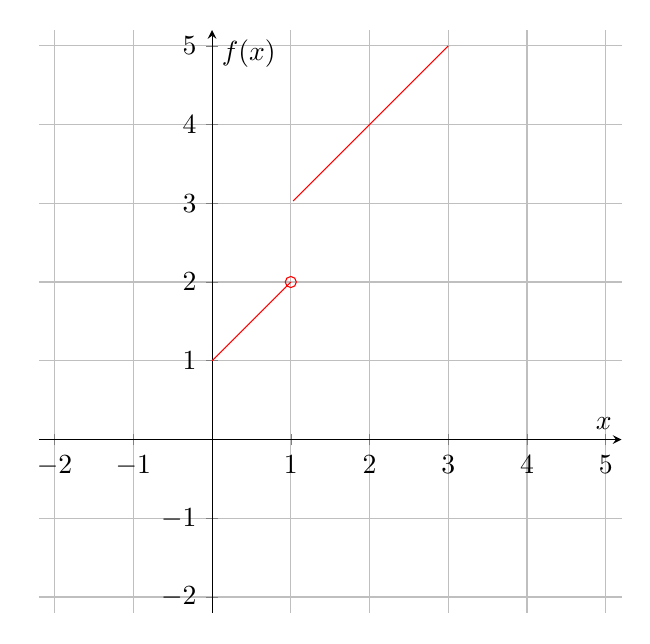
\begin{tikzpicture}
\begin{axis}[ axis x line=middle, axis y line=middle,xmax=5.2,ymax=5.2,xmin=-2.2,ymin=-2.2,ylabel=$f(x)$, xlabel=$x$, legend pos = north west,x=1cm,y=1cm,grid = major]
\addplot[domain= 0:1, color = red]{x+1};
\addplot[domain= 1.03:3, color = red]{x+2};
\addplot+[only marks, mark = o,color = red] coordinates
{(1,2)};
    \end{axis}
\end{tikzpicture}
\[f(x)\]
\end{center}
函数$f(x) = x$在$[0,3]$上\underline{\hbox to 5mm{}}(连续/不连续),$f(0) = $\underline{\hbox to 5mm{}}、$f(3) = $\underline{\hbox to 5mm{}}。我们在$f(0)$与$f(3)$之间选择一数$L = 2.5$,是否存在一个值$0<x_0<3$,使得$f(x_0) = 2.5$?\underline{\hbox to 5mm{}}。

函数$f(x) = x$在$[1,5]$上连续,$f(1) = $\underline{\hbox to 5mm{}}、$f(5) = $\underline{\hbox to 5mm{}},我们在$f(1)$与$f(5)$之间选择一数$L = 2.5$,是否存在一个值$1<x_0<5$,使得$f(x_0) = 2.5$?\underline{\hbox to 5mm{}}。


函数$f(x) = -x^2$在$[1,3]$上连续,$f(1) = $\underline{\hbox to 5mm{}}、$f(3) = $\underline{\hbox to 5mm{}},我们在$f(1)$与$f(3)$之间选择一数$L = 6$,是否存在一个值$1<x_0<3$,使得$f(x_0) = 6$?\underline{\hbox to 5mm{}}。


函数$f(x) = \sin{x}$在$[0, \pi]$上连续,$f(0) = $\underline{\hbox to 5mm{}}、$f(\pi) = $\underline{\hbox to 5mm{}},我们在$f(0)$与$f(\pi)$之间选择一数$L = \underline{\hbox to 5mm{}}$,是否存在一个值$0<x_0<\pi$,使得$f(x_0) = \underline{\hbox to 5mm{}}$?\underline{\hbox to 5mm{}}。

函数$f(x) = \frac{1}{x-2} -3x$在[3,5]上连续,$f(0) = $\underline{\hbox to 5mm{}}、$f(\pi) = $\underline{\hbox to 5mm{}},我们在$f(0)$与$f(\pi)$之间选择一数$\underline{\hbox to 5mm{}}<L< \underline{\hbox to 5mm{}}$,则必然存在一个值$\underline{\hbox to 5mm{}}<x_0< \underline{\hbox to 5mm{}}$, 使得$f(x_0) = L$。

函数$f(x) = \frac{1}{|x|+2} -\frac{x^2}{3}$在[-2,2]上连续,$f(-2) = $\underline{\hbox to 5mm{}}、$f(2) = $\underline{\hbox to 5mm{}},我们在$f(-2)$与$f(2)$之间选择一数$\underline{\hbox to 5mm{}}<L< \underline{\hbox to 5mm{}}$,则必然存在一个值$\underline{\hbox to 5mm{}}<x_0< \underline{\hbox to 5mm{}}$, 使得$f(x_0) = L$。

函数$f(x) = \frac{10^x-1}{x}$在(0,4)上连续,$f(0) = $\underline{\hbox to 5mm{}}、$f(\pi) = $\underline{\hbox to 5mm{}},我们在$f(0)$与$f(4)$之间选择一数$\underline{\hbox to 5mm{}}<L< \underline{\hbox to 5mm{}}$,则必然存在一个值$\underline{\hbox to 5mm{}}<x_0< \underline{\hbox to 5mm{}}$, 使得$f(x_0) = L$。

\paragraph{发现}
如果我们让$f(a)$和$f(b)$的符号一个为正,一个为负的话,那么根据Intermediate Value Theorem,必然存在一个值$x_0$,使得$f(x_0) = 0$。也就是说,函数$f(x)$\textcolor{red}{必有root(根)}。

我们尝试用这个方法,大概估算出
\[4x^3 - 6x^2 + 3x -2 =0\]
的一个root:
首先我们尝试$x = 0$与$x = 3$之间是否有root?设$f(x) = 4x^3 - 6x^2 + 3x -2 =0$,我们可以知道:
\[f(0) = \underline{\hbox to 5mm{}} \qquad f(0) \underline{\hbox to 5mm{}} (>/</=) 0\]
\[f(3) = \underline{\hbox to 5mm{}} \qquad f(3) \underline{\hbox to 5mm{}} (>/</=) 0\]
所以方程的root\underline{\hbox to 5mm{}}(在/不在)$[0,3]$之间。

接下来我们可以缩小范围,我们尝试一下$x = 1$与$x = 2$之间是否有root?
\[f(1) = \underline{\hbox to 5mm{}} \qquad f(0) \underline{\hbox to 5mm{}} (>/</=) 0\]
\[f(2) = \underline{\hbox to 5mm{}} \qquad f(3) \underline{\hbox to 5mm{}} (>/</=) 0\]
所以方程的root\underline{\hbox to 5mm{}}(在/不在)$[1,2]$之间。

继续缩小范围,可以尝试$x = 1.3$与$x = 1.6$之间是否有root(使用计算器,保留两位小数)?
\[f(1) = \underline{\hbox to 5mm{}} \qquad f(0) \underline{\hbox to 5mm{}} (>/</=) 0\]
\[f(2) = \underline{\hbox to 5mm{}} \qquad f(3) \underline{\hbox to 5mm{}} (>/</=) 0\]
所以方程的root\underline{\hbox to 5mm{}}(在/不在)$[1.3,1.6]$之间。

继续缩小范围,可以尝试$x = 1.2$与$x = 1.3$之间是否有root(使用计算器,保留两位小数)?
\[f(1.2) = \underline{\hbox to 5mm{}} \qquad f(0) \underline{\hbox to 5mm{}} (>/</=) 0\]
\[f(1.3) = \underline{\hbox to 5mm{}} \qquad f(3) \underline{\hbox to 5mm{}} (>/</=) 0\]
所以方程的root\underline{\hbox to 5mm{}}(在/不在)$[1.2,1.3]$之间。

\[\cos{x} = x^3\]是否存在root?首先,令$f(x) = \cos{x} - x^3$,寻找root的任务就变成了,寻找是否存在$x$,使得$f(x) = \underline{\hbox to 5mm{}}$。
根据Intermediate Value Theorem,如果存在$x_0$使得$f(x_0) = 0$,则必有$x_0 \in [a,b]$,且$f(a) \underline{\hbox to 5mm{}} 0、f(b) \underline{\hbox to 5mm{}} 0$或$f(a) \underline{\hbox to 5mm{}} 0、f(b)  \underline{\hbox to 5mm{}} 0$,也就是说$f(a)\cdot f(b)  \underline{\hbox to 5mm{}} 0$。
是否能找到这样的一对儿a,b,使得$f(a)\cdot f(b) < 0$ ? \underline{\hbox to 5mm{}}

\[\ln{x} = 3-2x\]是否存在root?首先,令$f(x) = \ln{x} - 3+2x$,寻找root的任务就变成了,寻找是否存在$x$,使得$f(x) = \underline{\hbox to 5mm{}}$。
根据Intermediate Value Theorem,如果存在$x_0$使得$f(x_0) = 0$,则必有$x_0 \in [a,b]$,且$f(a) \underline{\hbox to 5mm{}} 0、f(b) \underline{\hbox to 5mm{}} 0$或$f(a) \underline{\hbox to 5mm{}} 0、f(b)  \underline{\hbox to 5mm{}} 0$,也就是说$f(a)\cdot f(b)  \underline{\hbox to 5mm{}} 0$。
是否能找到这样的一对儿a,b,使得$f(a)\cdot f(b) < 0$ ? \underline{\hbox to 5mm{}}

\[x^2= -1-x\]是否存在root?首先,令$f(x) = x^2+x+1$,寻找root的任务就变成了,寻找是否存在$x$,使得$f(x) = \underline{\hbox to 5mm{}}$。
根据Intermediate Value Theorem,如果存在$x_0$使得$f(x_0) = 0$,则必有$x_0 \in [a,b]$,且$f(a) \underline{\hbox to 5mm{}} 0、f(b) \underline{\hbox to 5mm{}} 0$或$f(a) \underline{\hbox to 5mm{}} 0、f(b)  \underline{\hbox to 5mm{}} 0$,也就是说$f(a)\cdot f(b)  \underline{\hbox to 5mm{}} 0$。
是否能找到这样的一对儿a,b,使得$f(a)\cdot f(b) < 0$ ? \underline{\hbox to 5mm{}}


\end{document}